\documentclass[12pt,a4paper]{article}
\usepackage{graphicx}
\usepackage{geometry}
\usepackage{mathptmx} % Times New Roman
\usepackage{setspace}
\onehalfspacing
\usepackage{booktabs}
\usepackage{threeparttable} % Add to preamble
\usepackage{cite}
\usepackage{amsmath,amssymb}
\usepackage{hyperref}
\usepackage{multirow}
\usepackage{array}
\usepackage{xcolor}
\usepackage{colortbl}
\usepackage{longtable}
\usepackage{pdflscape}
\usepackage{caption}
\usepackage{subcaption}
\usepackage{float}
\usepackage{xurl}
\usepackage{enumitem}
% \usepackage{microtype}

% Start sections on new pages
\usepackage{titlesec}
\newcommand{\sectionbreak}{\clearpage}
% Format sections as chapters
\titleformat{\section}[display]
  {\normalfont\Large\bfseries\centering}
  {Chapter \thesection}
  {1ex}
  {\MakeUppercase}

% Number figures and tables by section
\usepackage{chngcntr}
\counterwithin{figure}{section}
\counterwithin{table}{section}

% Center Table of Contents, List of Figures, and List of Tables titles
\makeatletter
\renewcommand\tableofcontents{%
    \section*{\centering\contentsname}%
    \@starttoc{toc}%
}
\renewcommand\listoffigures{%
    \section*{\centering\listfigurename}%
    \@starttoc{lof}%
}
\renewcommand\listoftables{%
    \section*{\centering\listtablename}%
    \@starttoc{lot}%
}
\makeatother

\geometry{a4paper, left=1.5in, right=1in, top=1in, bottom=1in}
\captionsetup{font=small, labelfont=bf, skip=6pt}
\usepackage{iftex}
\ifXeTeX
  \usepackage{fontspec}
  \newfontfamily\banglafont[Script=Bengali]{Kalpurush}
\else
  \providecommand{\banglafont}{}
\fi
\ifdefined\DeclareUnicodeCharacter
  \DeclareUnicodeCharacter{0964}{\textbar}
\fi

\begin{document}

\begin{titlepage}
\centering
\vspace*{1cm}
{\Large \textbf{\MakeUppercase{Comparative Analysis of Locally Produced Bitumen and Imported Low-Cost Bitumen for Bangladesh Road Construction (Focusing on Aggregate Shape)}}}\par
\vspace{1cm}
A Thesis [CE 400]\\
\vspace{1cm}
by\\
\vspace{1cm}
Md Rakibul Hasan Mridha (2020333545)\\
Md Sagor Hossain Saddas (2020333553)\\
\vspace{1.5cm}
BACHELOR OF SCIENCE IN CIVIL ENGINEERING\\
\vspace{1.5cm}

\includegraphics[width=1.7in,height=1.7in]{graphics/sec logo.png}\\
\vspace{1.5cm}
DEPARTMENT OF CIVIL ENGINEERING\\
SYLHET ENGINEERING COLLEGE\\
SYLHET-3100, BANGLADESH\\
\vspace{1cm}
September, 2026
\end{titlepage}

\begin{titlepage}
\centering
\vspace*{1cm}
{\Large \textbf{\MakeUppercase{Comparative Analysis of Locally Produced Bitumen and Imported Low-Cost Bitumen for Bangladesh Road Construction (Focusing on Aggregate Shape)}}}\par
\vspace{1cm}
by\\
\vspace{1cm}
Md Rakibul Hasan Mridha (2020333545)\\
Md Sagor Hossain Saddas (2020333553)\\
\vspace{1.5cm}
A thesis submitted to the Department of Civil Engineering in partial fulfillment for the degree of\\
BACHELOR OF SCIENCE IN CIVIL ENGINEERING\\
\vspace{1cm}
At the\\
SYLHET ENGINEERING COLLEGE\\
Affiliated with Shahjalal University of Science and Technology (SUST), Sylhet\\
\vspace{1cm}

\includegraphics[width=1.7in,height=1.7in]{graphics/sec logo.png}\\
\vspace{1cm}
DEPARTMENT OF CIVIL ENGINEERING\\
SYLHET ENGINEERING COLLEGE\\
SYLHET-3100, BANGLADESH\\
\vspace{1cm}
September, 2026
\end{titlepage}

\newpage
\pagenumbering{roman}
\phantomsection
\addcontentsline{toc}{section}{Declaration}

\begin{center}
    \textbf{\Large DECLARATION}
\end{center}

\vspace{3\baselineskip}

\noindent I hereby declare that this thesis/project is the result of my own independent work, and to the best of my knowledge, it contains no material previously published or written by another person, nor has it been submitted for the award of any degree at Sylhet Engineering College (SEC) or any other academic institution, except where proper acknowledgment has been made. This thesis was carried out by us under the supervision of Md Johir Bin Alam and Mohiuddin Arif.

I further affirm that the intellectual content of this work is entirely my own. Any contributions to the research by collaborators at this college or elsewhere have been clearly acknowledged.

\vspace{2cm}

\noindent
\begin{minipage}[t]{0.45\textwidth}
    \rule{0.8\textwidth}{0.5pt}\\
    Signature\\[0.5cm]
    Md Rakibul Hasan Mridha\\
    Reg. No.: 2020333545
\end{minipage}
\hfill
\begin{minipage}[t]{0.45\textwidth}
    \rule{0.8\textwidth}{0.5pt}\\
    Signature\\[0.5cm]
    Md Sagor Hossain Saddas\\
    Reg. No.: 2020333553
\end{minipage}

\newpage
\phantomsection
\addcontentsline{toc}{section}{Certification}

\begin{center}
    \textbf{\Large CERTIFICATION}
\end{center}

\vspace{2\baselineskip}

\begin{center}
{\large \textbf{\MakeUppercase{Comparative Analysis of Locally Produced Bitumen and Imported Low-Cost Bitumen for Bangladesh Road Construction (Focusing on Aggregate Shape)}}}\par
\vspace{1cm}
by\\
\vspace{1cm}
Md Rakibul Hasan Mridha (2020333545)\\
Md Sagor Hossain Saddas (2020333553)\\
\vspace{1cm}
A thesis submitted to the Department of Civil Engineering in partial fulfillment for the degree of\\
BACHELOR OF SCIENCE IN CIVIL ENGINEERING\\
\vspace{0.5cm}
At the\\
SYLHET ENGINEERING COLLEGE\\
Affiliated with Shahjalal University of Science and Technology (SUST), Sylhet\\
\end{center}

\vspace{1.5cm}
\noindent APPROVED AS TO STYLE AND CONTENT BY:

\vspace{2.5cm}

\noindent
\begin{minipage}[t]{0.48\textwidth}
    \rule{2.5in}{0.5pt}\\
    Md Johir Bin Alam\\
    Professor, Department of CEE\\
    Shahjalal University of Science \& Technology\\
    Sylhet-3100
\end{minipage}
\hfill
\begin{minipage}[t]{0.48\textwidth}
    \rule{2.5in}{0.5pt}\\
    Mohiuddin Arif\\
    Lecturer, Department of Civil Engineering\\
    Sylhet Engineering College\\
    Sylhet-3100
\end{minipage}

\newpage
\phantomsection
\addcontentsline{toc}{section}{Copyright Statement}

\begin{center}
    \textbf{\Large COPYRIGHT STATEMENT}
\end{center}

\vspace{2\baselineskip}

\noindent The author hereby grants to DEPARTMENT OF CIVIL ENGINEERING, Sylhet Engineering College, Sylhet-3100, Bangladesh, a nonexclusive, worldwide, irrevocable, royalty-free license to exercise any and all rights under copyright, including to reproduce, preserve, distribute and publicly display copies of the thesis, or release the thesis under an open-access license.

\vspace{2cm}

\noindent Signature of Student: \rule{8cm}{0.5pt}\\[0.2cm]
Md Rakibul Hasan Mridha (2020333545)\\[0.2cm]
Department of Civil Engineering\\[0.2cm]
Date: \rule{4cm}{0.5pt}

\vspace{1.5cm}

\noindent Signature of Student: \rule{8cm}{0.5pt}\\[0.2cm]
Md Sagor Hossain Saddas (2020333553)\\[0.2cm]
Department of Civil Engineering\\[0.2cm]
Date: \rule{4cm}{0.5pt}

\vspace{1.5cm}

\noindent Certified and Accepted by: \rule{8cm}{0.5pt}\\[0.2cm]
Md Johir Bin Alam (Supervisor)\\[0.2cm]

\vspace{1cm}

\noindent Certified and Accepted by: \rule{8cm}{0.5pt}\\[0.2cm]
Mohiuddin Arif (Co-Supervisor)

\newpage
\phantomsection
\addcontentsline{toc}{section}{Acknowledgement}
\begin{center}
    \textbf{\Large ACKNOWLEDGEMENT}
\end{center}
\vspace{2\baselineskip}

\noindent First and foremost, praises and thanks to the almighty, Allah, for His showers of blessings throughout my research work to complete the research successfully.

I would like to express my deep and sincere gratitude to my research supervisor Md Johir Bin Alam and co-supervisor Mohiuddin Arif for their worthy support and directions.

We are also very grateful to the authors and researchers for their previous works which played a very important role in our thesis.

Last but not the least, I am extremely grateful to my parents for their love, prayers, caring and sacrifices for educating and preparing me for my future.

\vspace{2cm}

\noindent
\begin{minipage}[t]{0.45\textwidth}
Sylhet\\
September, 2026
\end{minipage}
\hfill
\begin{minipage}[t]{0.45\textwidth}
    Md Rakibul Hasan Mridha\\
    Md Sagor Hossain Saddas
\end{minipage}

\newpage
\tableofcontents
\newpage
\phantomsection
\addcontentsline{toc}{section}{\listfigurename}
\listoffigures
\newpage
\phantomsection
\addcontentsline{toc}{section}{\listtablename}
\listoftables

\newpage
\phantomsection
\addcontentsline{toc}{section}{Abstract}
\begin{center}
    \textbf{\Large ABSTRACT}
\end{center}
\begin{singlespace}
\noindent Many flexible pavements in Bangladesh deteriorate prematurely because of inconsistent imported bitumen and poor aggregate shape. In this study, we examined how bitumen source quality and aggregate particle shape together affect the Marshall mix properties of bituminous mixtures. We tested four mix combinations in the laboratory: locally produced bitumen and imported bitumen, each combined with either natural aggregates or a 20\% cubical aggregate replacement. All specimens were compacted at 75 blows per face following Roads and Highways Department specifications for heavy traffic, and the optimum binder content was fixed at 5.0\%. The results showed that local bitumen paired with 20\% cubical aggregates performed best. This particular mix reached a Marshall stability of 13.3\,kN (2991\,lbs) with 5.20\% air voids. Compared to the imported bitumen control mix (which had the lowest stability and the highest flow), stability improved by 167\% and permanent deformation dropped by 50\%. When imported bitumen was combined with cubical aggregates, though, air voids fell to 2.59\%, which raises the risk of bleeding in the pavement surface. The data suggest that using local bitumen with shape-sorted aggregates can improve load-bearing capacity and rutting resistance in flexible pavements under subtropical conditions.
\end{singlespace}

\vspace{0.5cm}
\noindent\textbf{Keywords:} Bitumen quality, aggregate shape, cubical aggregates, Marshall stability, optimum binder content, flexible pavement, Eastern Refinery Limited, imported bitumen, Dense Bituminous Macadam, Zingg classification

\clearpage
\pagenumbering{arabic}
\setcounter{page}{1}
\section{Introduction}

\subsection{Background}

Bangladesh has a road network of approximately 375,000\,km, and more than 90\% of it consists of flexible pavements built with bituminous materials. How well these pavements hold up depends largely on the quality of two components: the bituminous binder and the mineral aggregates~\cite{werkineh2020assessment}. Bitumen acts as the glue that holds aggregate particles together in the pavement. Eastern Refinery Limited (ERL) in Chittagong is the only domestic producer, and it supplies penetration-grade 60/70 bitumen at a controlled price of roughly Tk\,6,300 per unit. However, domestic production does not always keep up with demand, so contractors often turn to imported bitumen from international markets.

The Roads and Highways Department (RHD) has, on several occasions, restricted certain imported bitumen grades because of quality concerns and the pavement damage they can cause~\cite{imran2025developing}. Despite these restrictions, imported low-cost bitumen is still widely used in road projects across the country, mostly for short-term cost savings.

Mineral aggregates dominate the mass of hot mix asphalt (HMA), typically accounting for 92\% to 96\% of its total weight~\cite{rajkumar2018experimental}. Because they form the structural skeleton of the pavement, aggregate shape dictates how tightly the particles interlock during compaction and how effectively they resist permanent deformation~\cite{teja2020effect}. Cubical aggregates, which have roughly equal dimensions along all three axes, provide better mechanical interlock and internal friction than flaky, elongated, or blade-shaped particles~\cite{sumanth2017study}. The effect of aggregate shape on mix performance has been studied before, but very few researchers have looked at how it interacts with the quality of local versus imported bitumen, especially in Bangladesh.

\subsection{Problem Statement}

There is a noticeable quality difference between the bitumen refined locally at Eastern Refinery and the imported alternatives available on the open market, and this difference has real consequences for Bangladesh's roads. Imported bitumen tends to show inconsistent penetration grades and rheological properties, and this has been linked to premature pavement problems such as rutting, stripping during the monsoon season, and fatigue cracking~\cite{khairandish2020influence}. When these distresses appear, the structural capacity of the pavement drops and maintenance costs go up, which shortens the road's useful life.

Most of the existing research treats bitumen quality and aggregate shape as separate variables. Very few studies have combined both factors in a single experiment designed around the traffic and climate conditions found in Bangladesh~\cite{sood2015evaluation}. The subtropical monsoon climate here is harsh: summer temperatures regularly exceed 40$^{\circ}$C and heavy rainfall persists for months, putting bituminous pavements under both thermal and moisture stress. What has not been properly examined is how bitumen source quality and aggregate particle shape work together to affect the Marshall mix design properties of flexible pavements in this region.

\subsection{Objectives of the Study}

The main goal of this study is to compare the performance of locally produced bitumen from Eastern Refinery with imported low-cost bitumen for road construction in Bangladesh, paying particular attention to how the shape of aggregate particles affects the mix. The specific objectives are:

\begin{enumerate}[label=\roman*.]
    \item To compare the physical properties (penetration, softening point, ductility, specific gravity, and flash point and fire point) of local and imported 60/70 penetration-grade bitumen.
    \item To determine the optimum binder content (OBC) using the Marshall method for the control mix with local bitumen.
    \item To evaluate the effect of cubical aggregate shape (20\% replacement of coarse fraction) on the Marshall mix design properties of bituminous mixes.
    \item To assess the performance of the four mix combinations in terms of Marshall stability, flow, and volumetric properties.
    \item To compare the four bituminous mixes in terms of required pavement thickness, cost effectiveness, and load bearing capacity.
    \item To provide practical recommendations for material selection in Bangladesh's road construction practice.
\end{enumerate}

\subsection{Scope and Limitations}

This study was carried out entirely in the laboratory using the Marshall mix design method. We used 60/70 penetration-grade bitumen from two sources (local Eastern Refinery and imported) along with crushed stone aggregates that conform to MoRTH Grading-II for Dense Bituminous Macadam (DBM) with a nominal maximum aggregate size (NMAS) of 19\,mm. Four mix combinations were tested, using both natural (as-received) aggregates and shape-sorted aggregates where 20\% of the coarse fraction was replaced with cubical particles.

The following limitations are acknowledged:
\begin{itemize}
    \item \textbf{Aggregate Morphological Evaluation:} The shape classification of coarse aggregates was solely based on the Zingg diagram, utilizing elongation and flatness ratios. The relevant shape parameters are defined as follows:
    \begin{align*}
        \text{Elongation ratio} &= d_i / d_l \\
        \text{Flatness ratio} &= d_s / d_i \\
        \text{Shape factor} &= \frac{d_s}{\sqrt{d_i \cdot d_l}} \\
        \text{Sphericity} &= \sqrt[3]{\frac{d_s \cdot d_i}{d_l^2}}
    \end{align*}
    where $d_l$, $d_i$, and $d_s$ represent the longest, intermediate, and shortest dimensions of the aggregate, respectively. With these ratios, the aggregates are classified into Blade shape, Disc shape, Cubical shape, and Rod shape, as shown in Table~\ref{tab:shape_classification_limitations}.
    
    \begin{table}[H]
        \centering
        \caption{Aggregate shape classification using Zingg's classification}
        \label{tab:shape_classification_limitations}
        \begin{tabular}{@{}lcc@{}}
            \toprule
            \textbf{Aggregate shape} & \textbf{Elongation ratio} & \textbf{Flatness ratio} \\
            \midrule
            Blade & $< 2/3$ & $< 2/3$ \\
            Rod & $< 2/3$ & $> 2/3$ \\
            Disc & $> 2/3$ & $< 2/3$ \\
            Cubical & $> 2/3$ & $> 2/3$ \\
            \bottomrule
        \end{tabular}
    \end{table}

    A fuller measure would have been the Particle Index (PI), which captures the combined contributions of particle shape, angularity, and surface texture to dense packing and internal resistance. We did not determine the PI or the sphericity-based metrics in this study, and this is a limitation worth noting.
    \item \textbf{Material Sourcing:} All aggregates came from a single quarry in the Sylhet region, so the results may differ for aggregates with different geological origins or mineralogical compositions.
    \item \textbf{Binder Modification:} We only tested unmodified penetration-grade binders. Polymer-modified binders (for example, adding 5\% SBS polymer) were outside the scope of this work.
    \item \textbf{Gradation Scope:} The study covers only the 19\,mm NMAS DBM gradation. Other pavement layers such as Bituminous Concrete (BC) or Stone Matrix Asphalt (SMA) were not investigated.
\end{itemize}

\subsection{Thesis Organisation}

Section~2 synthesises existing literature on bitumen properties and aggregate morphology. Section~3 details the experimental materials and Marshall mix design methodology. Section~4 analyses the test data, comparing structural and volumetric properties across the mix variants. Finally, Section~5 provides conclusions and outlines a practical roadmap for road construction in Bangladesh.



\section{Literature Review}

\subsection{Bitumen Grading and Pavement Performance in Tropical Climates}
In tropical and subtropical countries with heavy traffic volumes and wide temperature swings, the choice of bituminous binder has a direct bearing on how long a pavement lasts. Imran et al.~\cite{imran2025developing} developed a pavement quality index and found that both traffic growth and temperature fluctuations speed up pavement deterioration. They also noted that poor quality control during construction leads to problems like rutting and thermal cracking. Along similar lines, Werkineh and Demissie~\cite{werkineh2020assessment} studied pavement failures on the Assosa-Mendi road network and reported that weak sub-surface materials were associated with alligator cracking and pothole formation. Both studies point to the same conclusion: without temperature-resistant bituminous binders and properly graded granular bases, highway pavements in these climates will not perform well.

\subsection{Aggregate Shape and Its Influence on Mix Design}
The shape, angularity, and texture of coarse aggregates all affect how a hot mix asphalt (HMA) performs in terms of stability and volumetric properties. Heavy traffic readily fractures flat and elongated particles within the pavement matrix, a failure mechanism that degrades shear resistance and accelerates rutting~\cite{khairandish2020influence}. Teja and Krishna~\cite{teja2020effect} tested dense bituminous macadam (DBM) mixes with different proportions of shaped aggregates; replacing 20\% of conventional aggregates with cubical particles increased Marshall stability because the cubical particles interlock better and create more internal friction, while blade-shaped aggregates made the mix harder to compact and weaker overall.

Rajkumar et al.~\cite{rajkumar2018experimental} reported that having more flaky and elongated aggregates increases air voids, which can shorten the fatigue life of the pavement. Sumanth et al.~\cite{sumanth2017study} also showed that DBM mixes made with cubical aggregates had higher rutting resistance than mixes with other particle shapes.

Verma and Khare~\cite{verma2024study} looked at crushed rock aggregates used in Indian road construction and examined how aggregate properties affect bituminous mix performance. Following the MORT\&H specifications, they tested Marshall parameters (stability, flow, VMA, VFB, and air voids) for mixes with cubical, rounded, and blade-shaped particles. Their conclusion was that flakiness hurts the quality of the bituminous mix, and cubical aggregates should be preferred for better pavement performance.

\subsection{Subgrade Stabilization and Economic Road Construction}
One way to bring down road construction costs is to strengthen the pavement foundation. Sood and Bansal~\cite{sood2015evaluation} tested the use of industrial by-products like lime and fly ash for stabilizing weak subgrade soils. They found that treating the subgrade with these additives raises the California Bearing Ratio (CBR) up to a certain optimal dosage. When the subgrade is stronger, the pavement layers on top do not need to be as thick, which reduces the amount of construction material needed for the project.

\subsection{Influence of Bitumen Properties on Stripping and Durability}
How long bitumen lasts in the field is a central concern in pavement engineering. Bagampadde et al.~\cite{bagampadde2006impact} demonstrated that lower-penetration binders yield more durable mixes due to enhanced tensile strength. Interestingly, they also reported that inherent binder chemistry---including molecular size distribution, acid number, and specific penetration grades---exerts minimal influence on the actual moisture susceptibility of the mix.

\subsection{Research Gap}
Previous studies have looked at the effect of cubical aggregates~\cite{teja2020effect, sumanth2017study} and subgrade stabilization~\cite{sood2015evaluation} separately, but no one has examined how aggregate shape and bitumen source quality interact in the specific conditions found in Bangladesh. In particular, nobody has systematically tested what happens when you replace 20\% of the coarse aggregate with cubical particles and compare local ERL bitumen against an imported 60/70 grade binder. This study was designed to fill that gap by comparing these mix variants side by side.

It is also worth noting that Bagampadde et al.~\cite{bagampadde2006impact} reported that the inherent characteristics of bitumen have only a minor influence on the moisture sensitivity of bituminous mixes. Since all the mixes in our study used aggregates from the same quarry in Sylhet, we did not carry out separate moisture damage tests. Instead, we focused on comparing the load-bearing capacity of the two bitumen types through Marshall stability testing.

\section{Methodology}

\subsection{General}

This section describes the materials used and the experimental procedures followed. The work covered material characterisation, aggregate gradation and shape classification, mix design, specimen preparation, and performance testing. Figure~\ref{fig:flowchart} shows the overall methodology.

\begin{figure}[htbp]
    \centering
    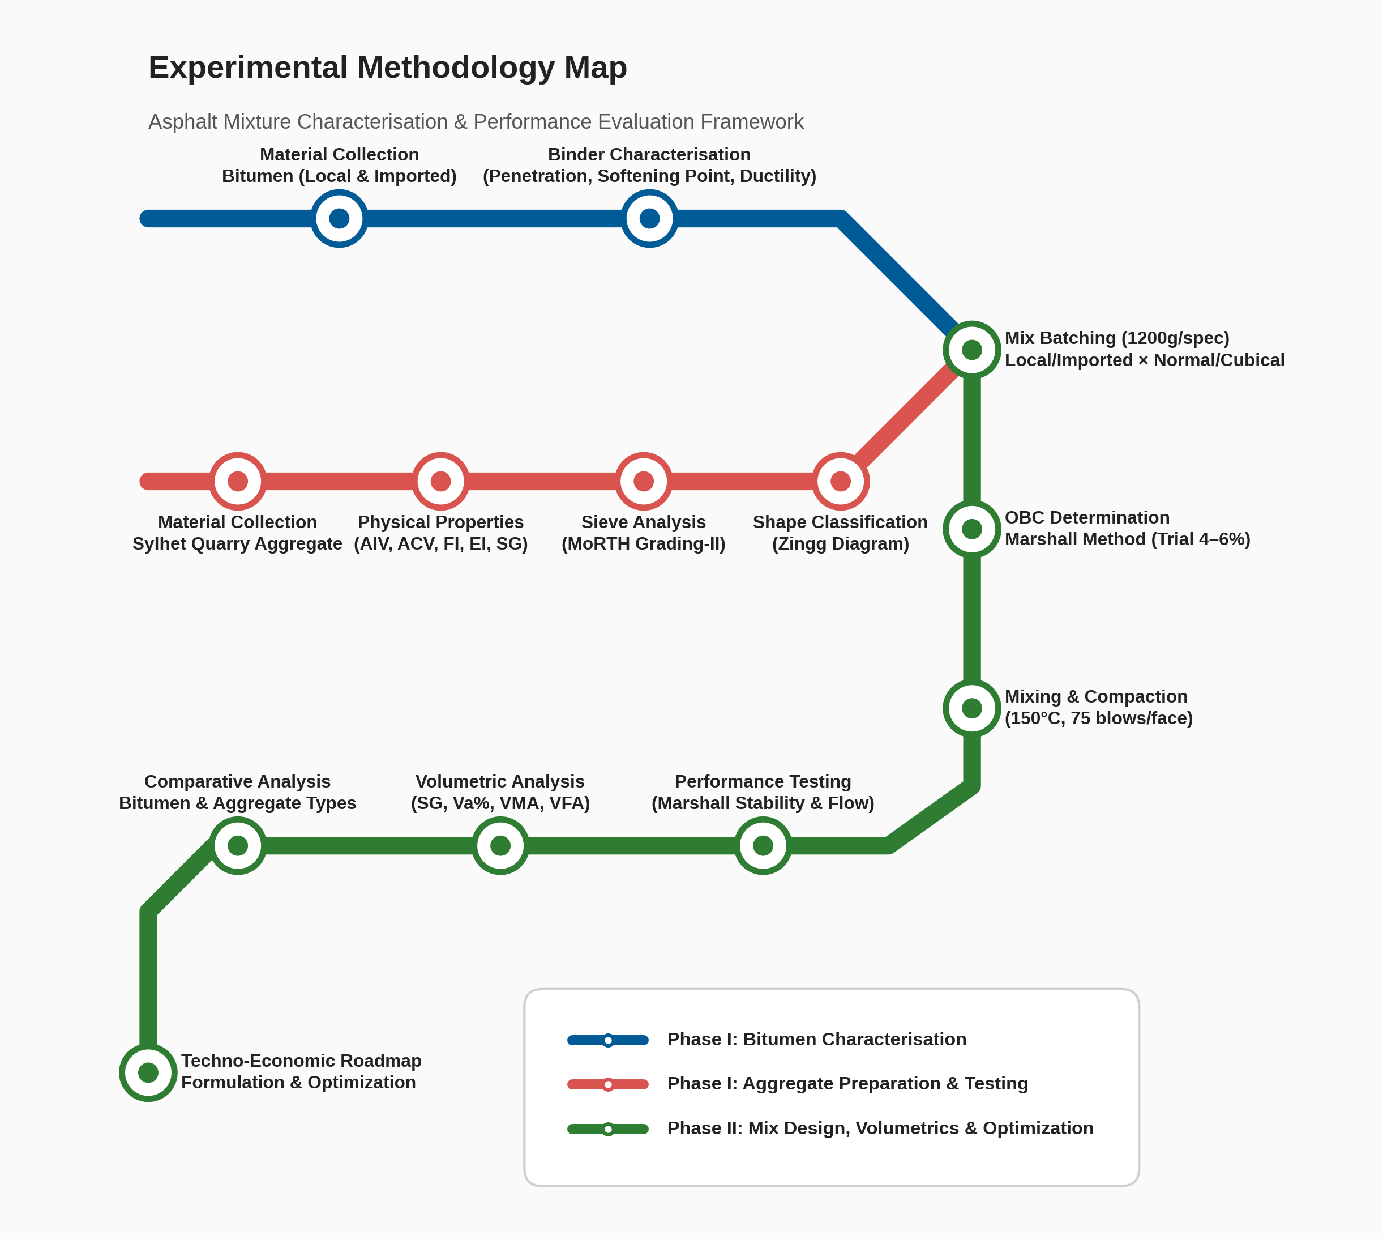
\includegraphics[width=0.85\textwidth]{graphics/methodology_flowchart.pdf}
    \caption{Flowchart of the experimental methodology adopted in this study.}
    \label{fig:flowchart}
\end{figure}

\subsection{Materials}

\subsubsection{Bitumen}

We used two sources of 60/70 penetration-grade bitumen in this study: (i) locally produced bitumen from Eastern Refinery Limited, Chittagong, Bangladesh, and (ii) imported low-cost bitumen bought from the open market. Both binders were tested according to the relevant ASTM standards. The tests included penetration at 25$^{\circ}$C (ASTM D5, Standard Test Method for Penetration of Bituminous Materials), softening point by the ring-and-ball method (ASTM D36, Standard Test Method for Softening Point of Bitumen), ductility at 25$^{\circ}$C (ASTM D113, Standard Test Method for Ductility of Asphalt Materials), kinematic viscosity (ASTM D2170, Standard Test Method for Kinematic Viscosity of Asphalts), specific gravity at 25$^{\circ}$C (ASTM D70, Standard Test Method for Density of Semi-Solid Asphalt Binder), and flash point by the Cleveland open cup method (ASTM D92, Standard Test Method for Flash and Fire Points). The properties of the local and imported bitumen are listed in Table~\ref{tab:local_bitumen} and Table~\ref{tab:imported_bitumen}.

\begin{table}[htbp]
    \centering
    \caption{Physical properties of local bitumen (Eastern Refinery, 60/70 grade).}
    \label{tab:local_bitumen}
    \begin{tabular}{@{}llc@{}}
        \toprule
        \textbf{Property} & \textbf{Test Standard} & \textbf{Specification} \\
        \midrule
        Penetration at 25$^{\circ}$C (dmm) & ASTM D5 & 60--70 \\
        Softening Point ($^{\circ}$C) & ASTM D36 & 49--56 \\
        Ductility at 25$^{\circ}$C (cm) & ASTM D113 & $\geq$75 \\
        Kinematic Viscosity at 135$^{\circ}$C (cSt) & ASTM D2170 & $\geq$300 \\
        Specific Gravity at 25$^{\circ}$C & ASTM D70 & 0.97--1.02 \\
        Flash Point ($^{\circ}$C) & ASTM D92 & $\geq$230 \\
        \bottomrule
    \end{tabular}
\end{table}

\begin{table}[htbp]
    \centering
    \caption{Physical properties of imported low-cost bitumen (60/70 grade).}
    \label{tab:imported_bitumen}
    \begin{tabular}{@{}llc@{}}
        \toprule
        \textbf{Property} & \textbf{Test Standard} & \textbf{Specification} \\
        \midrule
        Penetration at 25$^{\circ}$C (dmm) & ASTM D5 & 60--70 \\
        Softening Point ($^{\circ}$C) & ASTM D36 & 49--56 \\
        Ductility at 25$^{\circ}$C (cm) & ASTM D113 & $\geq$75 \\
        Kinematic Viscosity at 135$^{\circ}$C (cSt) & ASTM D2170 & $\geq$300 \\
        Specific Gravity at 25$^{\circ}$C & ASTM D70 & 0.97--1.02 \\
        Flash Point ($^{\circ}$C) & ASTM D92 & $\geq$230 \\
        \bottomrule
    \end{tabular}
\end{table}

\subsubsection{Aggregates}

Crushed stone aggregates were collected from a local quarry in the Sylhet region. We tested the aggregates for their physical and mechanical properties following the relevant standards. The tests performed were the Los Angeles Abrasion test, the Aggregate Impact Value (AIV) test, the Aggregate Crushing Value test, specific gravity, and water absorption. The results and the specification requirements are shown in Table~\ref{tab:agg_properties}.

\begin{table}[htbp]
    \centering
    \caption{Physical and mechanical properties of coarse aggregates.}
    \label{tab:agg_properties}
    \begin{tabular}{@{}llc@{}}
        \toprule
        \textbf{Property} & \textbf{Test Standard} & \textbf{Specification Limit} \\
        \midrule
        Los Angeles Abrasion Value (\%) & ASTM C131 & $\leq$30 \\
        Aggregate Impact Value (\%) & IS 2386 Part IV & $\leq$27 \\
        Aggregate Crushing Value (\%) & IS 2386 Part IV & $\leq$30 \\
        Specific Gravity (Coarse) & ASTM C127 & 2.5--2.9 \\
        Specific Gravity (Fine) & ASTM C128 & 2.5--2.9 \\
        Water Absorption (\%) & ASTM C127 & $\leq$2 \\
        Flakiness Index (\%) & IS 2386 Part I & $\leq$30 \\
        Elongation Index (\%) & IS 2386 Part I & $\leq$30 \\
        \bottomrule
    \end{tabular}
\end{table}

\subsubsection{Mineral Filler}

Stone dust was used as the mineral filler. We obtained the filler by collecting the fraction passing the 0.075\,mm (No.\,200) sieve from the same quarry source. The filler gradation met the requirements given in MoRTH Section 500.

\subsection{Aggregate Gradation and Blending}
\label{subsec:agg_gradation}

We designed the aggregate blend to conform to the Dense Bituminous Macadam (DBM) Grading-II specification from MoRTH Table 500-10. Sieve analysis identified four material fractions, which were blended in the following proportions to stay within the gradation envelope:

\begin{itemize}
    \item Material A: 19\,mm -- 12.5\,mm retained fraction (53\%)
    \item Material B: 12.5\,mm -- 2.36\,mm retained fraction (2\%)
    \item Material C: 2.36\,mm -- 0.075\,mm retained fraction (43\%)
    \item Material D: Passing 0.075\,mm, mineral filler (2\%)
\end{itemize}

The combined gradation and the MoRTH specification limits are given in Table~\ref{tab:gradation}. Figure~\ref{fig:gradation} shows the gradation curve plotted against the upper and lower specification boundaries.

\begin{table}[htbp]
    \centering
    \caption{Combined aggregate gradation for DBM Grading-II (MoRTH Table 500-10).}
    \label{tab:gradation}
    \begin{tabular}{@{}cccc@{}}
        \toprule
        \textbf{IS Sieve Size (mm)} & \textbf{Lower Limit (\%)} & \textbf{Upper Limit (\%)} & \textbf{Trial Mix (\%)} \\
        \midrule
        26.5  & 100 & 100 & 100 \\
        19    & 90  & 100 & 98  \\
        13.2  & 71  & 95  & 82  \\
        9.5   & 56  & 80  & 64  \\
        4.75  & 38  & 54  & 46  \\
        2.36  & 28  & 42  & 37  \\
        0.3   & 7   & 21  & 16  \\
        0.075 & 4   & 8   & 6   \\
        \bottomrule
    \end{tabular}
\end{table}

\begin{figure}[htbp]
    \centering
    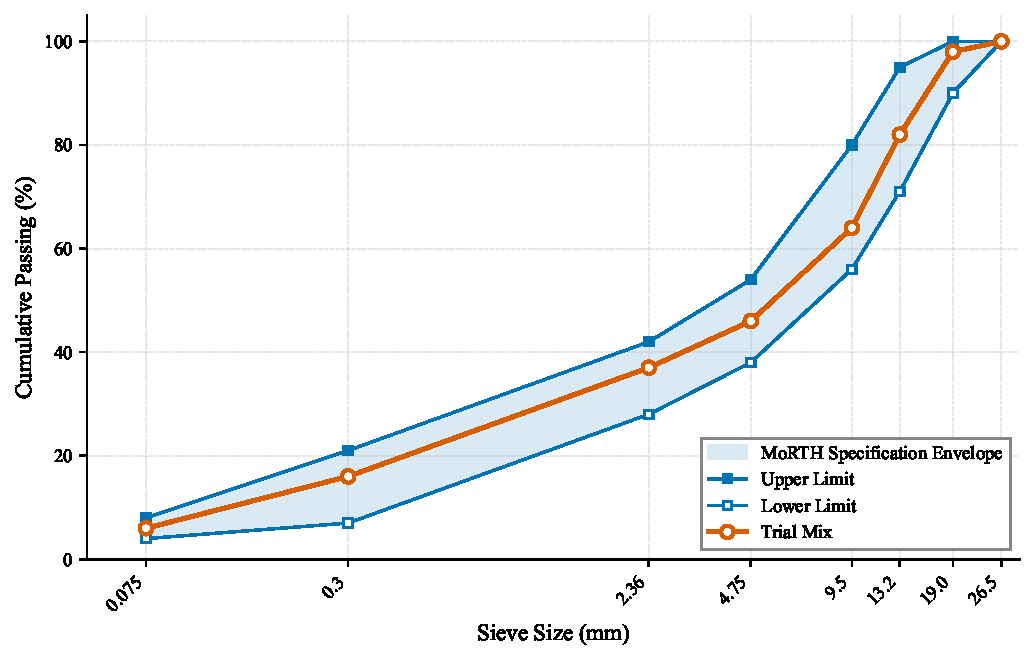
\includegraphics[width=0.9\textwidth]{graphics/gradation_curve.pdf}
    \caption{Aggregate gradation curve for DBM Grading-II with MoRTH specification limits.}
    \label{fig:gradation}
\end{figure}

\subsection{Aggregate Shape Classification}

We characterised the shape of the coarse aggregates retained on the 12.5\,mm sieve (Material A fraction: 19 to 12.5\,mm) using the Zingg diagram classification. For each particle, three orthogonal dimensions were measured with Vernier calipers: the longest diameter ($d_L$), the intermediate diameter ($d_I$), and the shortest diameter ($d_S$). From these measurements, two dimensionless ratios were calculated:

\begin{equation}
    \text{Elongation Ratio} = \frac{d_I}{d_L}
    \label{eq:elongation}
\end{equation}

\begin{equation}
    \text{Flatness Ratio} = \frac{d_S}{d_I}
    \label{eq:flatness}
\end{equation}

Using a threshold value of $2/3$ for each ratio, we classified the aggregate particles into four shape categories according to the Zingg diagram~\cite{teja2020effect}: Cubical (Elongation Ratio $\geq 2/3$ and Flatness Ratio $\geq 2/3$), Rod (Elongation Ratio $< 2/3$ and Flatness Ratio $\geq 2/3$), Disk (Elongation Ratio $\geq 2/3$ and Flatness Ratio $< 2/3$), and Blade (Elongation Ratio $< 2/3$ and Flatness Ratio $< 2/3$). The Zingg classification scheme is shown in Figure~\ref{fig:zingg}.

The particles identified as cubical were separated by hand and set aside for Mix-3 and Mix-4, where they replaced 20\% of the coarse aggregate (Material A) fraction by weight.

\begin{figure}[htbp]
    \centering
    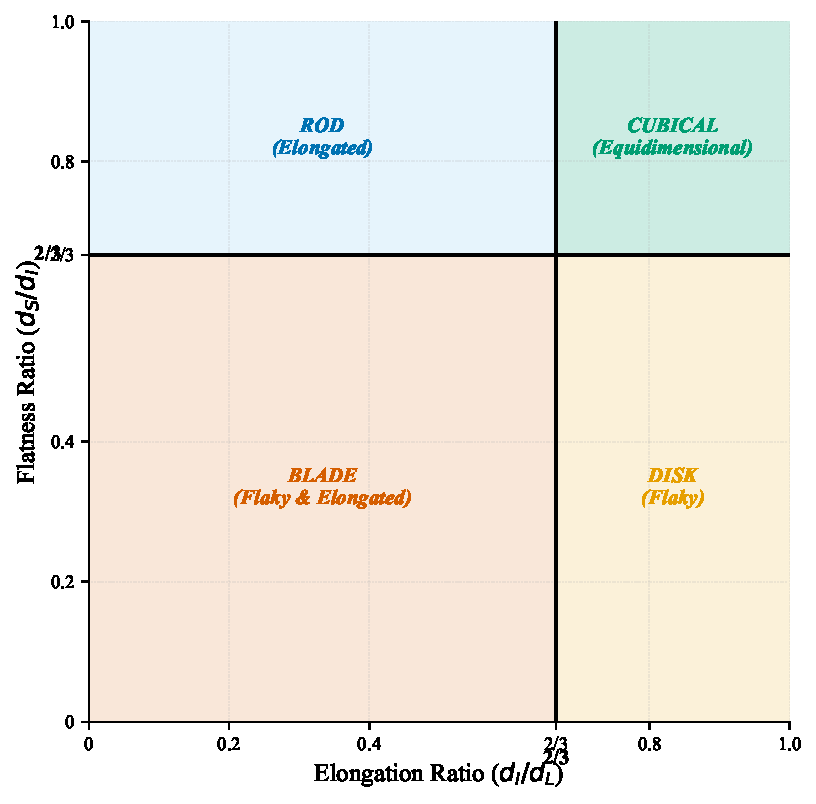
\includegraphics[width=0.7\textwidth]{graphics/zingg_diagram.pdf}
    \caption{Zingg diagram for aggregate shape classification based on elongation ratio and flatness ratio.}
    \label{fig:zingg}
\end{figure}

\subsection{Mix Design}

\subsubsection{Mix Combinations}

We designed four mix combinations to study how bitumen source and aggregate shape together affect the performance of bituminous mixes. Table~\ref{tab:mix_matrix} shows the experimental matrix.

\begin{table}[htbp]
    \centering
    \caption{Experimental mix design matrix.}
    \label{tab:mix_matrix}
    \begin{tabular}{@{}clll@{}}
        \toprule
        \textbf{Mix} & \textbf{Bitumen Source} & \textbf{Aggregate Type} & \textbf{Purpose} \\
        \midrule
        Mix-1 & Local (Eastern Refinery) & Natural (as-received) & Control + OBC determination \\
        Mix-2 & Imported (low-cost) & Natural (as-received) & Imported bitumen control \\
        Mix-3 & Local (Eastern Refinery) & 20\% cubical replacement & Shape effect (local) \\
        Mix-4 & Imported (low-cost) & 20\% cubical replacement & Shape effect (imported) \\
        \bottomrule
    \end{tabular}
\end{table}

\subsubsection{Specimen Preparation}

Each specimen had a total batch weight of 1200\,g. Following the MoRTH specifications for Dense Bituminous Macadam (DBM) Grading-II, the material proportions were set as described in Section~\ref{subsec:agg_gradation}: 55\% coarse aggregate, 43\% fine aggregate, and 2\% mineral filler. We heated the aggregates in an oven at 150 to 170$^{\circ}$C before mixing. The bitumen was heated separately to 150$^{\circ}$C so it would reach the right mixing viscosity. Once both were at the correct temperature, we combined the aggregate and the bitumen (at the optimum binder content) and mixed them thoroughly until every particle was coated.

The mix was then placed into a preheated Marshall mould (101.6\,mm diameter) and rodded with a spatula to remove trapped air. We applied 75 blows to each face using a standard Marshall hammer, satisfying the MoRTH criteria for heavy-traffic roads~\cite{rajkumar2018experimental}. The compacted specimens cooled completely to ambient temperature prior to extraction.

\subsubsection{Optimum Binder Content Determination}

We determined the Optimum Binder Content (OBC) using Mix-1 (local bitumen with natural aggregates), which was the control mix. Five trial bitumen contents were tested: 4.0\%, 4.5\%, 5.0\%, 5.5\%, and 6.0\% by weight of the total mix. For each bitumen content, three replicate specimens were made and tested for Marshall stability, flow, bulk specific gravity, and air voids.

We established the OBC by averaging the binder contents that yielded maximum Marshall stability, peak bulk specific gravity, and the target 4\% air void threshold. This calculation produced an optimal content of \textbf{5.0\%}. We then used this value for all the remaining mixes (Mix-2, Mix-3, and Mix-4) so that the comparison would be on an equal footing.

\subsection{Testing Programme}

\subsubsection{Marshall Stability and Flow Test}

The Marshall stability and flow test followed ASTM D6927 / AASHTO T245. For each of the four mix combinations, we prepared three replicate specimens at the 5.0\% OBC. Before testing, the specimens were placed in a water bath at 60$^{\circ}$C for 30 to 40 minutes. We then recorded the Marshall stability (the maximum load the specimen could carry, in kN) and the flow value (the deformation at maximum load, in mm).

\subsubsection{Volumetric Analysis}

We also determined the volumetric properties of the compacted specimens for all four mixes. The following parameters were calculated:

\begin{itemize}
    \item Bulk Specific Gravity ($G_{mb}$)
    \item Air Voids ($V_a$, \%)
    \item Voids in Mineral Aggregate (VMA, \%)
    \item Voids Filled with Bitumen (VFB, \%)
\end{itemize}

\subsection{Summary of Test Matrix}

Table~\ref{tab:test_matrix} summarises the test matrix. In total, 12 Marshall specimens were prepared across the four mix combinations for the performance tests at the optimum binder content.

\begin{table}[htbp]
    \centering
    \caption{Summary of the experimental test matrix.}
    \label{tab:test_matrix}
    \begin{tabular}{@{}lccc@{}}
        \toprule
        \textbf{Test} & \textbf{Specimens per Mix} & \textbf{Number of Mixes} & \textbf{Total Specimens} \\
        \midrule
        Marshall Stability \& Flow & 3 & 4 & 12 \\
        \midrule
        \textbf{Grand Total} & & & \textbf{12} \\
        \bottomrule
    \end{tabular}
\end{table}


\section{Results and Discussion}

\subsection{Properties of Aggregates}

We tested the physical and mechanical properties of the coarse aggregates from the Sylhet quarry and compared them against the specification limits. Since we used a single source of crushed stone, no cross-variant comparison was needed; the results are simply checked against the maximum allowable values.

Figure~\ref{fig:agg_properties} shows the results. The Aggregate Impact Value (AIV) was 18\% and the Aggregate Crushing Value (ACV) was 20\%, both well within the maximum limits of 27\% and 30\%. The Flakiness Index came out at 15\% and the Elongation Index at 23\%, both below the 30\% maximum. This means the aggregates, even before any manual shape-sorting, already met the shape requirements.

\begin{figure}[htbp]
    \centering
    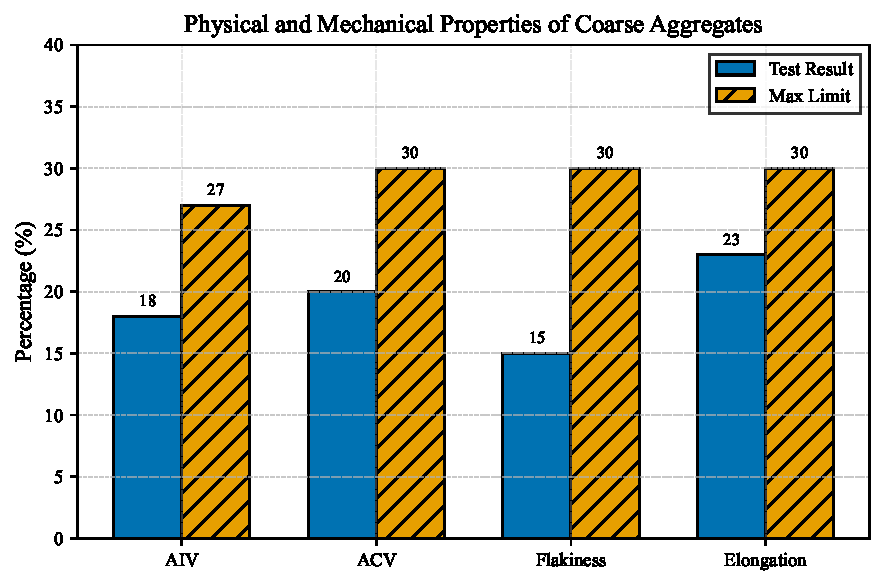
\includegraphics[width=0.7\textwidth]{graphics/aggregate_properties.pdf}
    \caption{Physical and mechanical properties of coarse aggregates compared with maximum specification limits.}
    \label{fig:agg_properties}
\end{figure}

\subsection{Properties of Bituminous Binders}

Because Bangladesh's own bitumen production cannot always meet the country's demand, imported bitumen fills the gap. The trouble is that these imported binders vary in quality, and that can lead to problems like rutting and thermal cracking. To see exactly how the local and imported bitumen compare, we tested both and plotted the results.

Figure~\ref{fig:bitumen_properties} shows the comparison. The local ERL bitumen had a higher specific gravity (1.023) than the imported bitumen (0.99). Its softening point was also higher: 52$^{\circ}$C versus 41$^{\circ}$C for the imported binder, which means the local bitumen resists high-temperature deformation better.

The flash point and fire point of the local bitumen (255$^{\circ}$C and 312$^{\circ}$C) were both higher than the imported binder's values (218$^{\circ}$C and 253$^{\circ}$C). Ductility was 112\,cm for the local bitumen and 91\,cm for the imported one. Across all the physical and rheological properties we tested, the local ERL bitumen met or exceeded the requirements.

\begin{figure}[htbp]
    \centering
    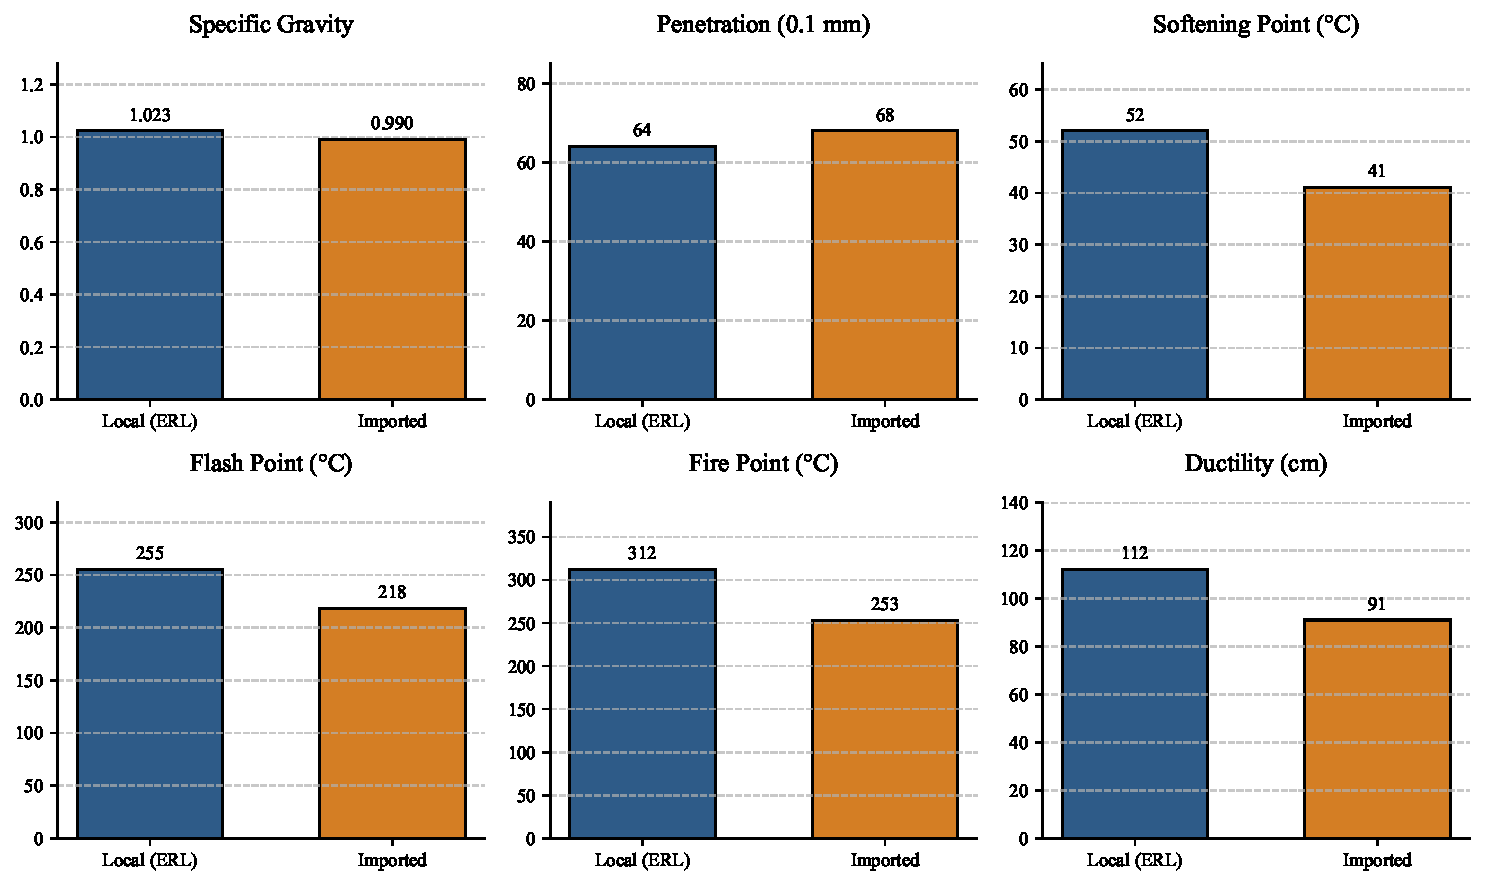
\includegraphics[width=.85\textwidth]{graphics/bitumen_properties.pdf}
    \caption{Graphical comparison of physical properties between local (ERL) and imported low-cost bitumen.}
    \label{fig:bitumen_properties}
\end{figure}

\noindent\textbf{Regional Comparative Assessment (South Asia):}
We also compared both binders against the highway specifications of neighbouring South Asian countries (India, Pakistan, and Nepal). The details are in Table~\ref{tab:regional_comparison} and Figure~\ref{fig:bitumen_regional_comparison}. The local ERL bitumen, with a softening point of $52^{\circ}\text{C}$, passes the requirements of Pakistan's NHA ($48$ to $56^{\circ}\text{C}$), Nepal's DOR ($48$ to $56^{\circ}\text{C}$), and India's MORT\&H (minimum $47^{\circ}\text{C}$). The imported bitumen had a softening point of only $41^{\circ}\text{C}$, which falls below the minimum set by all of these regional authorities.

The imported bitumen's flash point ($218^{\circ}\text{C}$) also fails to meet the $232^{\circ}\text{C}$ minimum safety threshold used in Bangladesh, India, Nepal, and Pakistan. The local ERL bitumen's flash point of $255^{\circ}\text{C}$ comfortably exceeds this threshold. The imported bitumen we tested does not meet the regional specifications for use in flexible pavements.

\begin{table}[htbp]
    \centering
    \caption{Comparative analysis of physical properties between experimental bitumen and South Asian standards.}
    \label{tab:regional_comparison}
    \renewcommand{\arraystretch}{1.3}
    \resizebox{\textwidth}{!}{%
    \begin{tabular}{@{}lccccccc@{}}
        \toprule
        \multirow{2}{*}{\textbf{Property}} & \multicolumn{2}{c}{\textbf{Experimental Data}} & \multicolumn{4}{c}{\textbf{National Specifications (60/70 Grade)}} & \multirow{2}{*}{\textbf{Standard}} \\
        \cmidrule(lr){2-3} \cmidrule(lr){4-7}
        & \textbf{Local (ERL)} & \textbf{Imported} & \textbf{RHD (BD)} & \textbf{MORT\&H (IN)} & \textbf{DOR (NP)} & \textbf{NHA (PK)} & \\
        \midrule
        Penetration (dmm) & 64 & 68 & 60--70 & 60--70 & 60--70 & 60--70 & ASTM D5 \\
        Softening Point ($^\circ$C) & 52 & \textbf{41} & 48--56 & 47--55 & 48--56 & 48--56 & ASTM D36 \\
        Ductility (cm) & 112 & \textbf{91} & $\geq$100 & $\geq$75 & $\geq$100 & $\geq$100 & ASTM D113 \\
        Flash Point ($^\circ$C) & 255 & \textbf{218} & $\geq$232 & $\geq$232 & $\geq$232 & $\geq$232 & ASTM D92 \\
        Specific Gravity & 1.023 & \textbf{0.990} & 1.01--1.06 & 1.01--1.06 & 1.01--1.06 & 1.01--1.06 & ASTM D70 \\
        \bottomrule
        \multicolumn{8}{@{}l@{}}{\small Note: Bold values indicate the imported bitumen failed to meet the specified minimum regional requirements.} \\
    \end{tabular}%
    }
\end{table}

\begin{figure}[htbp]
    \centering
    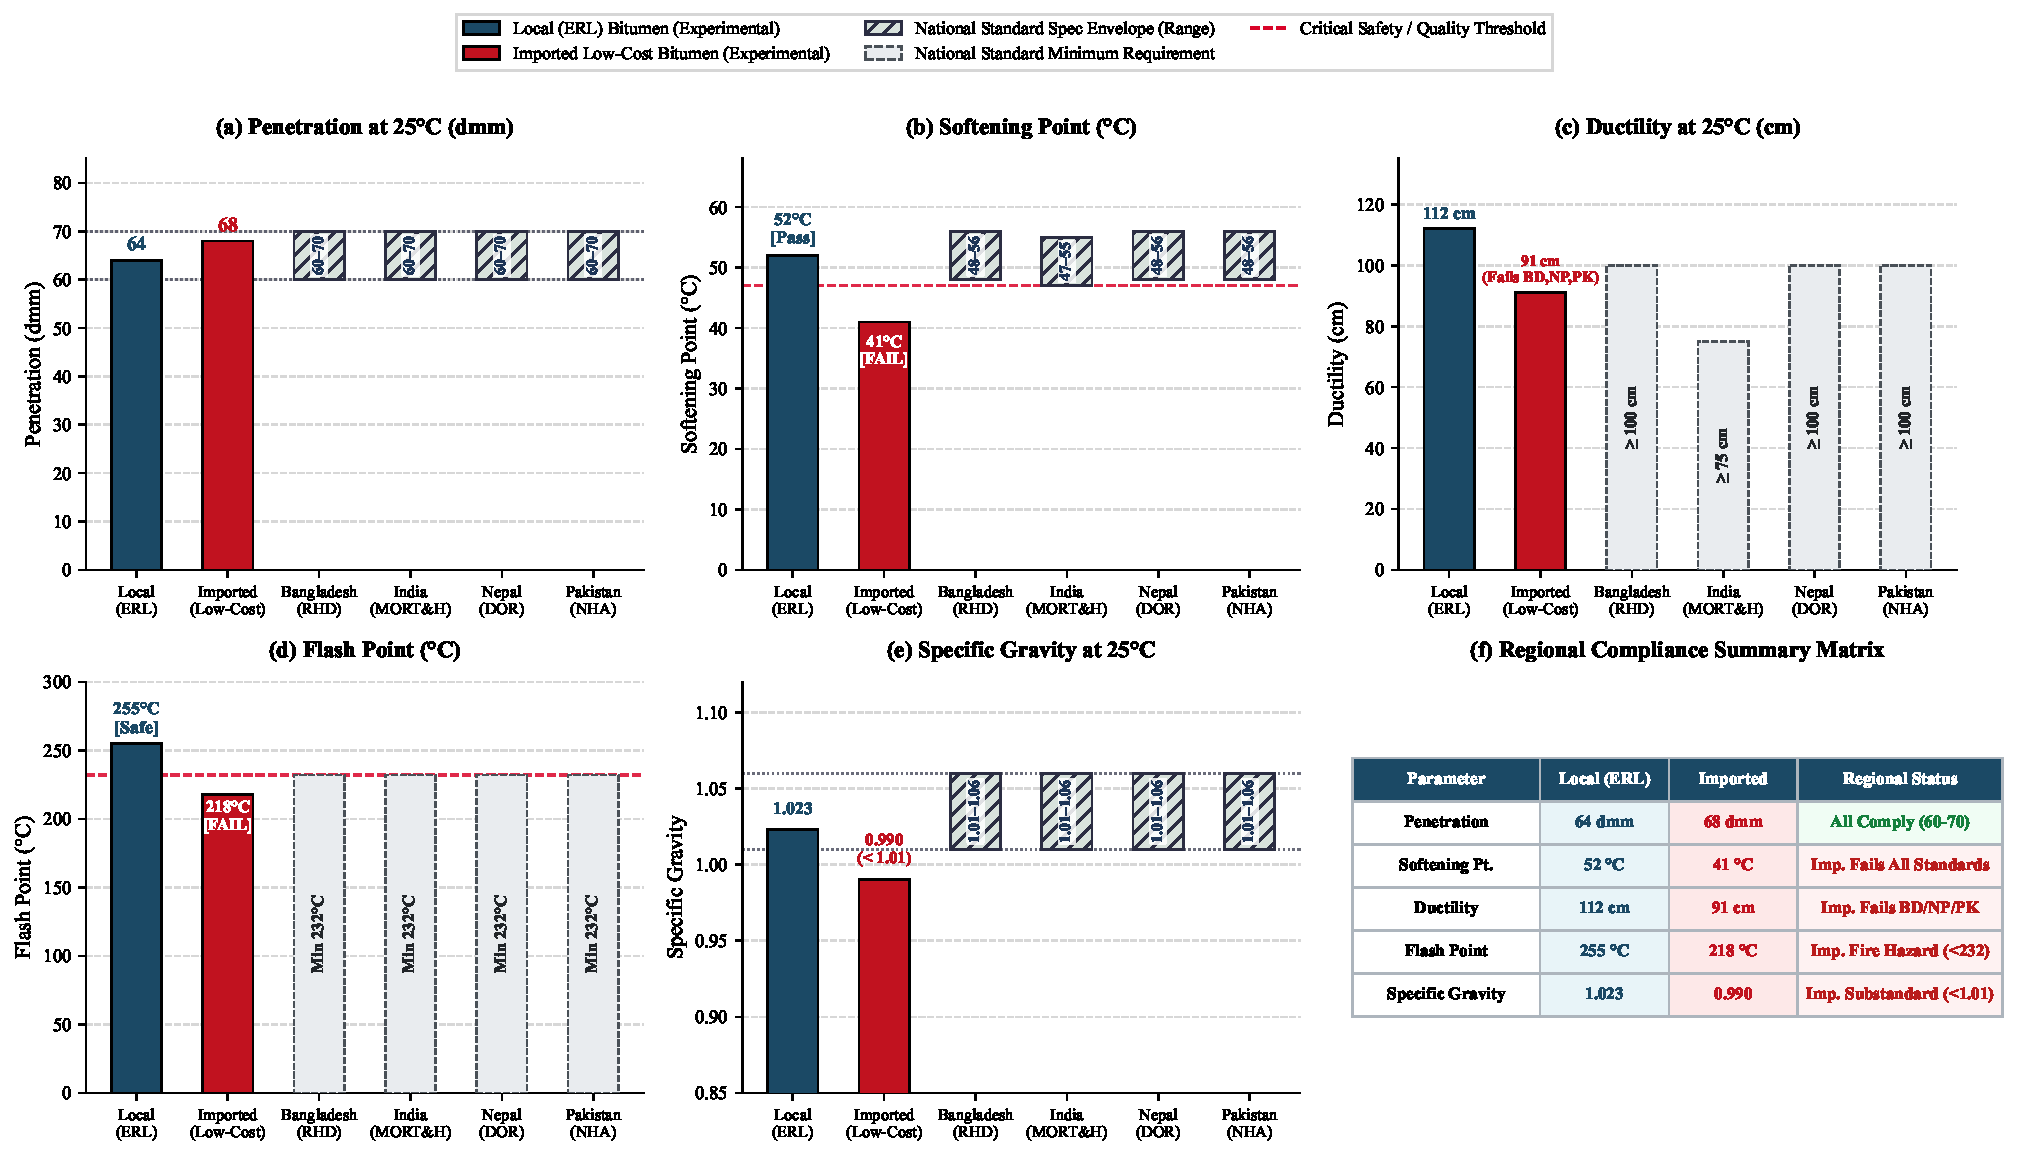
\includegraphics[width=\textwidth]{graphics/bitumen_regional_comparison.pdf}
    \caption{Comparative analysis of experimental physical properties of local (ERL) and imported low-cost bitumen against national highway specifications of South Asian countries (Bangladesh RHD, India MORT\&H, Nepal DOR, and Pakistan NHA).}
    \label{fig:bitumen_regional_comparison}
\end{figure}

\clearpage
\subsection{Determination of Optimum Binder Content}

We used the Marshall mix design method to find the Optimum Binder Content (OBC) for both the local and imported bitumen. Specimens were prepared at asphalt contents of 4.0\%, 4.5\%, 5.0\%, 5.5\%, and 6.0\%. For each content, we measured the volumetric properties (air voids, VMA, VFA) and mechanical properties (Marshall stability, flow, and unit weight) to work out the best mix proportions.

Table~\ref{tab:obc_data} and Figure~\ref{fig:obc_determination} show the results. For both binders, stability peaked at a certain asphalt content and then dropped off at higher contents, while the flow value kept increasing. The target air void content ($V_a$) of 4.0\%, which is the standard criterion for heavy-traffic pavements, corresponded to an asphalt content of about 5.0\% for both the local and imported mixes. At 5.0\%, the other parameters (VMA, VFA, and unit weight) all fell within the RHD specification limits. So we adopted 5.0\% as the OBC for the rest of the comparative tests.

The volumetric properties of the Marshall specimens were calculated using the following equations:
\begin{align}
    G_{mb} &= \frac{W_a}{W_{ssd} - W_w} \\
    G_{mm} &= \frac{P_{mm}}{\frac{P_s}{G_{se}} + \frac{P_b}{G_b}} \\
    P_s &= 100 - P_b \\
    P_{mm} &= 100 \\
    G_{se} &= \frac{P_{mm} - P_b}{\frac{P_{mm}}{G_{mm}} - \frac{P_b}{G_b}} \\
    G_{sb} &= \frac{P_1 + P_2 + P_3}{\frac{P_1}{G_1} + \frac{P_2}{G_2} + \frac{P_3}{G_3}} \\
    V_a (\%) &= 100 \times \frac{G_{mm} - G_{mb}}{G_{mm}} \\
    \text{VMA} (\%) &= 100 - \frac{G_{mb} \times P_s}{G_{sb}} \\
    \text{VFA} (\%) &= \frac{\text{VMA} - V_a}{\text{VMA}} \times 100
\end{align}
where $W_a$ represents the dry mass in air, $W_{ssd}$ denotes the saturated surface-dry mass, and $W_w$ is the mass submerged in water. $P_b$ and $P_s$ refer to the binder and aggregate percentages of the total mix mass, respectively. $G_b$ stands for the specific gravity of the bitumen, $G_{se}$ is the effective aggregate specific gravity, and $G_{sb}$ indicates the bulk specific gravity of the combined aggregates (where $P_1, P_2, P_3$ and $G_1, G_2, G_3$ specify the proportions and specific gravities of each aggregate fraction). Finally, $G_{mm}$ defines the theoretical maximum mixture specific gravity, and $G_{mb}$ signifies the bulk specific gravity of the densified Marshall specimen.

\begin{table}[htbp]
    \centering
    \caption{Marshall mix design properties for Optimum Binder Content determination.}
    \label{tab:obc_data}
    \resizebox{\textwidth}{!}{
    \begin{threeparttable}
    \begin{tabular}{lccccccccccccccccc}
        \toprule
        \textbf{Bitumen Type} & \textbf{AC} & \textbf{$W_a$} & \textbf{$W_w$} & \textbf{$W_{ssd}$} & \textbf{$G_{mb}$} & \textbf{$\gamma$} & \textbf{$G_{mm}$} & \textbf{$P_s$} & \textbf{$G_{sb}$} & \textbf{$V_a$} & \textbf{VMA} & \textbf{VFA} & \textbf{$H$} & \textbf{CF} & \textbf{$S_{obs}$} & \textbf{$S_{cor}$} & \textbf{$F$} \\
        \midrule
        \multirow{5}{*}{\textbf{Local (ERL)}} 
        & 4.0 & 1176.5 & 677.4 & 1181.2 & 2.330 & 145.72 & 2.520 & 96.0 & 2.684 & 7.54 & 16.66 & 54.75 & 65.0 & 0.932 & 1946 & 1813.67 & 9.5 \\
        & 4.5 & 1216.6 & 704.7 & 1230.2 & 2.315 & 144.46 & 2.501 & 95.5 & 2.684 & 7.44 & 17.44 & 57.81 & 65.0 & 0.932 & 2625 & 2446.50 & 9.0 \\
        & 5.0 & 1202.3 & 696.9 & 1206.3 & 2.360 & 147.28 & 2.482 & 95.0 & 2.684 & 4.92 & 16.47 & 70.15 & 63.5 & 1.000 & 2500 & 2500.00 & 10.0 \\
        & 5.5 & 1221.2 & 715.6 & 1222.3 & 2.410 & 150.38 & 2.464 & 94.5 & 2.684 & 2.19 & 15.15 & 85.54 & 64.3 & 0.950 & 2517 & 2438.60 & 11.0 \\
        & 6.0 & 1230.6 & 722.4 & 1231.3 & 2.418 & 150.89 & 2.445 & 94.0 & 2.684 & 1.10 & 15.32 & 92.79 & 65.0 & 0.932 & 2273 & 2118.40 & 14.0 \\
        \midrule
        \multirow{5}{*}{\textbf{Imported}} 
        & 4.0 & 1199.5 & 690.1 & 1204.2 & 2.333 & 145.58 & 2.520 & 96.0 & 2.684 & 7.42 & 16.55 & 55.17 & 64.5 & 0.946 & 1452 & 1373.81 & 10.0 \\
        & 4.5 & 1205.9 & 691.5 & 1210.7 & 2.323 & 144.96 & 2.501 & 95.5 & 2.684 & 7.12 & 17.35 & 58.97 & 64.6 & 0.944 & 1133 & 1069.42 & 11.0 \\
        & 5.0 & 1206.7 & 701.6 & 1208.6 & 2.380 & 148.51 & 2.482 & 95.0 & 2.684 & 4.11 & 15.76 & 73.92 & 63.4 & 1.003 & 1909 & 1913.51 & 11.0 \\
        & 5.5 & 1225.7 & 715.8 & 1226.8 & 2.399 & 149.70 & 2.464 & 94.5 & 2.684 & 2.64 & 15.53 & 83.01 & 63.6 & 0.992 & 2045 & 2028.64 & 12.0 \\
        & 6.0 & 1200.0 & 708.1 & 1201.5 & 2.432 & 151.76 & 2.445 & 94.0 & 2.684 & 0.53 & 14.83 & 96.11 & 65.1 & 0.960 & 2274 & 2182.67 & 15.0 \\
        \bottomrule
    \end{tabular}
    \begin{tablenotes}
        \small
        \item \textit{Note:} AC = Asphalt Content (\%); $W_a$ = Specimen weight in air (g); $W_w$ = Specimen weight in water (g); $W_{ssd}$ = Saturated surface dry weight (g); $G_{mb}$ = Bulk specific gravity; $\gamma$ = Unit weight (lb/cft); $G_{mm}$ = Maximum specific gravity; $P_s$ = Percent of aggregate (\%); $G_{sb}$ = Bulk specific gravity of aggregate; $V_a$ = Air voids (\%); VMA = Voids in mineral aggregate (\%); VFA = Voids filled with asphalt (\%); $H$ = Specimen height (mm); CF = Correction factor; $S_{obs}$ = Observed stability (lbs); $S_{cor}$ = Corrected stability (lbs); $F$ = Flow (0.25\,mm).
    \end{tablenotes}
    \end{threeparttable}
    }
\end{table}

\begin{figure}[H]
    \centering
    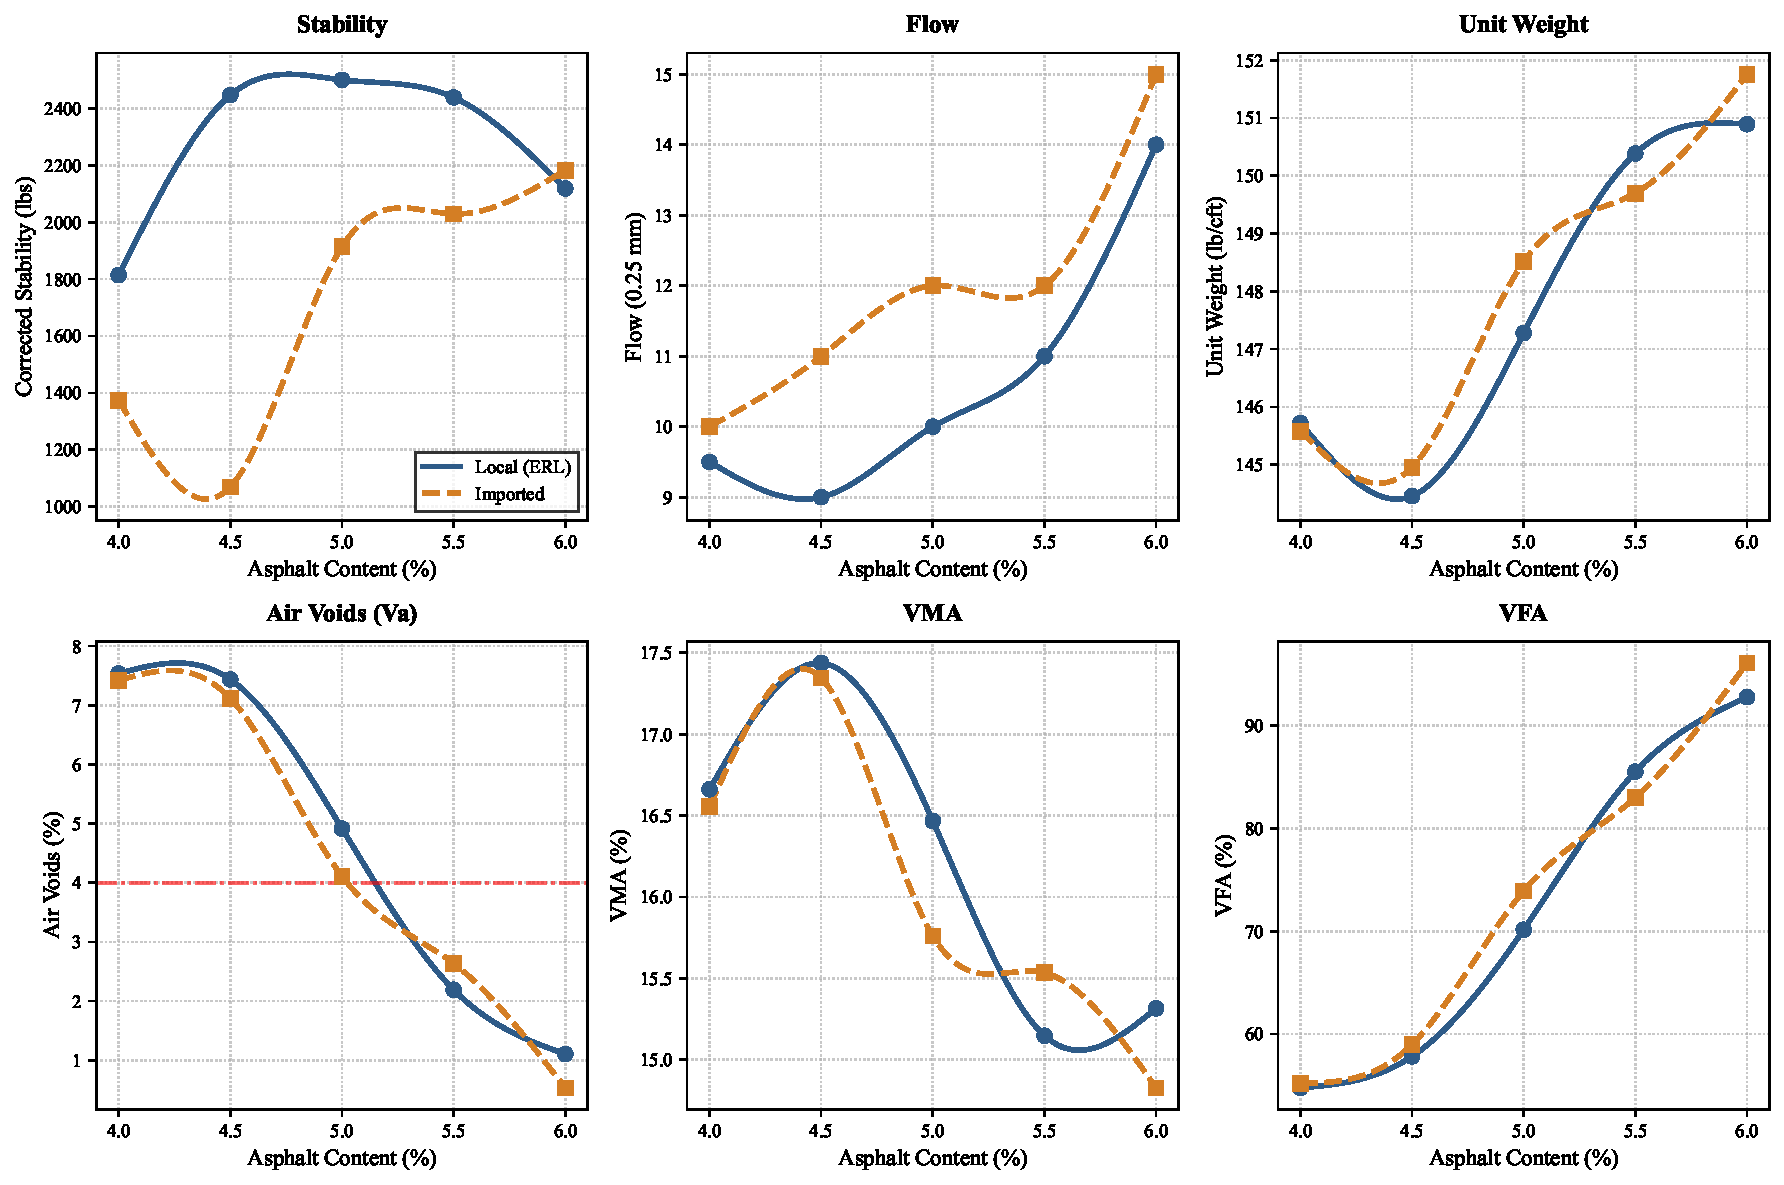
\includegraphics[width=\textwidth]{graphics/obc_determination.pdf}
    \caption{Marshall mix design properties across varying asphalt contents for Optimum Binder Content (OBC) determination.}
    \label{fig:obc_determination}
\end{figure}

\subsection{Comparative Analysis of Bituminous Mixtures}

With the OBC fixed at 5.0\%, we evaluated the four mix combinations for structural capacity, rutting susceptibility, and long-term cost implications. Table~\ref{tab:mix_data} presents the raw mechanical and volumetric data. Figure~\ref{fig:mix_comparison} visualises the stark interaction between the bitumen source and the inclusion of shape-sorted cubical aggregates.

\begin{table}[htbp]
    \centering
    \caption{Comparative Marshall properties of the four bituminous mix variants evaluated at 5.0\% OBC.}
    \label{tab:mix_data}
    \resizebox{\textwidth}{!}{
    \begin{threeparttable}
    \begin{tabular}{lccccccccccccccccc}
        \toprule
        \textbf{Variant} & \textbf{OBC} & \textbf{$W_a$} & \textbf{$W_w$} & \textbf{$W_{ssd}$} & \textbf{$G_{mb}$} & \textbf{$\gamma$} & \textbf{$G_{mm}$} & \textbf{$P_s$} & \textbf{$G_{sb}$} & \textbf{$V_a$} & \textbf{VMA} & \textbf{VFA} & \textbf{$H$} & \textbf{CF} & \textbf{$S_{obs}$} & \textbf{$S_{cor}$} & \textbf{$F$} \\
        \midrule
        Local + Normal & 5.0 & 1168.9 & 688.5 & 1176.0 & 2.398 & 149.64 & 2.479 & 95.0 & 2.680 & 3.27 & 15.00 & 78.20 & 61.9 & 1.040 & 1883 & 1958.81 & 10.0 \\
        Imp + Normal & 5.0 & 1176.8 & 679.7 & 1181.0 & 2.348 & 146.52 & 2.469 & 95.0 & 2.680 & 4.90 & 16.77 & 70.78 & 64.6 & 0.994 & 1126 & 1119.40 & 17.0 \\
        Local + 20\% Cubical & 5.0 & 1180.2 & 684.3 & 1186.0 & 2.350 & 146.64 & 2.479 & 95.0 & 2.680 & 5.20 & 16.70 & 68.86 & 60.3 & 1.090 & 2744 & 2990.55 & 8.5 \\
        Imp + 20\% Cubical & 5.0 & 1250.3 & 733.2 & 1253.0 & 2.405 & 150.07 & 2.469 & 95.0 & 2.680 & 2.59 & 14.93 & 82.65 & 65.1 & 0.960 & 2156 & 2070.13 & 12.0 \\
        \bottomrule
    \end{tabular}
    \begin{tablenotes}
        \small
        \item \textit{Note:} See Table~\ref{tab:obc_data} for column abbreviations. OBC = Optimum Binder Content (\%).
    \end{tablenotes}
    \end{threeparttable}
    }
\end{table}

\textbf{A. Overall Performance Assessment:}

We looked at all four mixes across both structural and volumetric parameters. Figure~\ref{fig:performance_assessment} shows Marshall stability, flow value, unit weight, air voids ($V_a$), voids in mineral aggregate (VMA), and voids filled with asphalt (VFA) for each mix. The data in Table~\ref{tab:mix_data} show that the binder source and the aggregate shape interact in ways that matter.

Looking at the volumetric side first: how the aggregate particles arrange themselves affects how well the mix compacts. The two control mixes with normal aggregates (Mix-1 and Mix-2) had air voids within standard limits ($3.27\%$ and $4.90\%$) and enough VMA to be durable. But when we added $20\%$ cubical aggregates, the volumetric response depended on which bitumen was used. With imported bitumen and cubical aggregates (Mix-4), the mix became very dense, with air voids dropping to just $2.59\%$ and VFA reaching $82.65\%$. In a subtropical monsoon climate, air voids that low raise the risk of binder bleeding and plastic flow when the pavement is loaded by traffic~\cite{imran2025developing}.

The local ERL bitumen combined with $20\%$ cubical aggregates (Mix-3) told a different story. It had a VMA of $16.70\%$, which leaves enough room for the binder film, while keeping air voids at $5.20\%$. As Figure~\ref{fig:performance_assessment} shows, this volumetric balance went hand-in-hand with higher shear resistance: the Marshall stability of this mix was $2990.55$\,lbs. The unit weight data also point to better densification and stronger aggregate interlock with the cubical particles. What Mix-3 shows is that it is possible to boost structural capacity without sacrificing the volumetric proportions needed for long-term fatigue life and rutting resistance.

\begin{figure}[H]
    \centering
    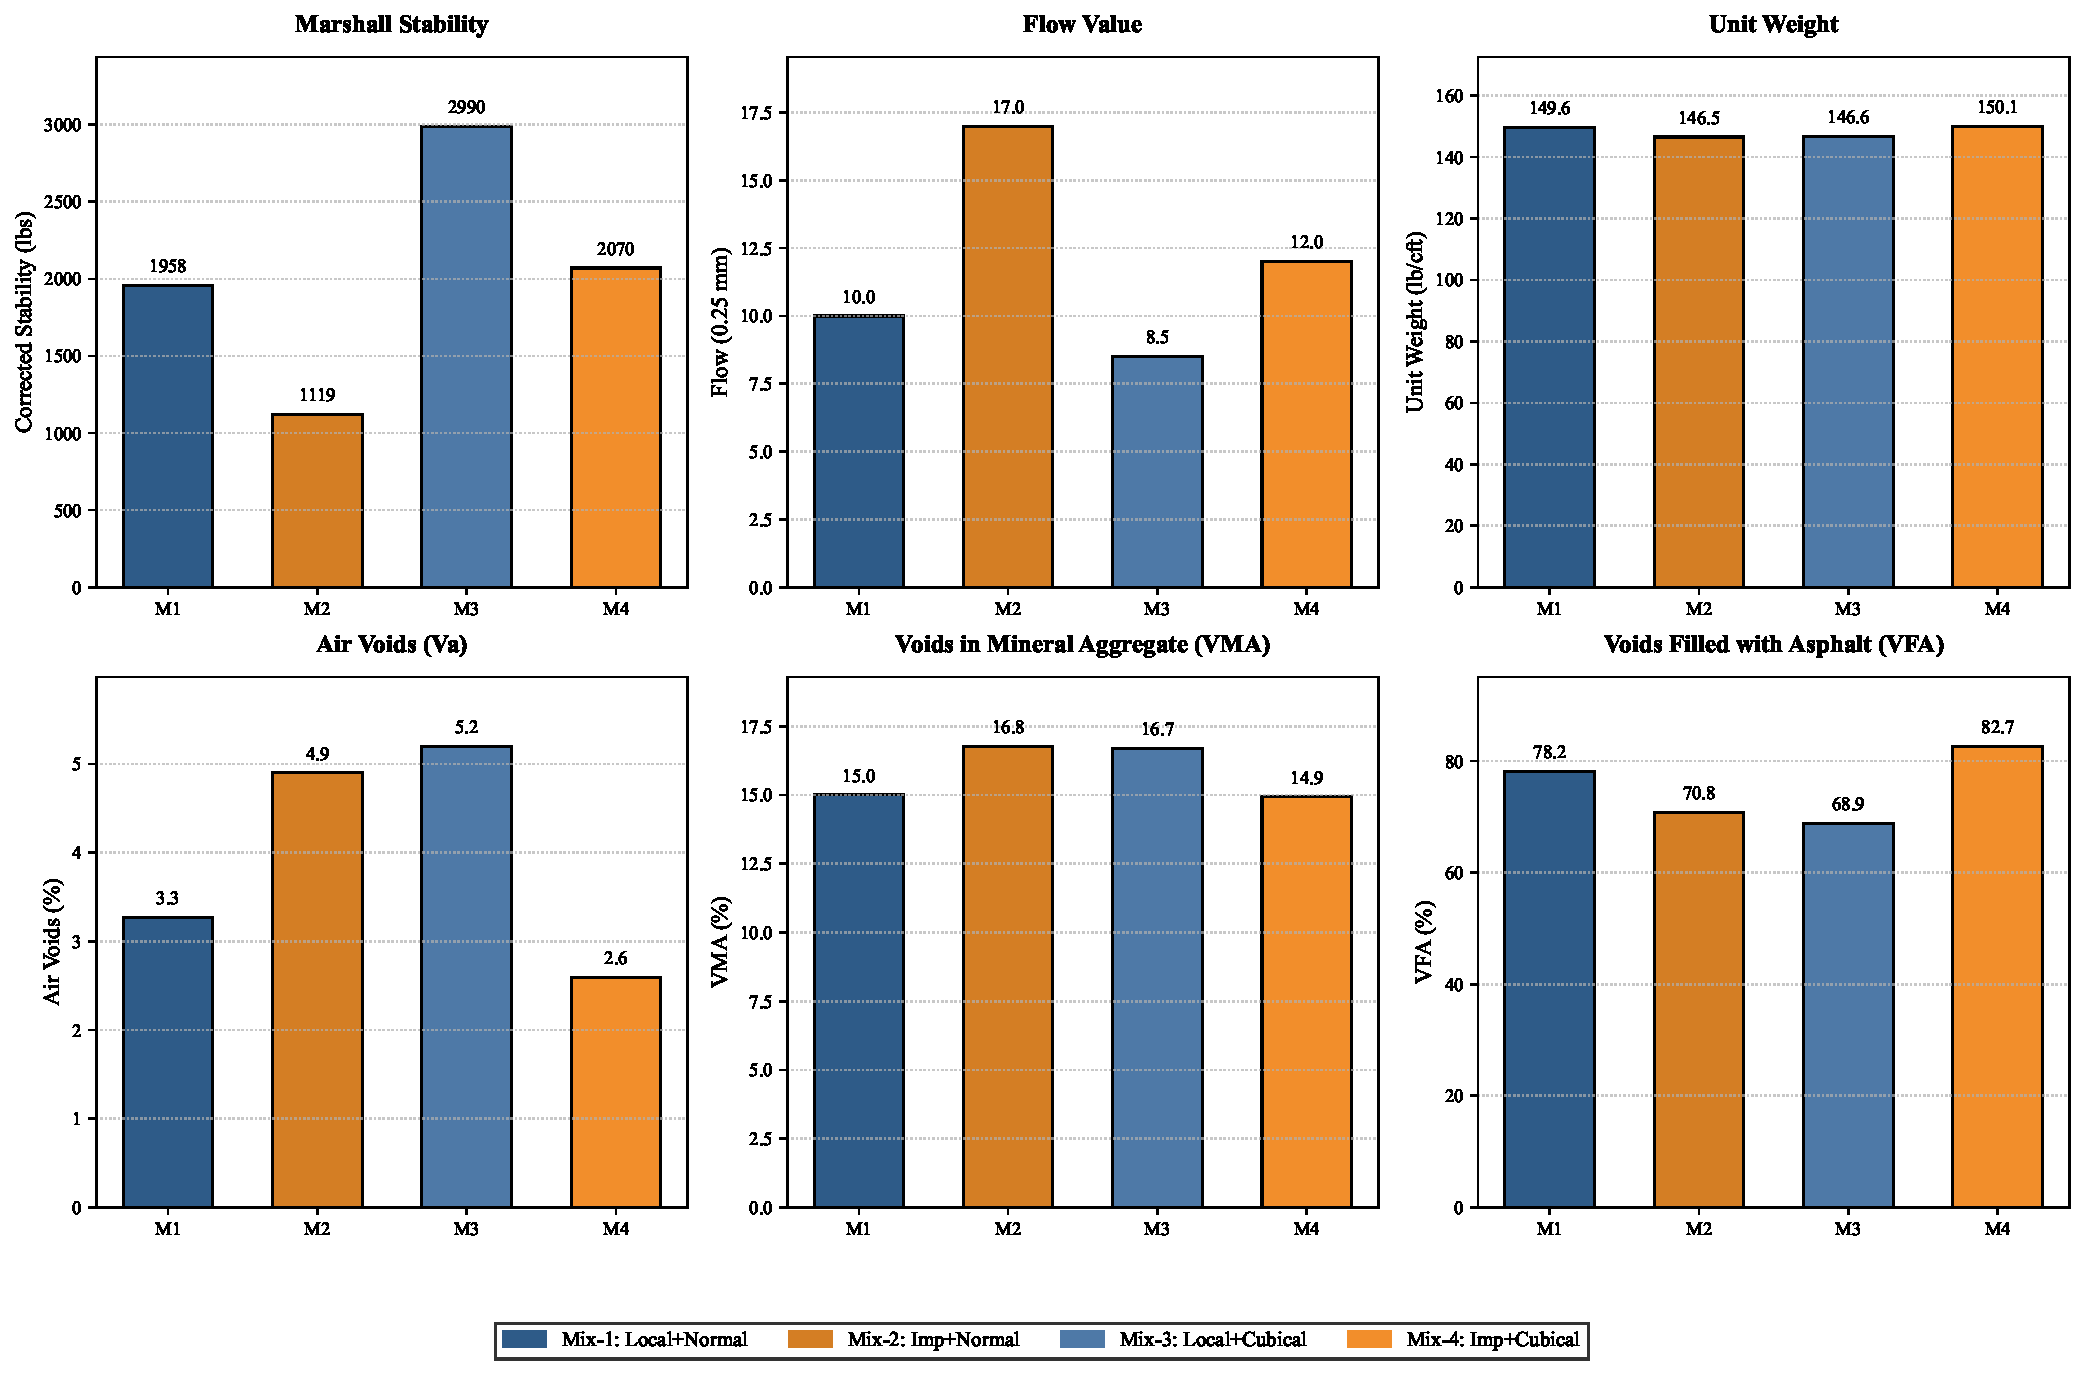
\includegraphics[width=\textwidth]{graphics/performance_assessment.pdf}
    \caption{Performance assessment of the four bituminous mix variants across Marshall stability, flow, and volumetric parameters.}
    \label{fig:performance_assessment}
\end{figure}

\textbf{B. Load Bearing Capacity (Marshall Stability):}
The left subplot of Figure~\ref{fig:mix_comparison} shows that adding 20\% cubical aggregates raised the load-bearing capacity for both binder types. The mix with local ERL bitumen and 20\% cubical aggregates gave the highest Marshall stability (2991 lbs). The ERL bitumen has a lower penetration value, which makes the mix stiffer. Bagampadde et al. (2006) \cite{bagampadde2006impact} reported something similar: bitumen with lower penetration grades tends to produce stronger mixes. At the other end, the imported bitumen with normal aggregates gave the lowest stability of all four mixes (1119 lbs).

\textbf{C. Deformation (Flow Value):}
The right subplot of Figure~\ref{fig:mix_comparison} shows the flow values, measured in units of 0.25\,mm. The imported bitumen with normal aggregates had the highest flow (17 units), which means this mix is the most prone to permanent deformation and rutting. The local bitumen with 20\% cubical aggregates had a flow of just 8.5 units, well within the RHD limits for heavy-duty pavements.

\textbf{D. Required Pavement Thickness:}
Under the AASHTO structural design guidelines for flexible pavements, the structural layer coefficient ($a_1$) of the bituminous surfacing depends on its Marshall stability and resilient modulus. Since the local bitumen with 20\% cubical aggregates mix had the highest stability, it has the highest $a_1$ value. In practical terms, this means that to reach a given target Structural Number (SN) for a particular traffic load, this mix would need a thinner asphalt layer than any of the other three variants. The imported bitumen with normal aggregates, having the lowest structural coefficient, would need the thickest layer.

\textbf{E. Cost Effectiveness:}
Pavement thickness has a direct effect on construction costs. Because the local bitumen and 20\% cubical aggregates mix can reach the needed structural capacity with a thinner layer, it cuts down the total volume of bituminous material needed per kilometre of road. The savings on materials can offset whatever extra costs come from local refining or sorting aggregates by shape, making this mix a cost-effective option over the pavement's service life.

\begin{figure}[H]
    \centering
    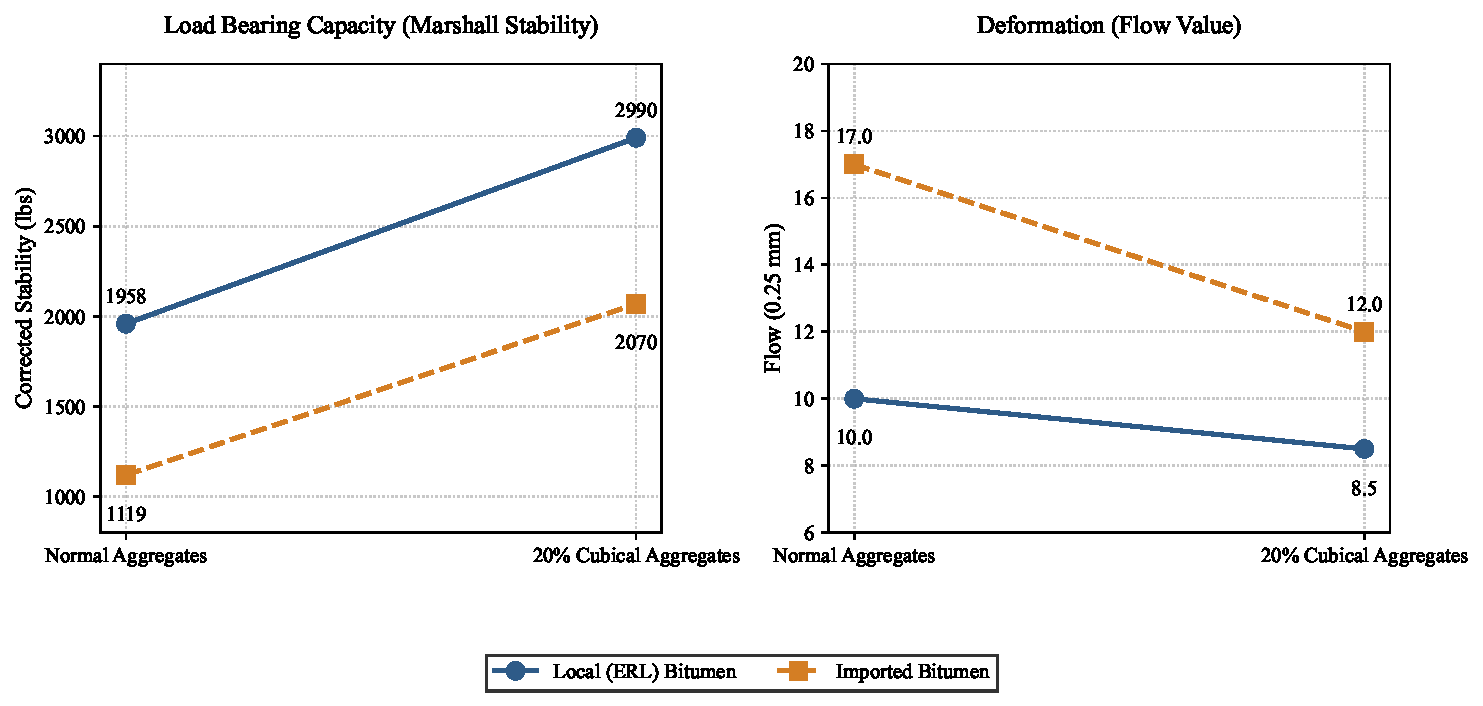
\includegraphics[width=\textwidth]{graphics/mix_comparison.pdf}
    \caption{Interaction line plots comparing Marshall stability and flow across four bituminous mix variants.}
    \label{fig:mix_comparison}
\end{figure}

\subsection{Proposed Roadmap for Cost-Effective Road Construction in Bangladesh}

Road construction in Bangladesh is expensive partly because of weak subgrade soils, heavy monsoon rains, and dependence on imported materials. Drawing on our findings and the existing literature, we propose a two-level strategy that could improve pavement durability while keeping costs manageable.

The idea is to combine subgrade improvement with a better surface mix:

\begin{enumerate}
    \item \textbf{Foundation Level (Subgrade Stabilization):} The subgrade carries the load of the entire pavement structure. In Bangladesh, the subgrade is often weak, which means the base and sub-base layers have to be built thicker to compensate. Sood and Bansal \cite{sood2015evaluation} showed that treating weak subgrade soils with lime and fly ash raises the CBR. A stronger subgrade means the layers above it can be thinner.
    \item \textbf{Surface Level (Optimized Bituminous Mix):} On top of the stabilized foundation, the surface course needs to resist rutting and moisture damage. Our experimental results showed that combining local ERL bitumen with 20\% cubical aggregates gave a Marshall stability of 2991 lbs and a flow of 8.5 units. In terms of pavement design (for example, using the AASHTO 1993 method), this high stability translates to a higher structural layer coefficient ($a_1$).
\end{enumerate}

\textbf{Techno-Economic Summary:}
If the foundation is strengthened with lime and fly ash and the surface course uses ERL bitumen with 20\% cubical aggregates, the required structural number (SN) can be reached with thinner pavement layers. Using less aggregate and less bitumen per kilometre of road is a practical way to lower construction costs in Bangladesh without compromising the structural performance of the pavement.

\section{Conclusion}

\subsection{Summary of Findings}
This study compared locally produced Eastern Refinery bitumen with imported bitumen in a laboratory setting, looking specifically at how aggregate particle shape (20\% cubical replacement) affects the Marshall mix design properties. From the experiments and volumetric analyses, the main findings are:
\begin{itemize}
    \item The locally refined ERL bitumen had better rheological properties than the imported binder, including higher viscosity and more consistent penetration grades. It met or exceeded the test requirements across the board.
    \item Replacing 20\% of the coarse aggregate with cubical particles and using local ERL bitumen (Mix-3) gave a Marshall stability of 2991 lbs (13.3 kN) and a flow of 8.5 units.
    \item The volumetric analysis showed that while the conventional mixes stayed within standard tolerances, the imported bitumen with 20\% cubical aggregates (Mix-4) produced air voids of only 2.59\% and a VFA of 82.65\%, which increases the risk of binder bleeding under traffic.
    \item Local ERL bitumen paired with cubical aggregates gives a mix that is both structurally strong and volumetrically stable, meaning higher load-bearing capacity without compromising durability.
    \item \textbf{Proposed Roadmap for Bangladesh:} A two-level strategy is proposed: (1) \textit{Foundation Level:} stabilize weak subgrade soils with lime and fly ash to raise the CBR; and (2) \textit{Surface Level:} use local ERL bitumen with at least 20\% cubical aggregates. Together, these steps would reduce the volume of imported materials needed.
\end{itemize}

\subsection{Recommendations for Practice}
From the experimental results, we recommend a two-level approach for road infrastructure in Bangladesh:

\begin{enumerate}
    \item \textbf{Foundation Level (Subgrade Stabilization):} For areas with weak subgrade soils, treating the soil with lime or fly ash is recommended. This raises the California Bearing Ratio (CBR) and allows the pavement layers above to be thinner.
    \item \textbf{Surface Level (Optimized Bituminous Mix):} The Roads and Highways Department (RHD) should consider adding quality control requirements for imported bitumen and introducing aggregate shape sorting into the specifications. Setting a minimum threshold of $20\%$ cubical coarse aggregates, to be used with local ERL bitumen, would improve the interlocking matrix of the mix.
\end{enumerate}

Making these changes would raise the structural layer coefficient ($a_1$) of the surfacing course, which means the same structural performance can be achieved with less material. Over time, this reduces lifecycle costs for highway projects.

\subsection{Future Work}
Several areas remain open for further investigation:
\begin{itemize}
    \item \textbf{Indirect Tensile Strength (ITS) Testing:} Running ITS tests (ASTM D6931) would help evaluate how the different mix combinations resist tensile loading and fracture.
    \item \textbf{Moisture Susceptibility and Climate Resistance:} Retained stability tests (Marshall immersion) or Tensile Strength Ratio (TSR) tests would show how well these mixes resist stripping under conditions similar to Bangladesh's monsoon climate.
    \item \textbf{Rutting and Fatigue Evaluation:} The Hamburg Wheel Tracking Test (AASHTO T 324) could be used to measure rutting depth, and the Four-Point Bending Beam Fatigue Test (AASHTO T 321) would give information on cracking resistance under repeated loading.
    \item \textbf{Evaluation of Polymer Modified Bitumen (PMB):} It would be worth investigating what happens when 5\% SBS (Styrene-Butadiene-Styrene) polymer is added to these base bitumens to produce PMB, following LGED specifications. Such a study could show how much polymer modification improves load-bearing capacity and fatigue life.
    \item \textbf{Performance Enhancement of Imported Bitumen:} Since Bangladesh will likely continue importing bitumen, future work should look into ways to improve imported binders. Additives like 5\% SBS polymer, crumb rubber, or waste plastics could potentially bring the structural and rheological properties of imported bitumen closer to those of the local product.
\end{itemize}

\clearpage
\phantomsection
\renewcommand{\refname}{\centering\normalfont\Large\bfseries REFERENCES}
\addcontentsline{toc}{section}{REFERENCES}
\begin{singlespace}
\let\oldbibliography\thebibliography
\renewcommand{\thebibliography}[1]{%
  \oldbibliography{#1}%
  \setlength{\itemsep}{14pt}%
  \setlength{\parskip}{0pt}%
}
\bibliographystyle{plain}
\bibliography{biblography}
\end{singlespace}

\clearpage
\phantomsection
\addcontentsline{toc}{section}{APPENDIX}
\begin{center}
    \textbf{\Large APPENDIX}
\end{center}
\vspace{1.5cm}

\begin{center}
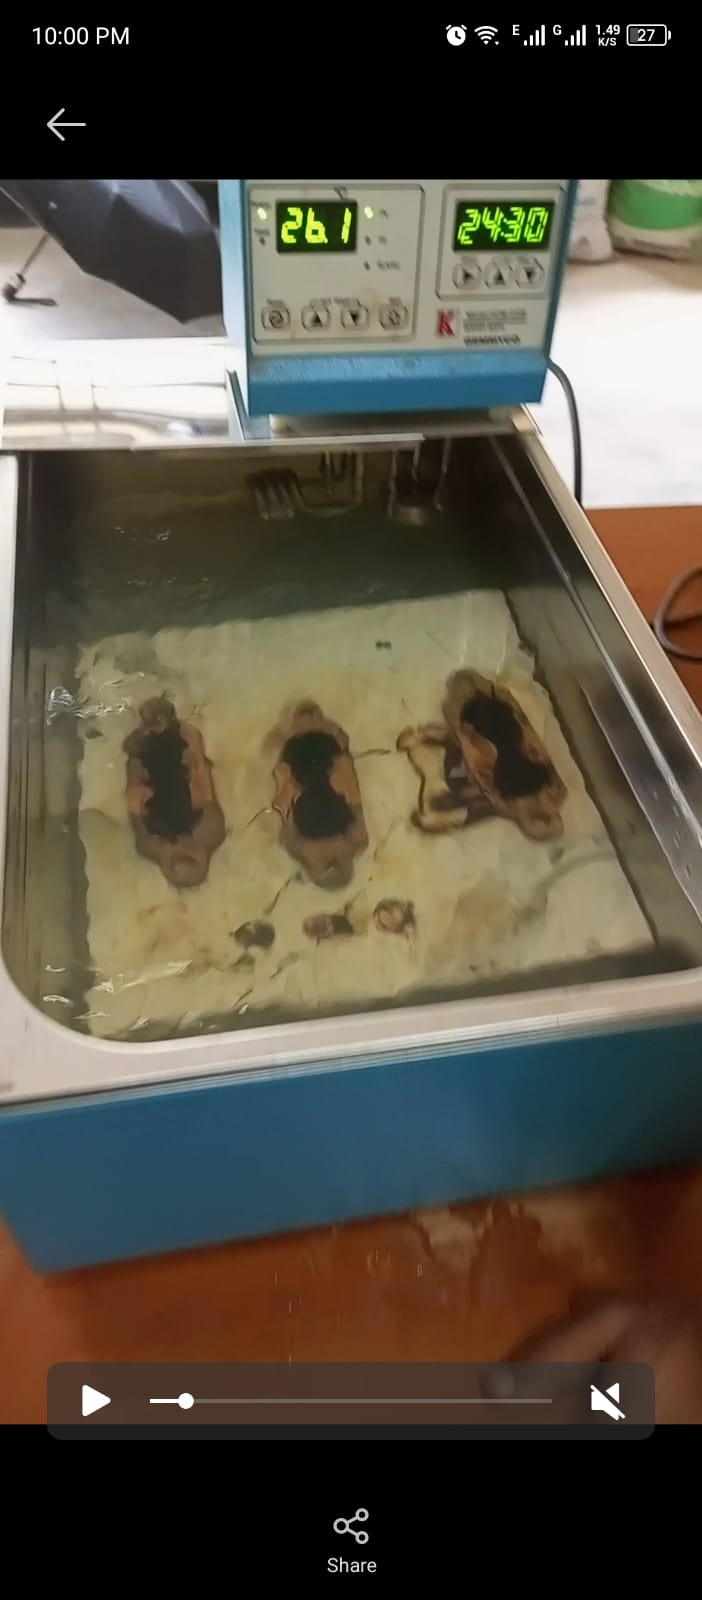
\includegraphics[width=4in, height=4in]{albums/appendix_01.jpeg}
\vspace{0.5cm}

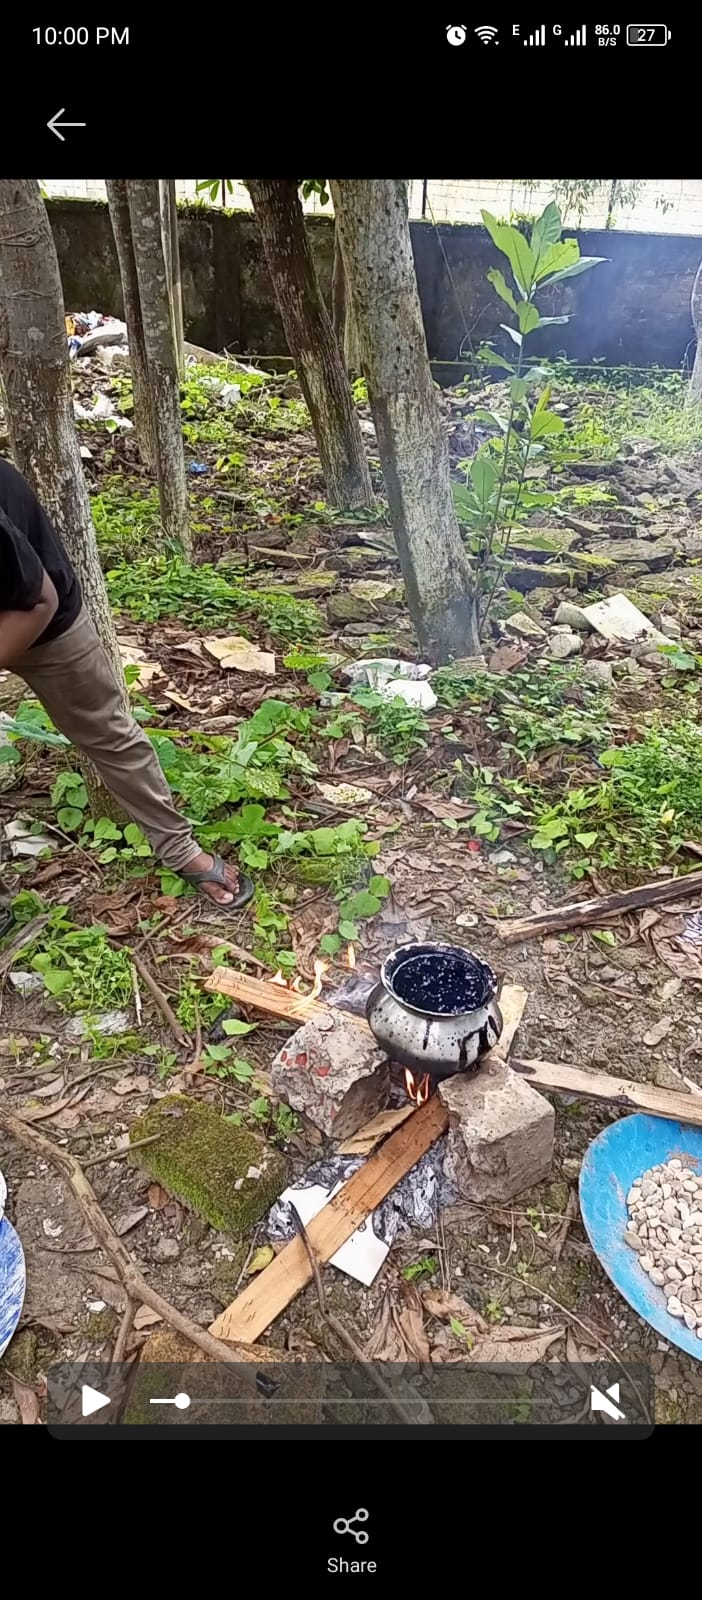
\includegraphics[width=4in, height=4in]{albums/appendix_02.jpeg}
\vspace{0.5cm}

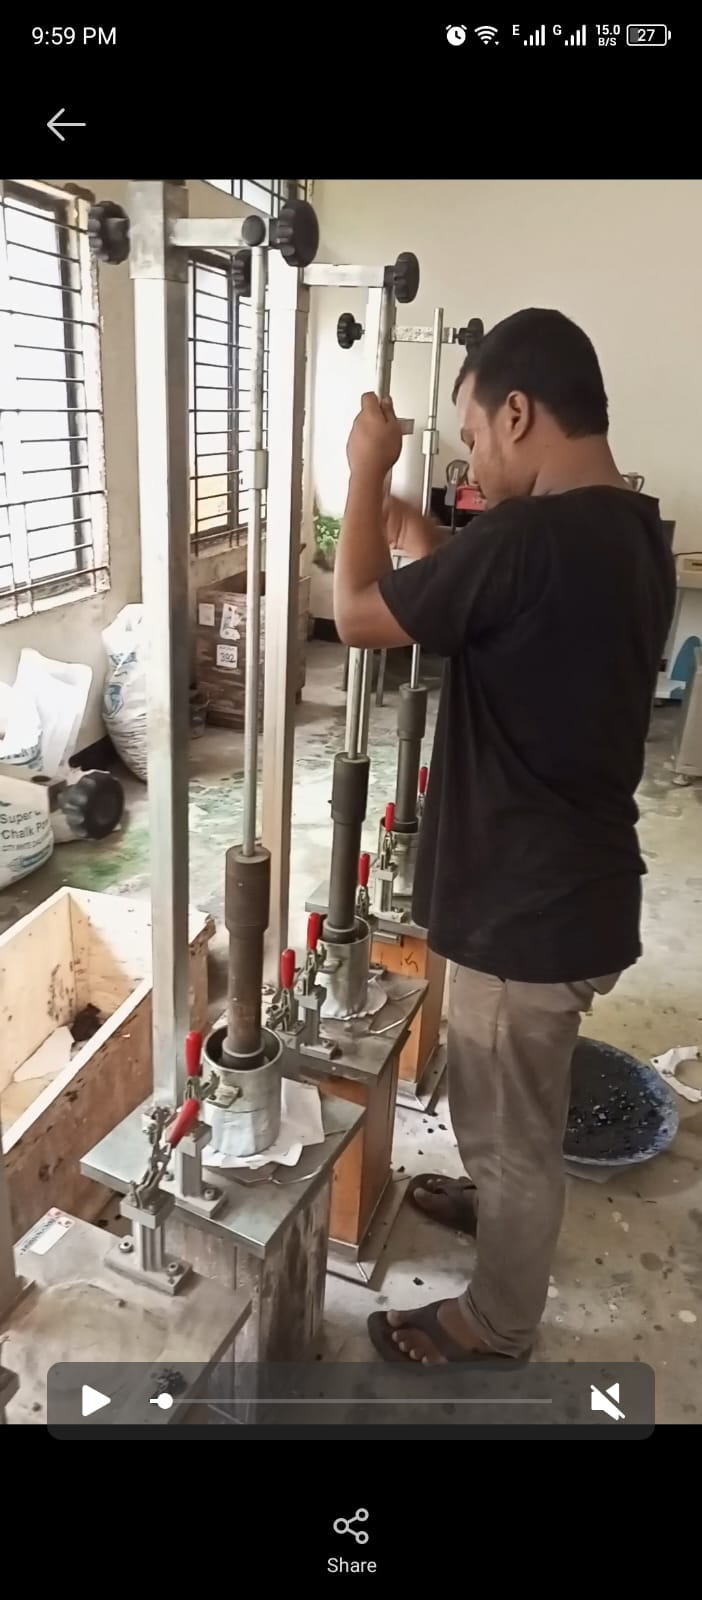
\includegraphics[width=4in, height=4in]{albums/appendix_03.jpeg}
\vspace{0.5cm}

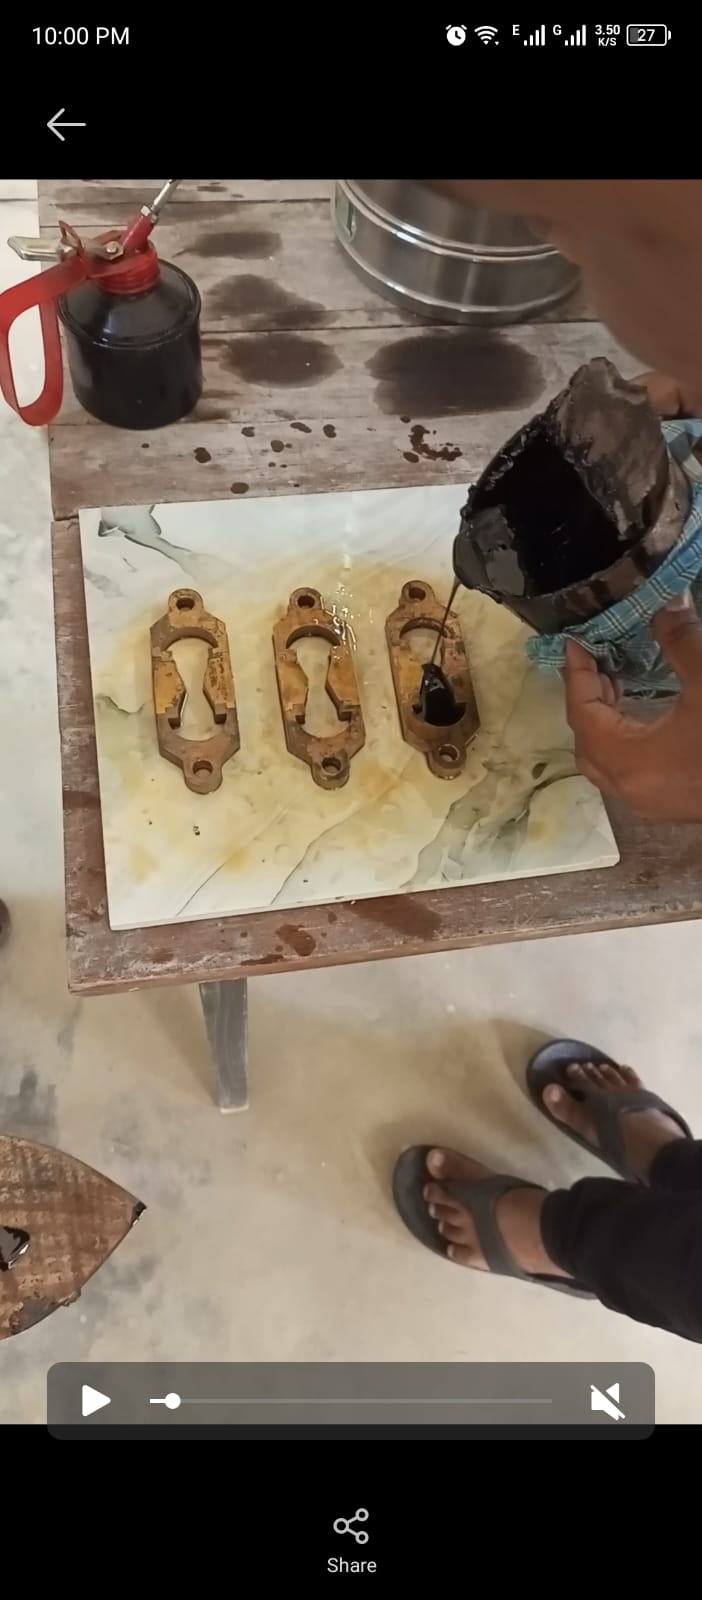
\includegraphics[width=4in, height=4in]{albums/appendix_04.jpeg}
\vspace{0.5cm}

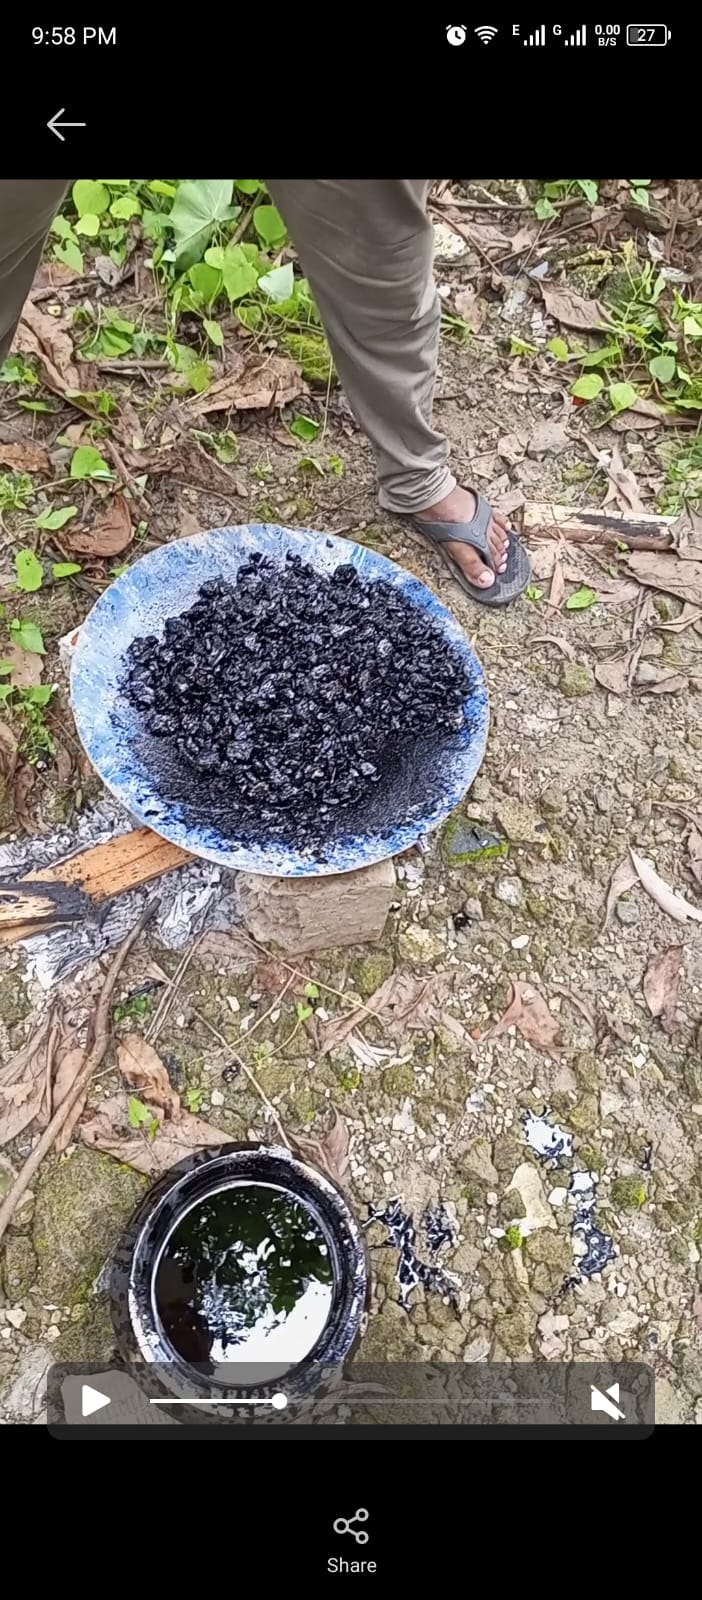
\includegraphics[width=4in, height=4in]{albums/appendix_05.jpeg}
\vspace{0.5cm}

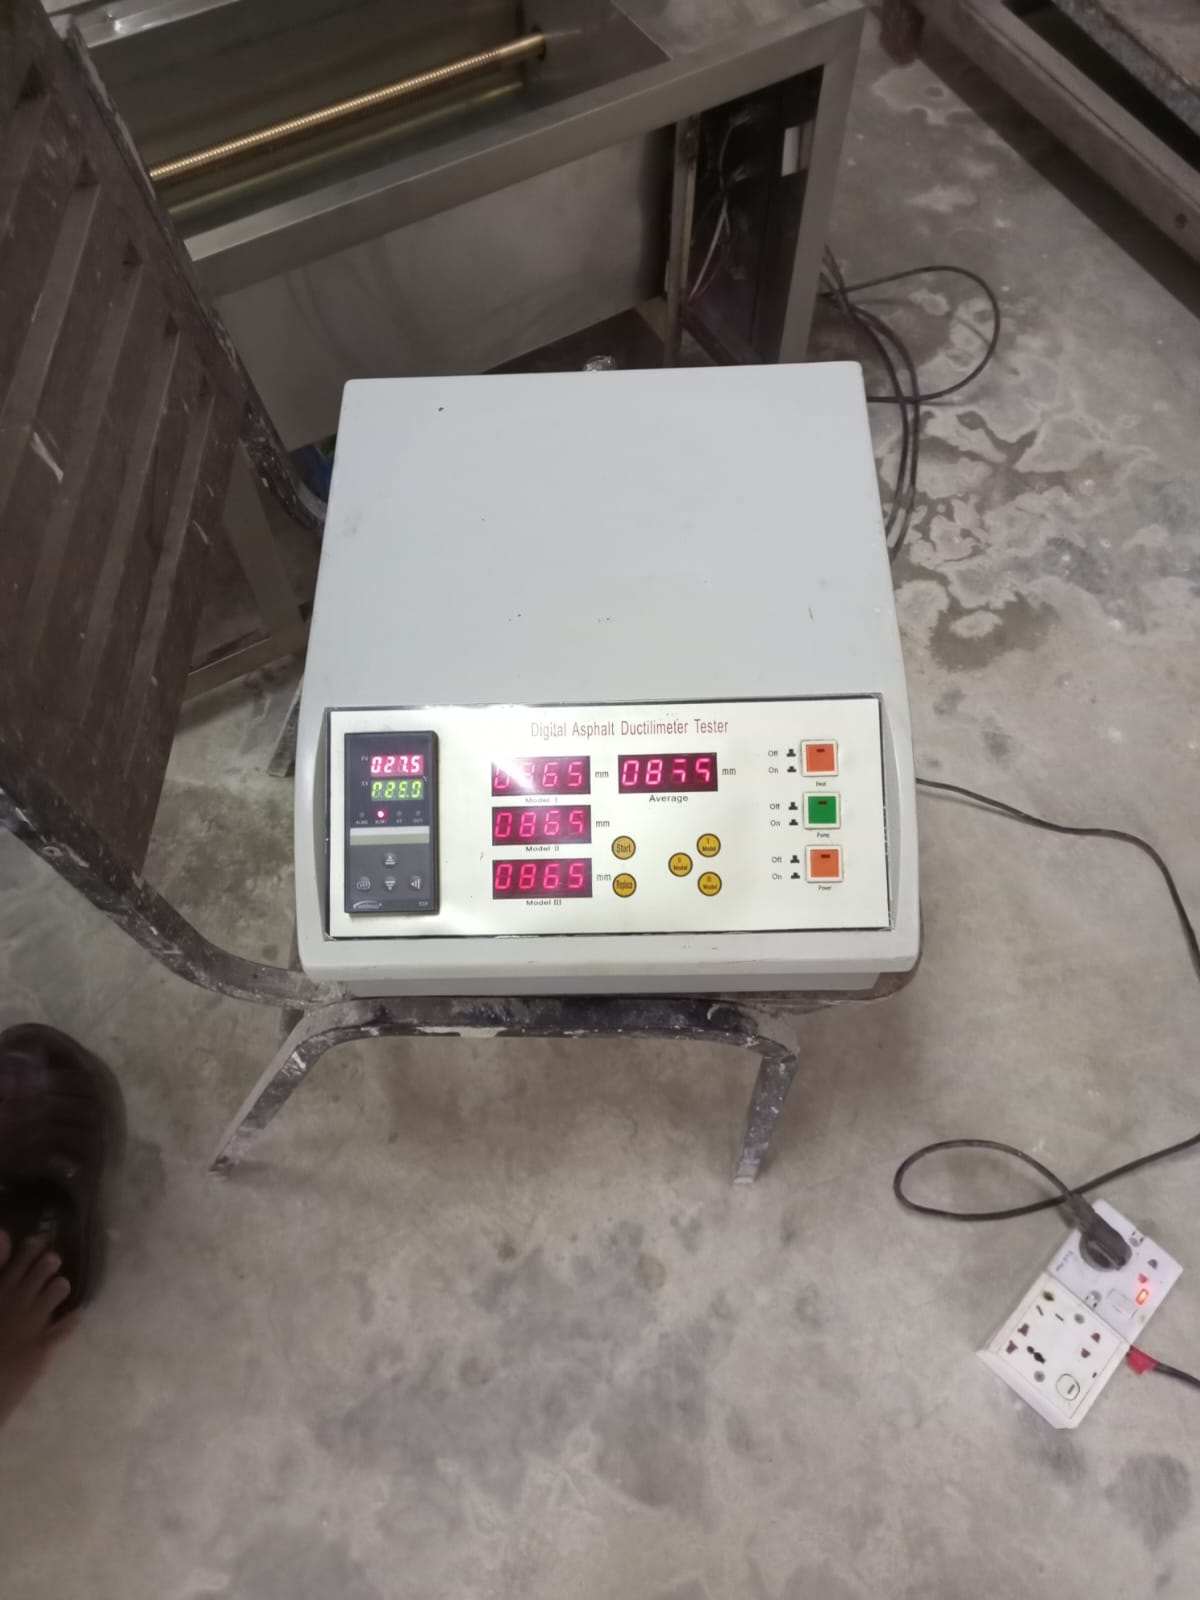
\includegraphics[width=4in, height=4in]{albums/appendix_06.jpeg}
\vspace{0.5cm}

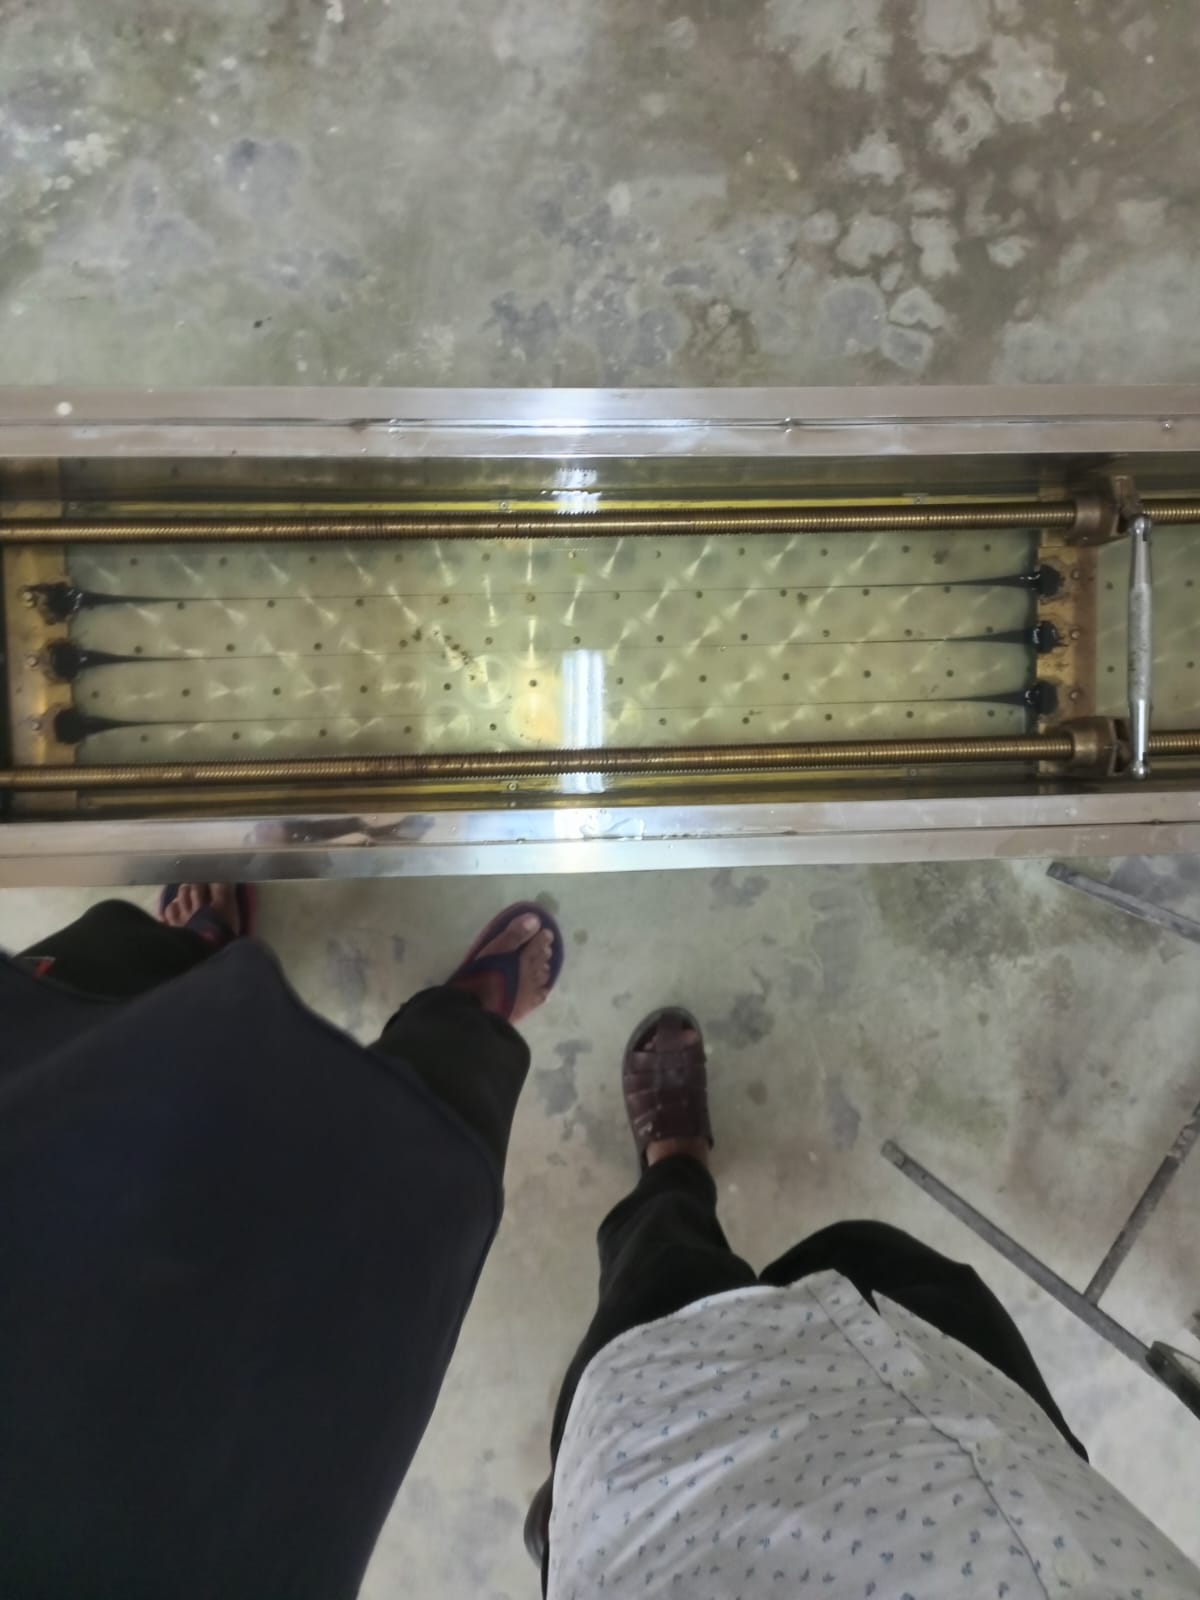
\includegraphics[width=4in, height=4in]{albums/appendix_07.jpeg}
\vspace{0.5cm}

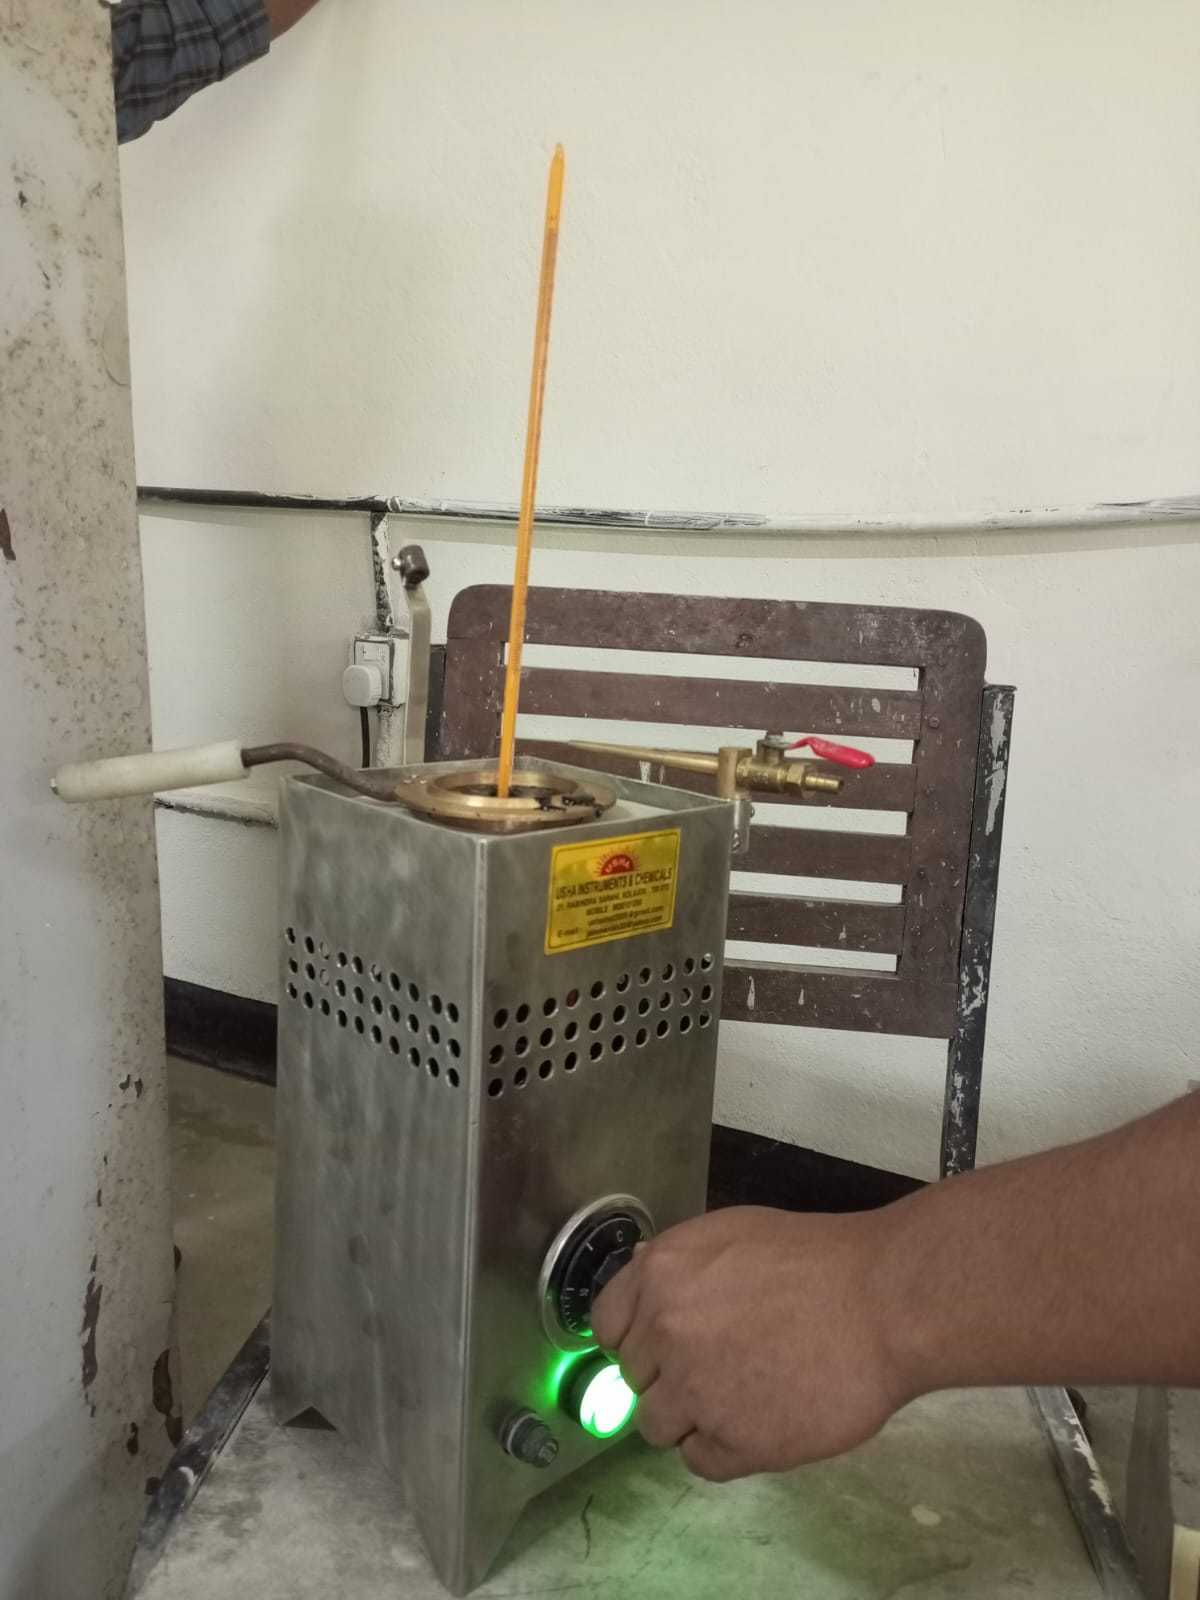
\includegraphics[width=4in, height=4in]{albums/appendix_08.jpeg}
\vspace{0.5cm}

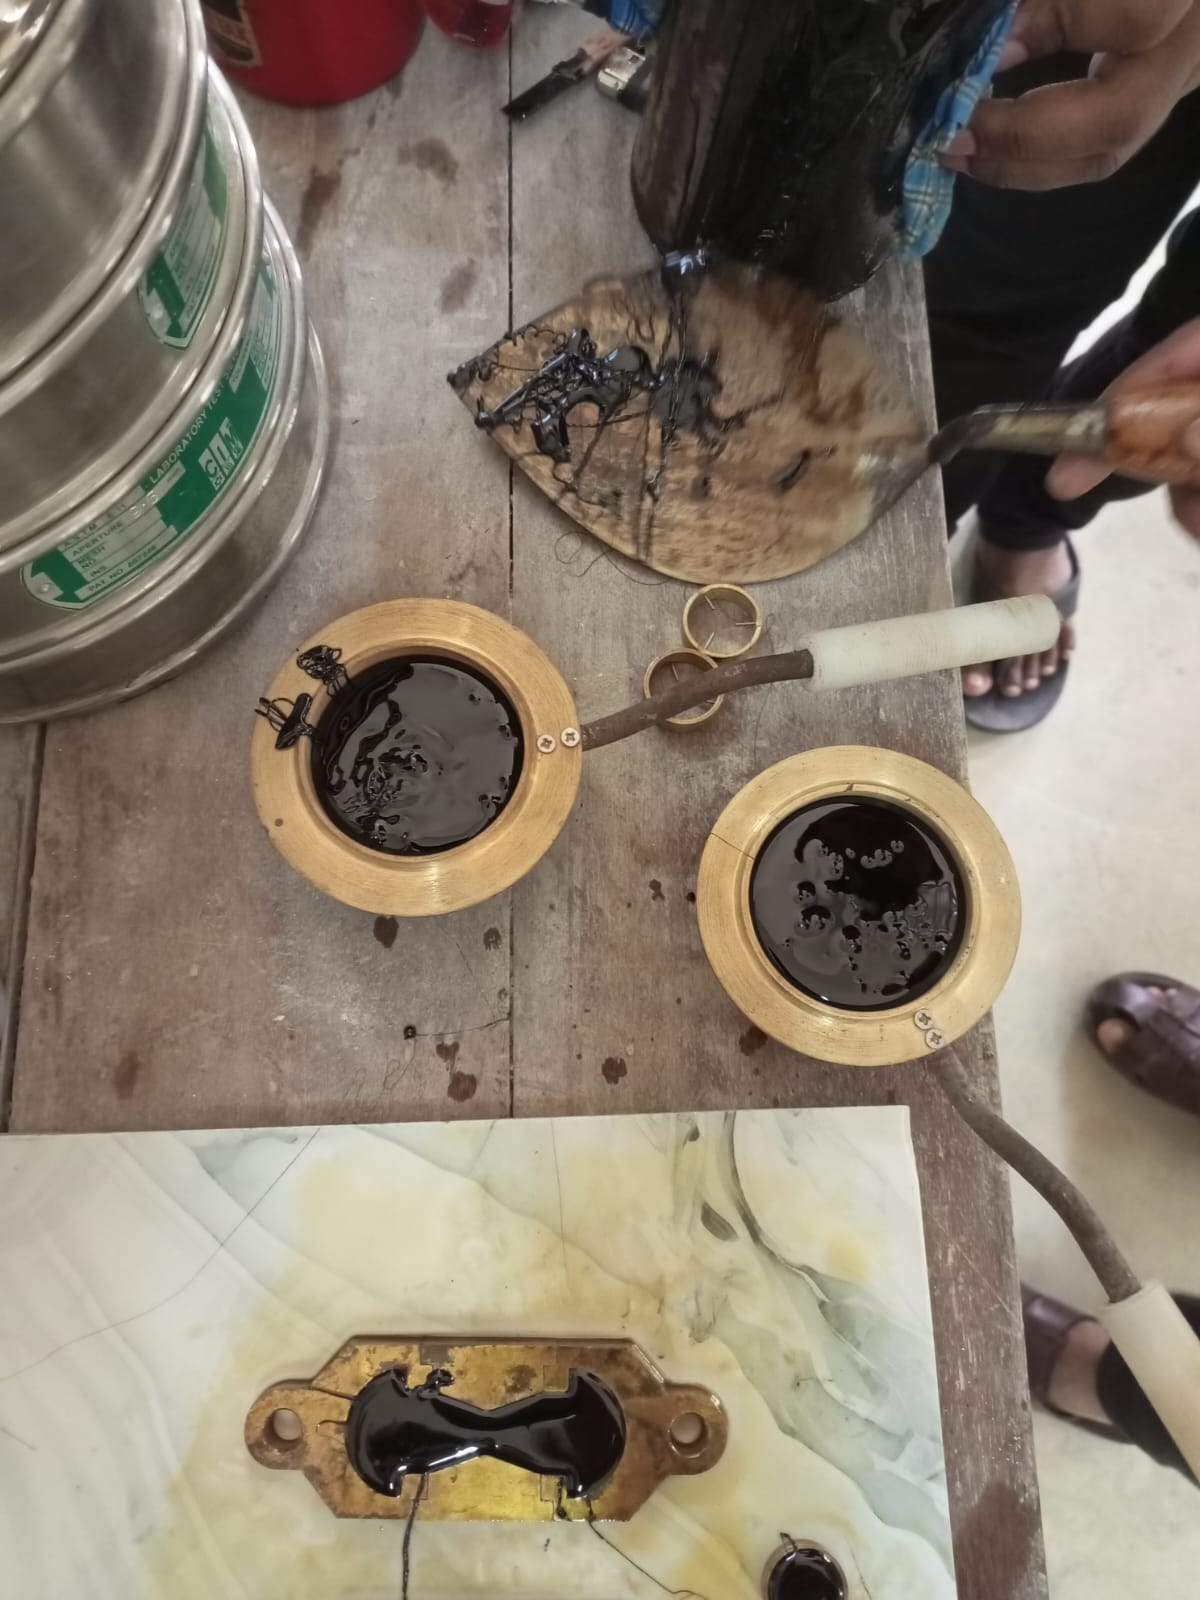
\includegraphics[width=4in, height=4in]{albums/appendix_09.jpeg}
\vspace{0.5cm}

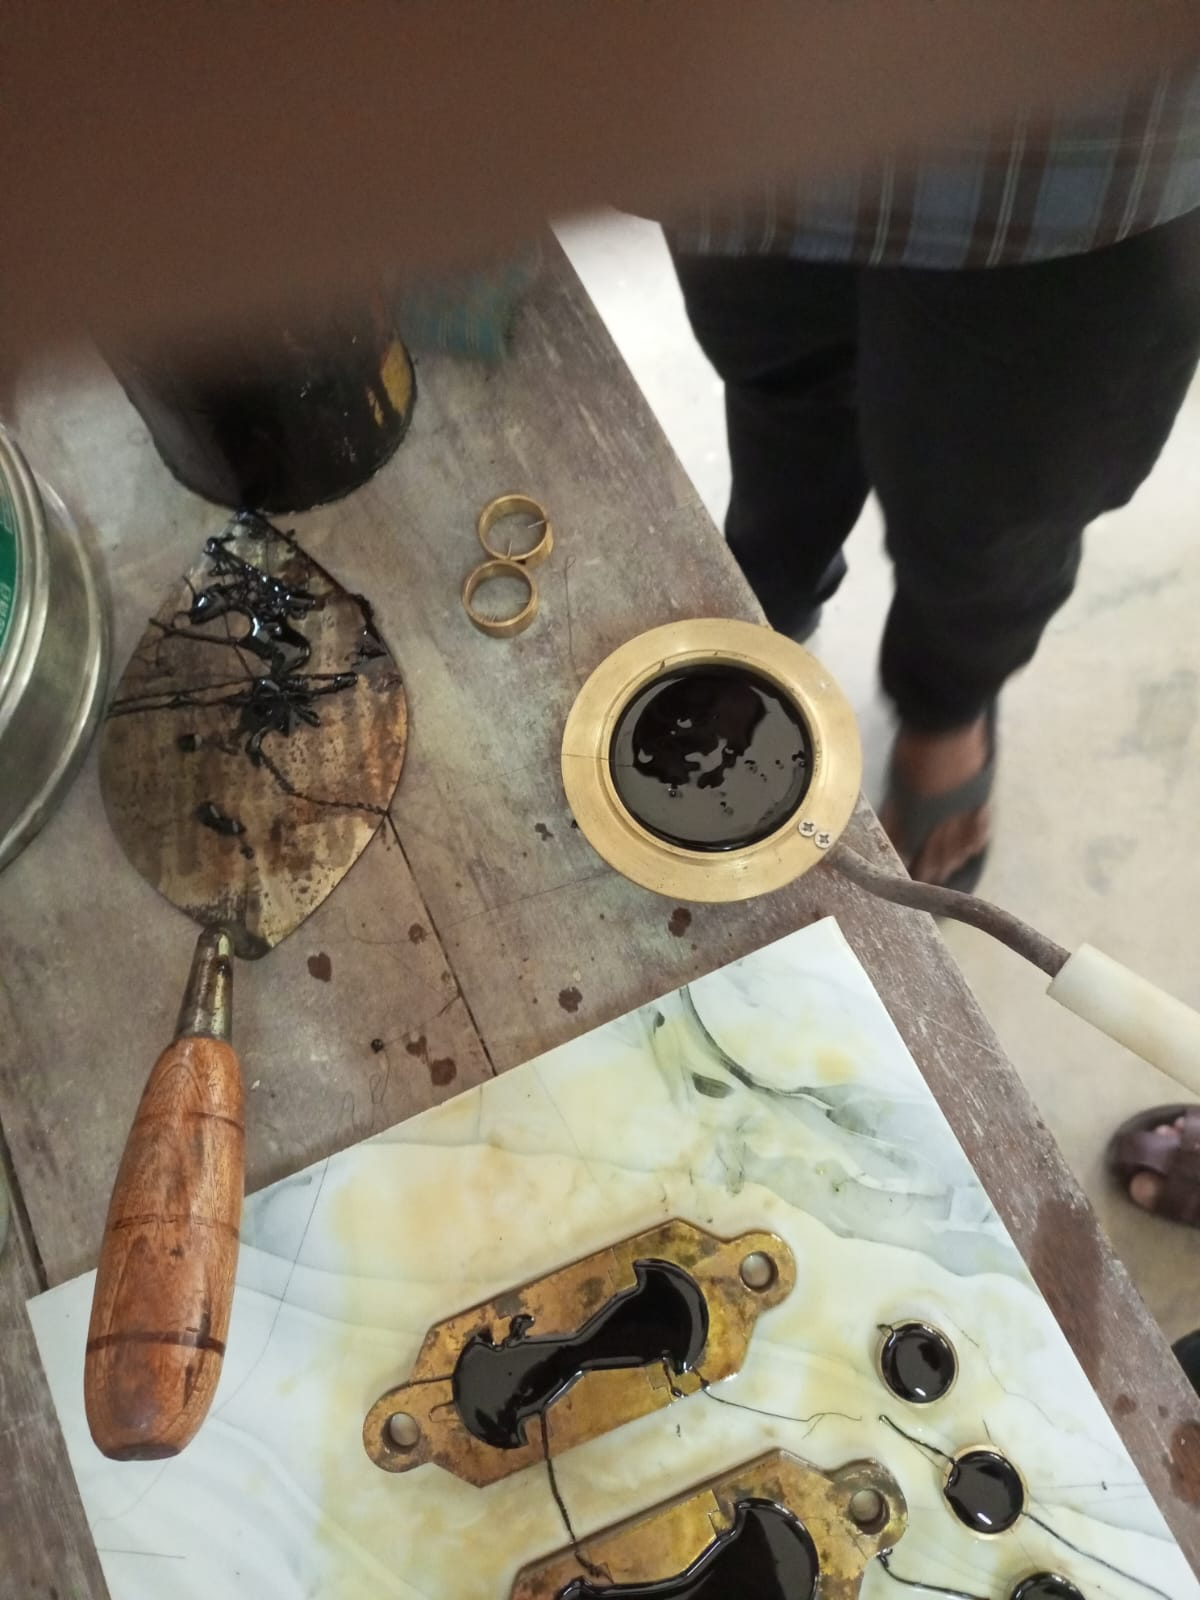
\includegraphics[width=4in, height=4in]{albums/appendix_10.jpeg}
\vspace{0.5cm}

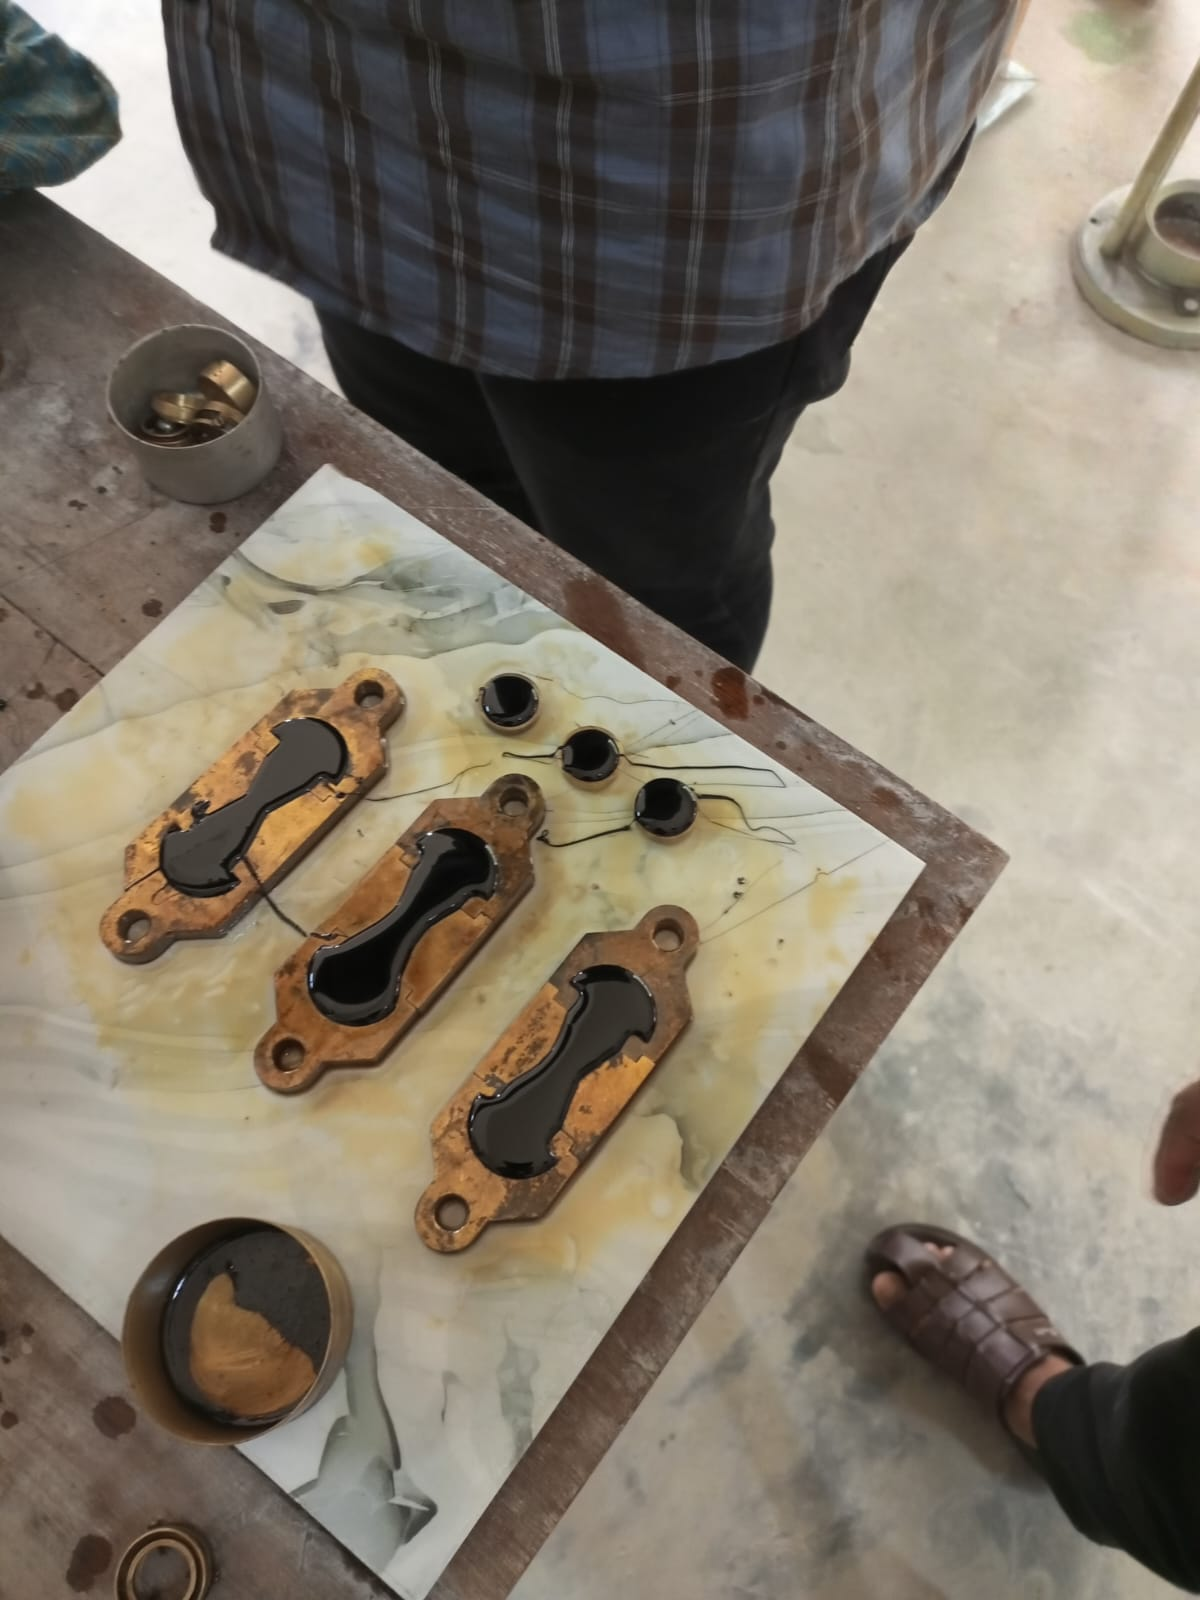
\includegraphics[width=4in, height=4in]{albums/appendix_11.jpeg}
\vspace{0.5cm}

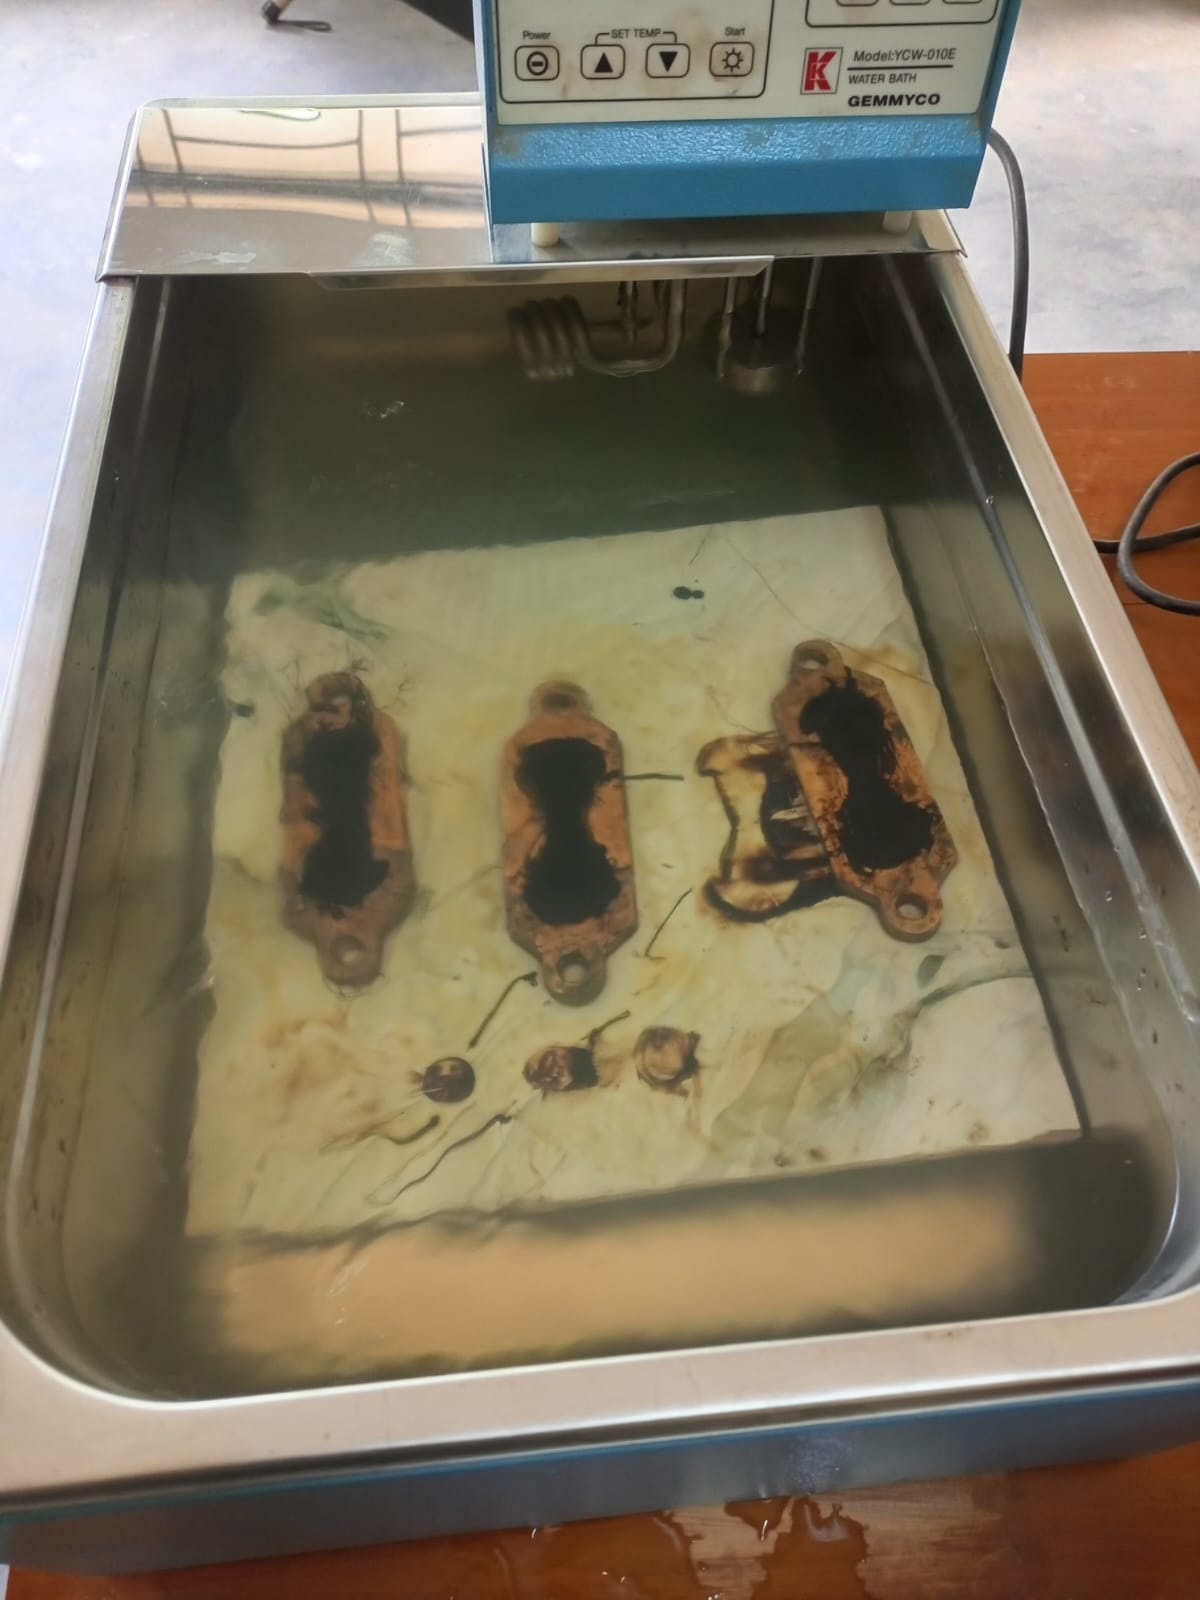
\includegraphics[width=4in, height=4in]{albums/appendix_12.jpeg}
\vspace{0.5cm}

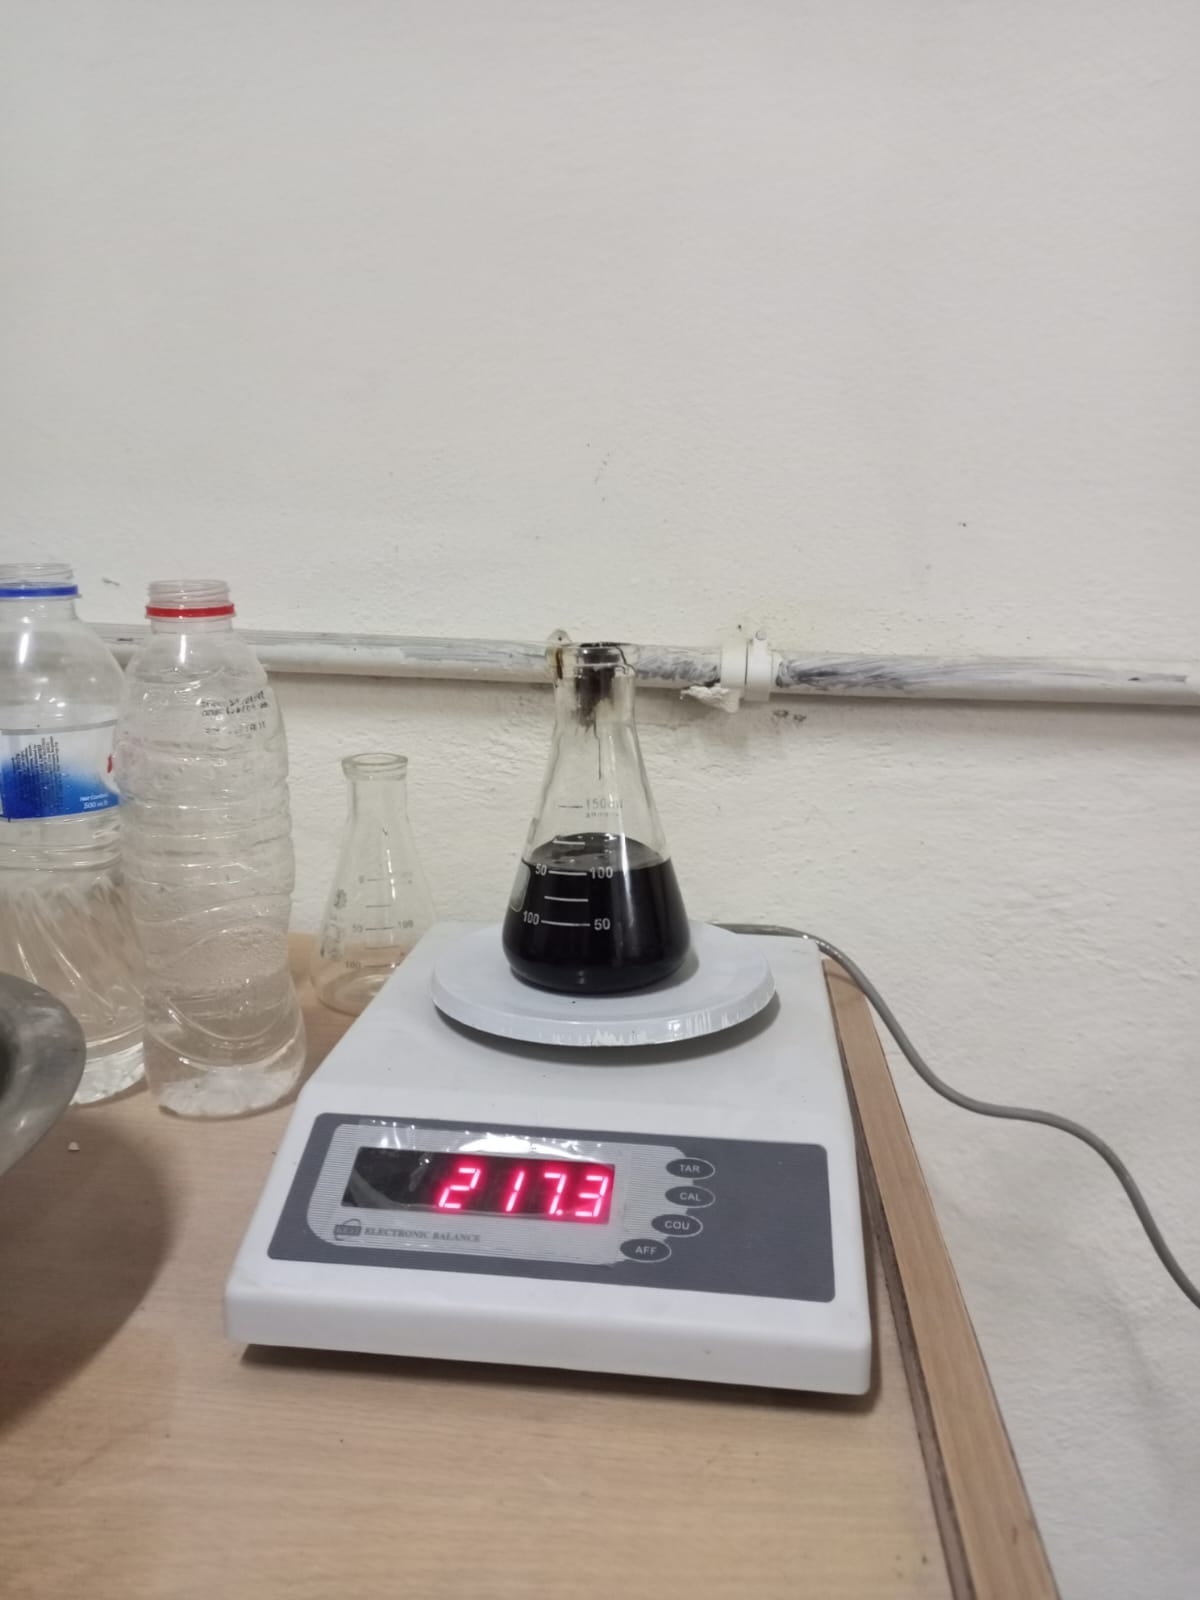
\includegraphics[width=4in, height=4in]{albums/appendix_13.jpeg}
\vspace{0.5cm}

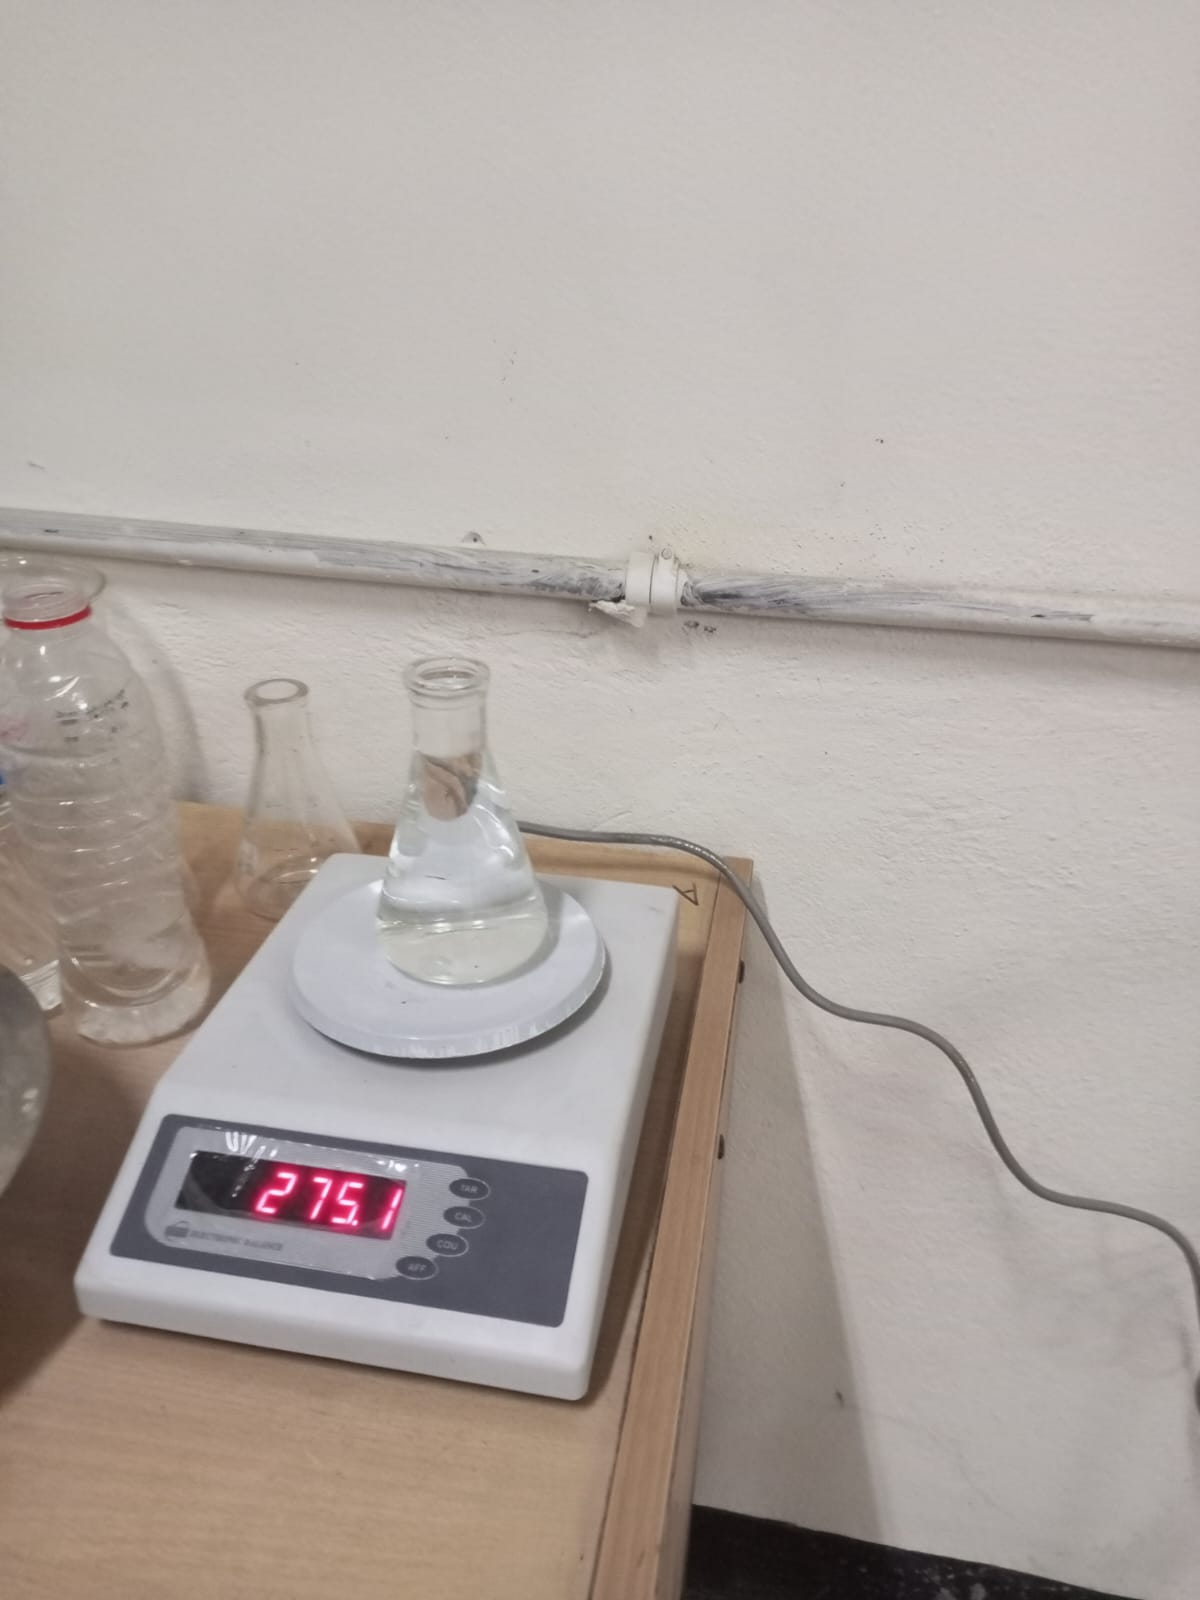
\includegraphics[width=4in, height=4in]{albums/appendix_14.jpeg}
\vspace{0.5cm}

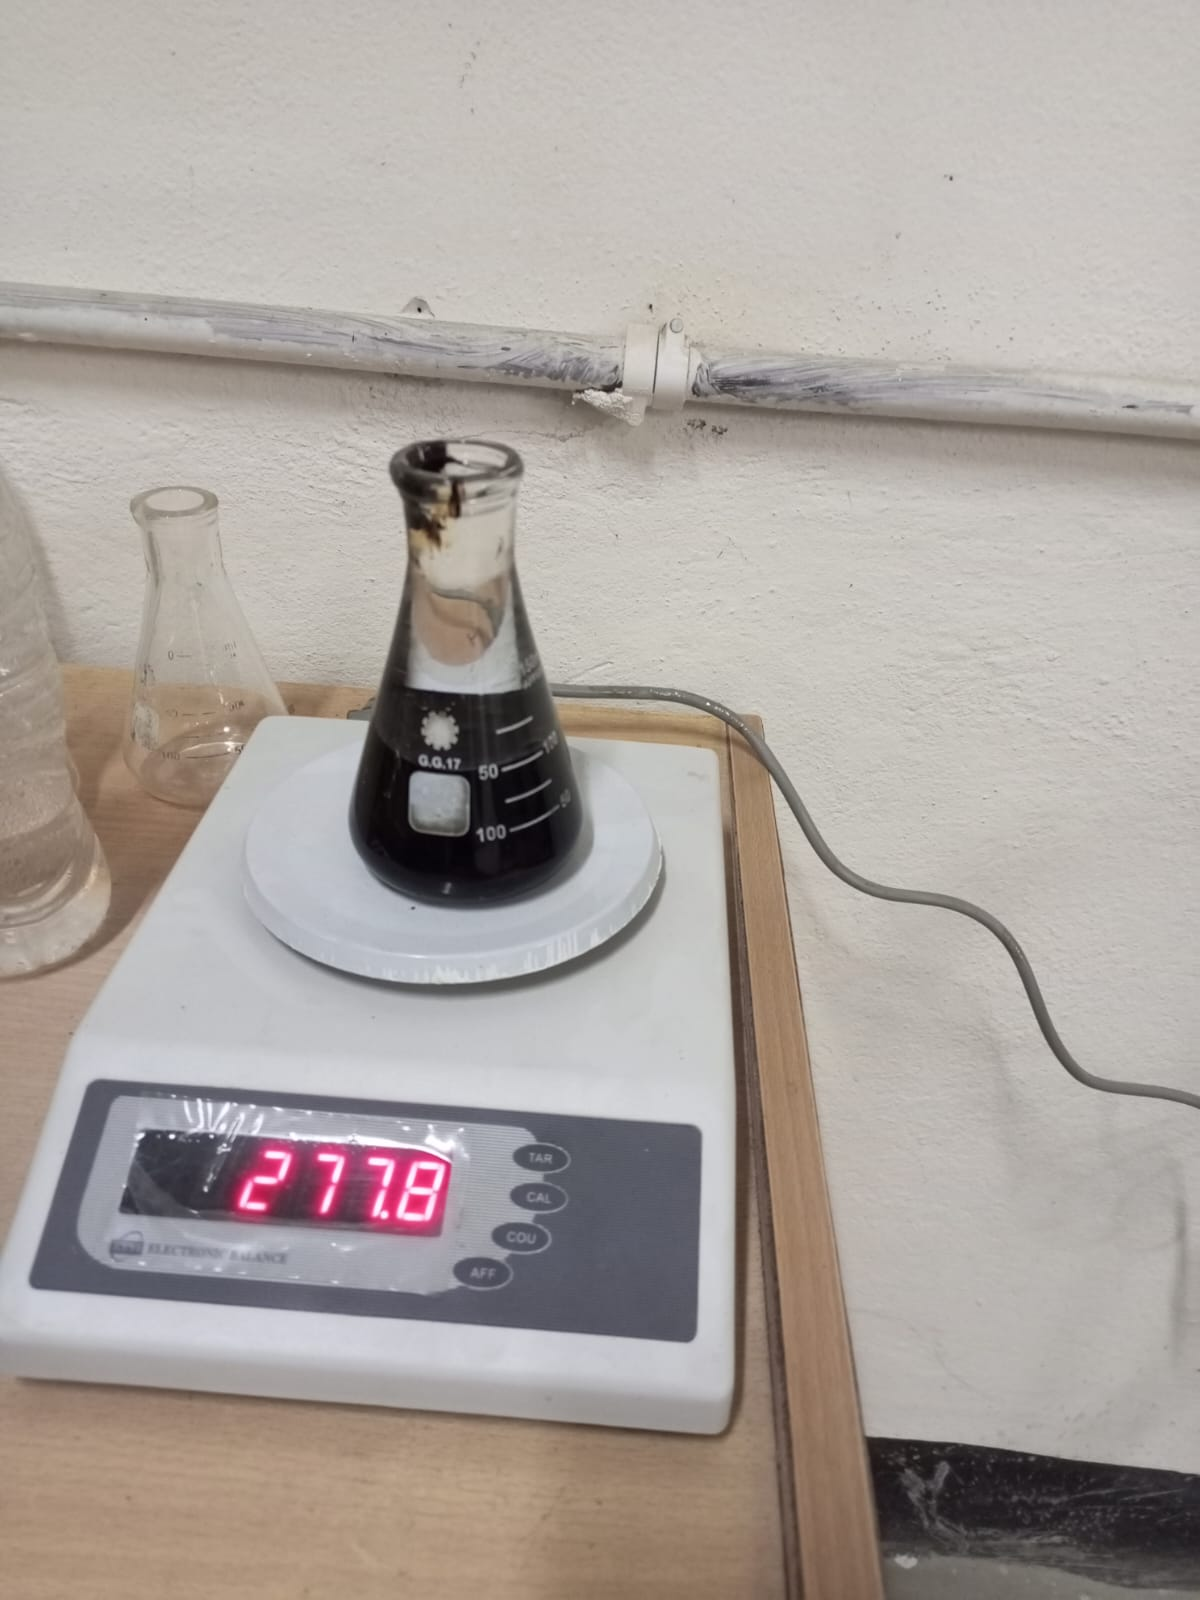
\includegraphics[width=4in, height=4in]{albums/appendix_15.jpeg}
\vspace{0.5cm}

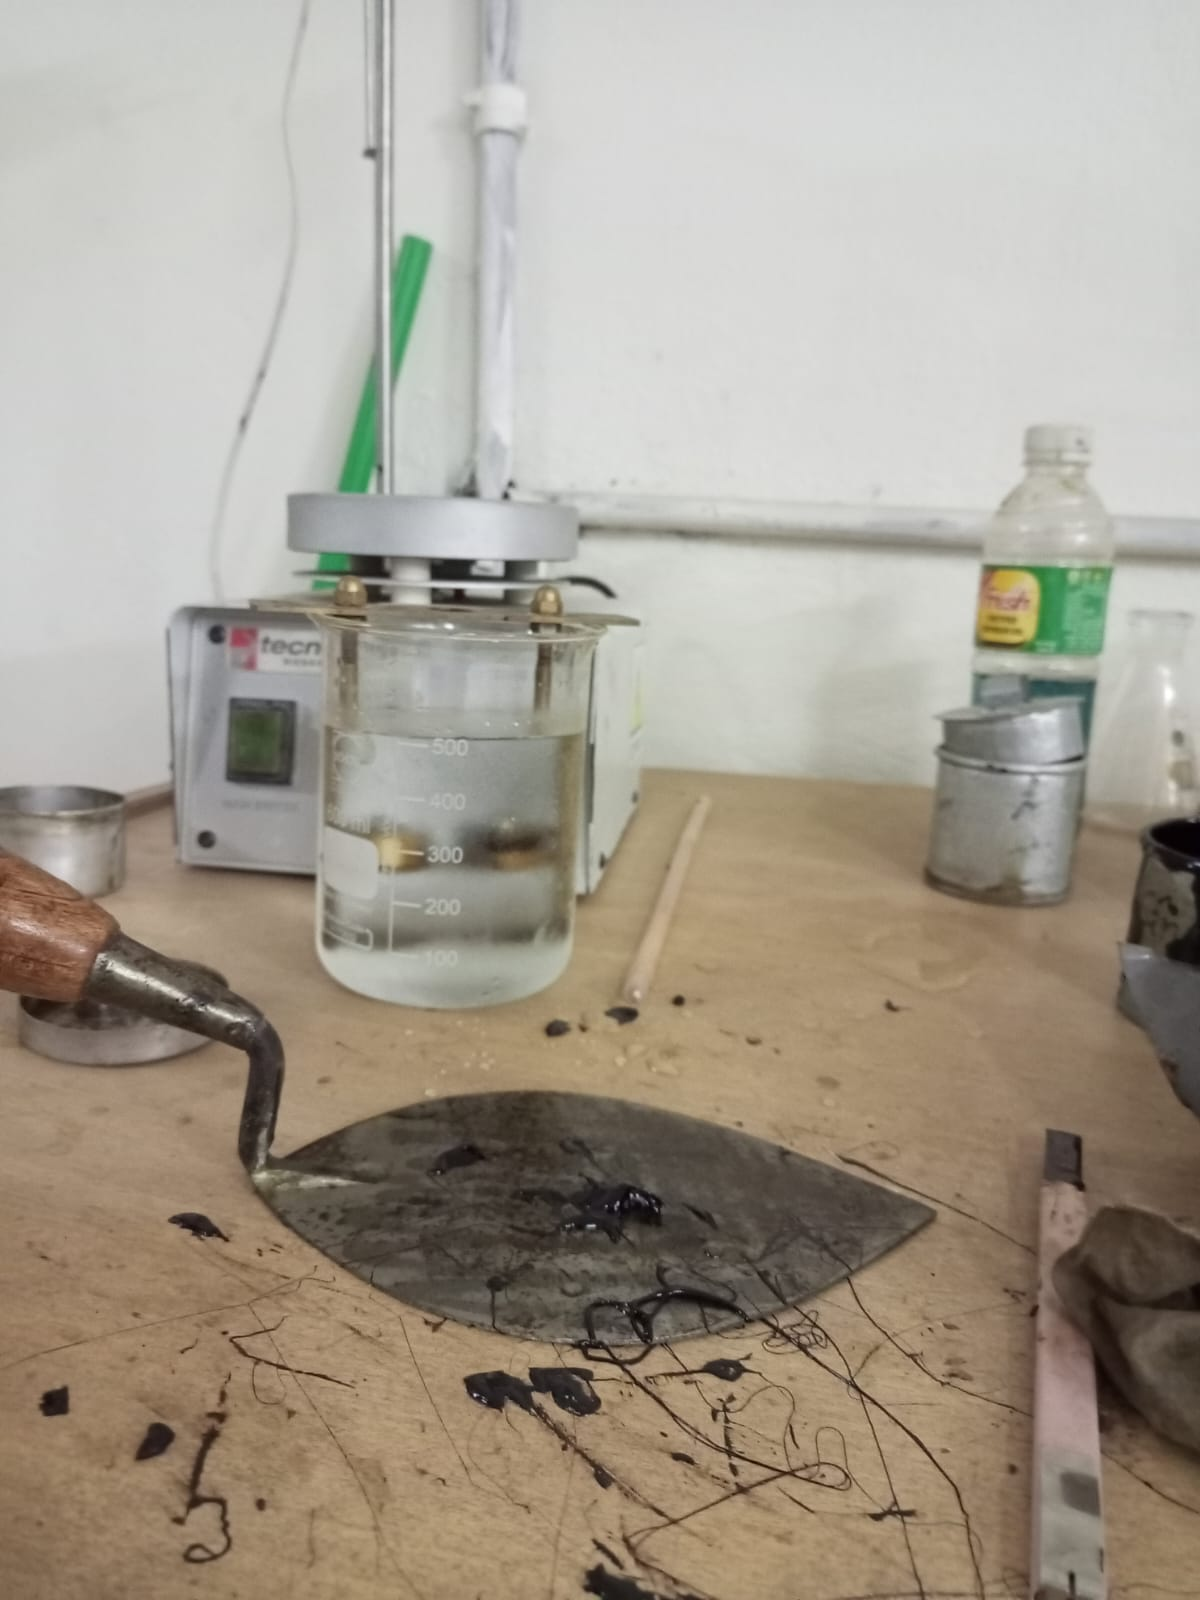
\includegraphics[width=4in, height=4in]{albums/appendix_16.jpeg}
\vspace{0.5cm}

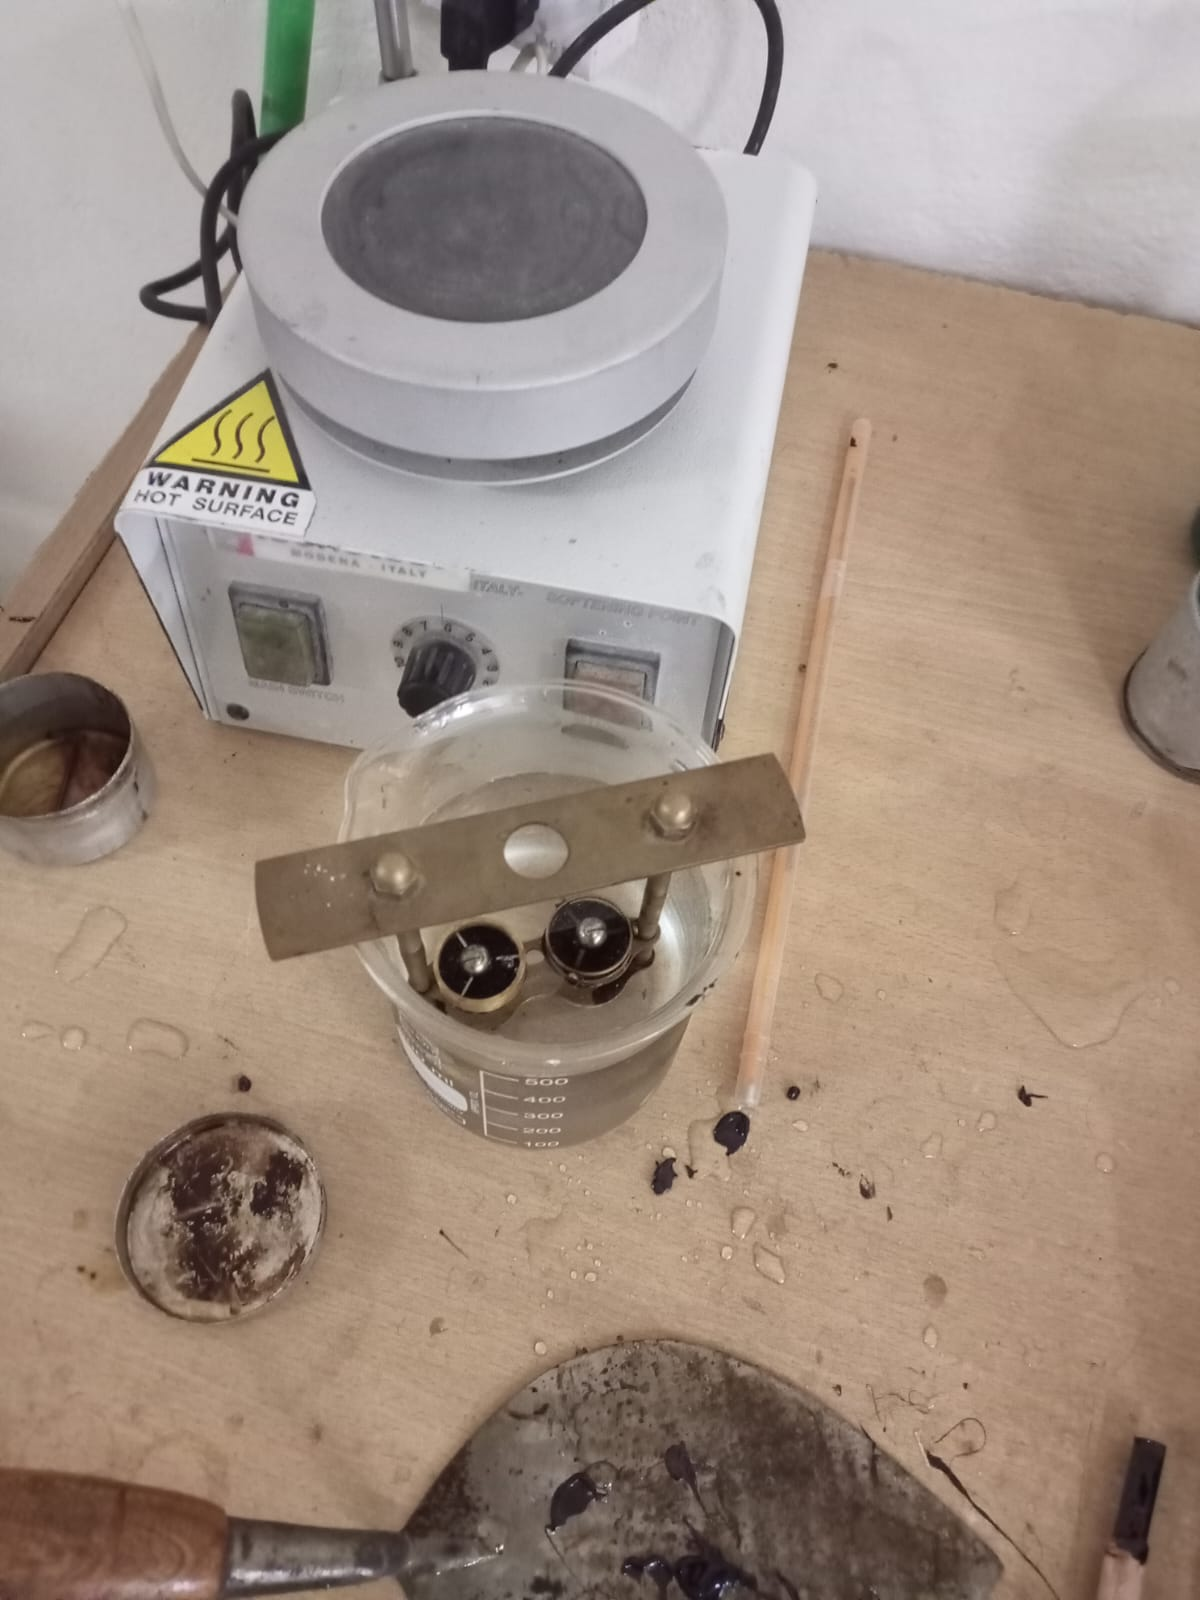
\includegraphics[width=4in, height=4in]{albums/appendix_17.jpeg}
\vspace{0.5cm}

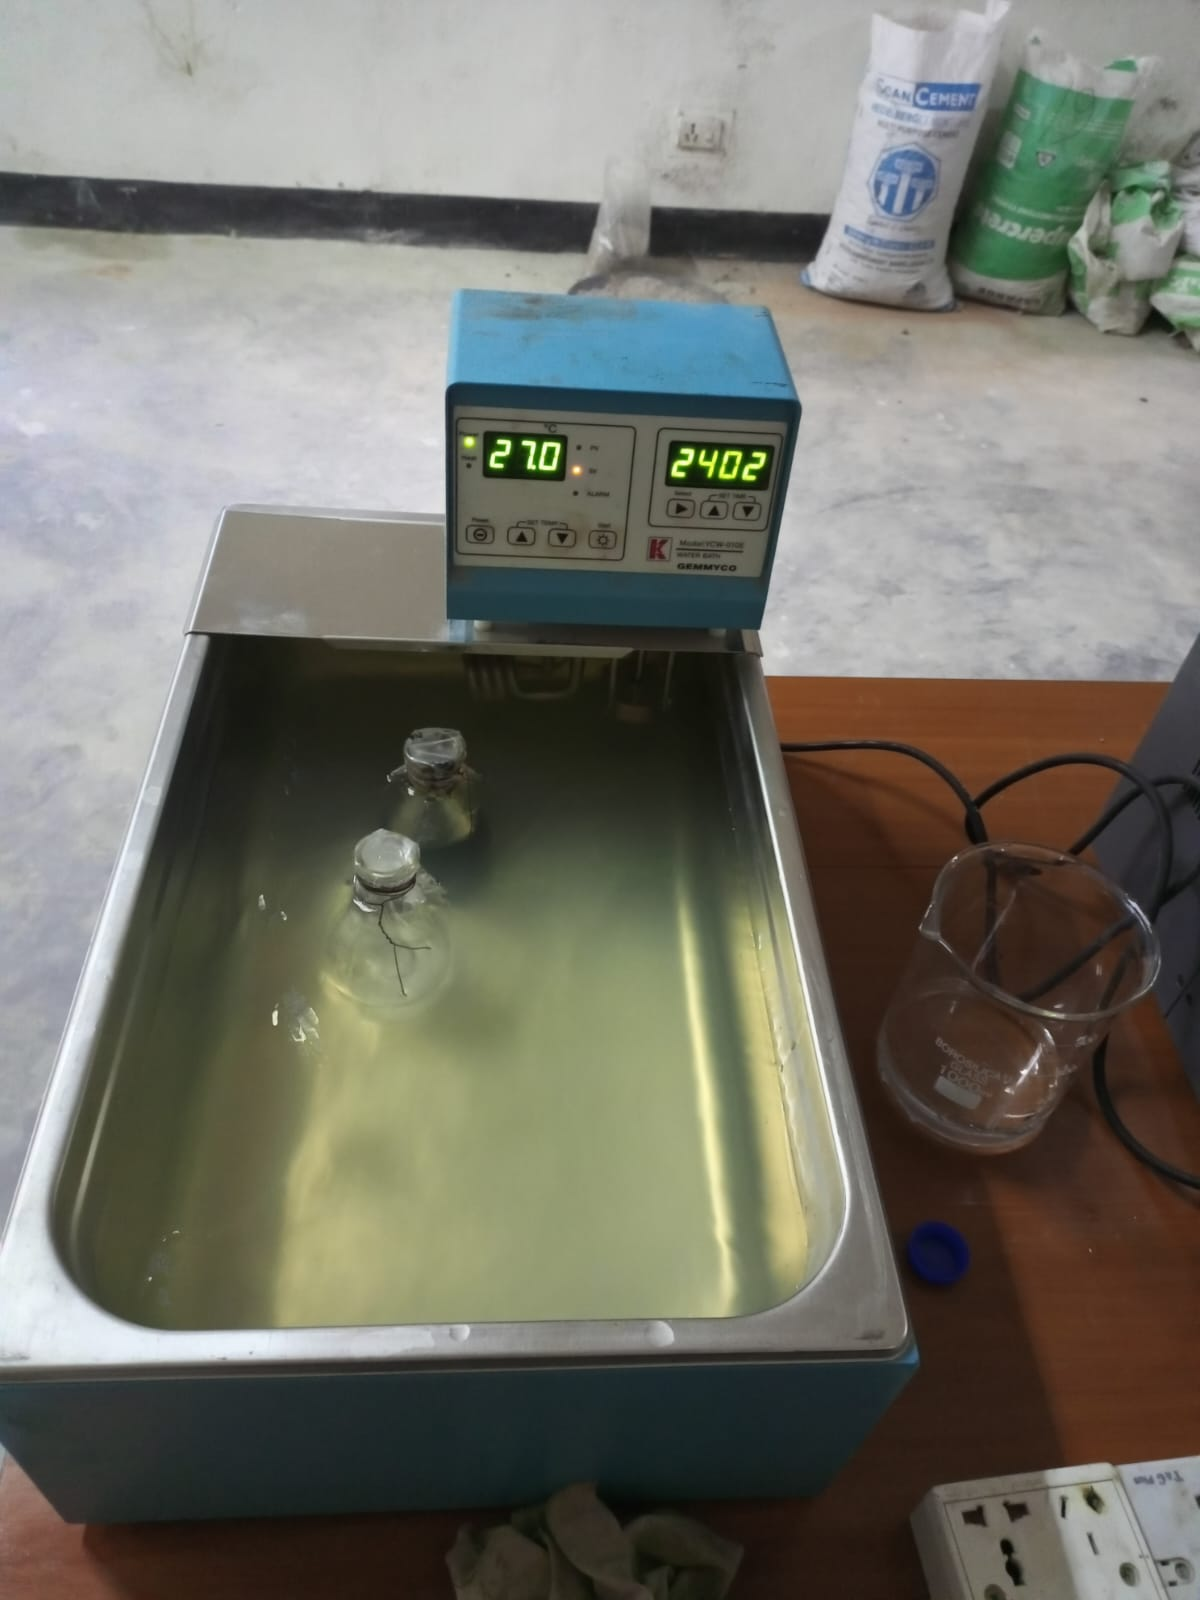
\includegraphics[width=4in, height=4in]{albums/appendix_18.jpeg}
\vspace{0.5cm}

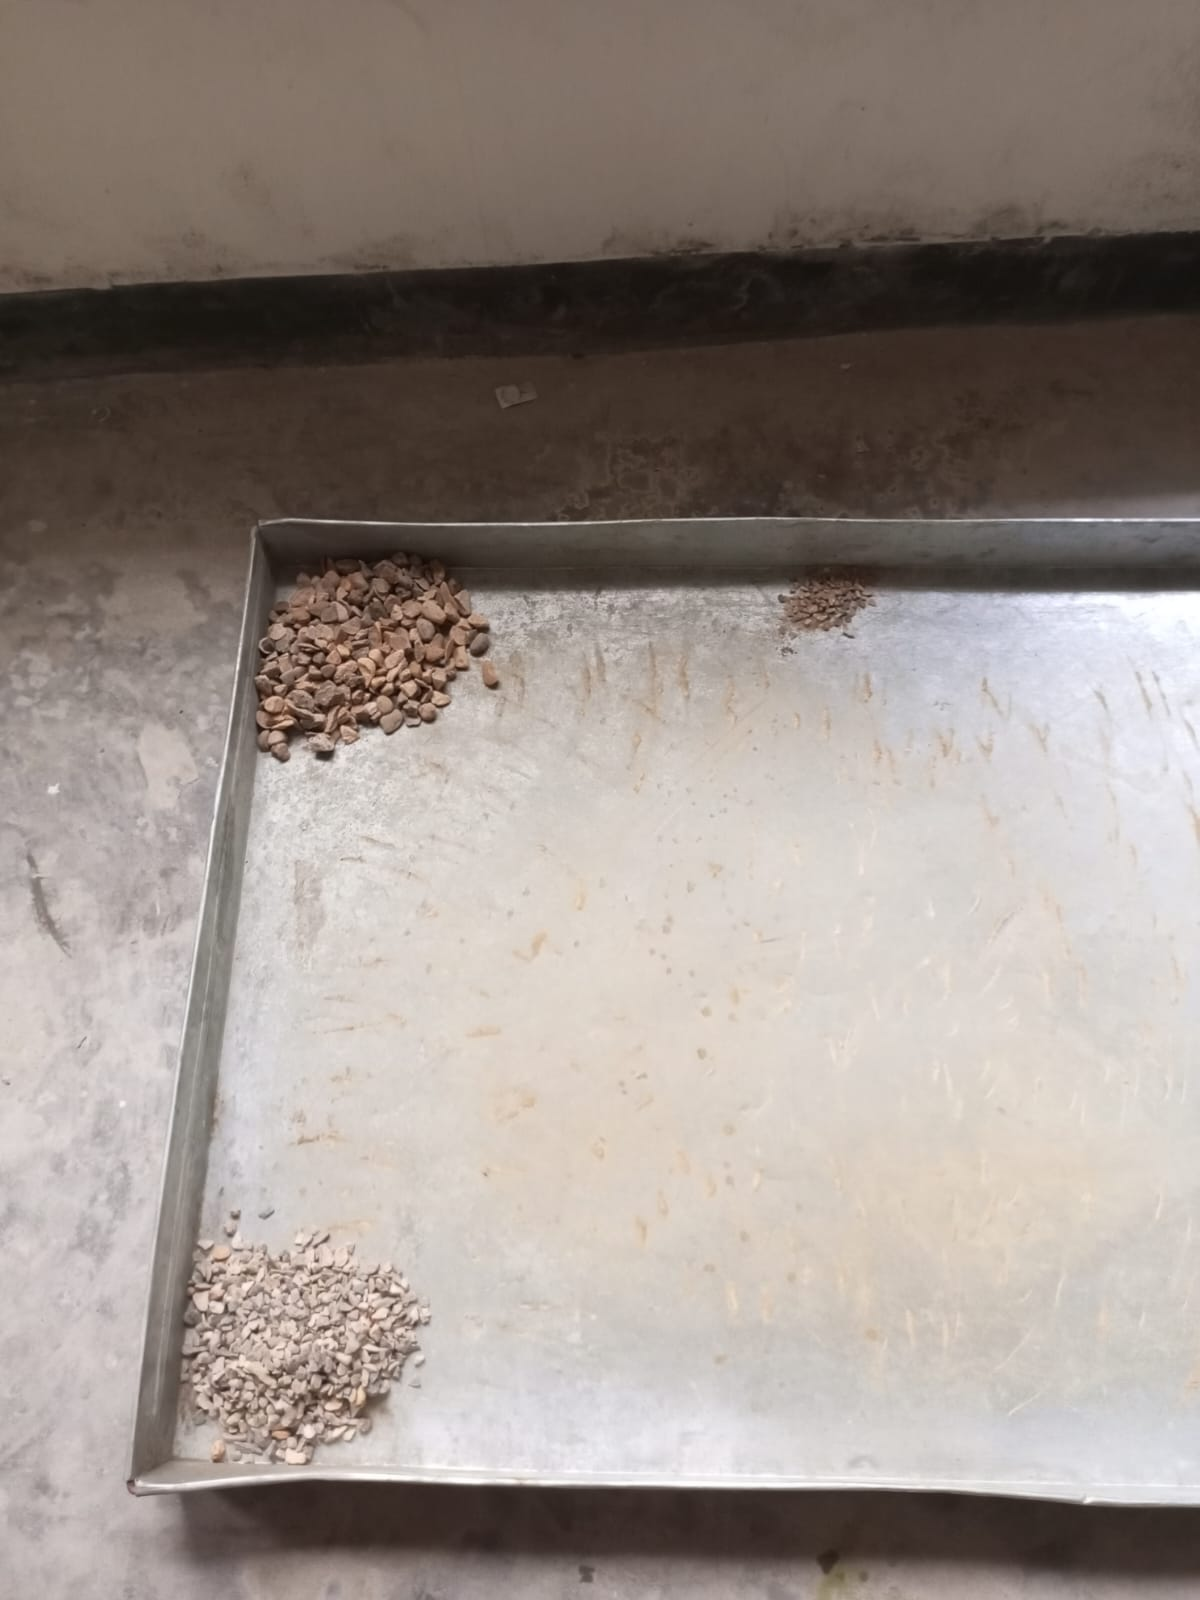
\includegraphics[width=4in, height=4in]{albums/appendix_19.jpeg}
\vspace{0.5cm}

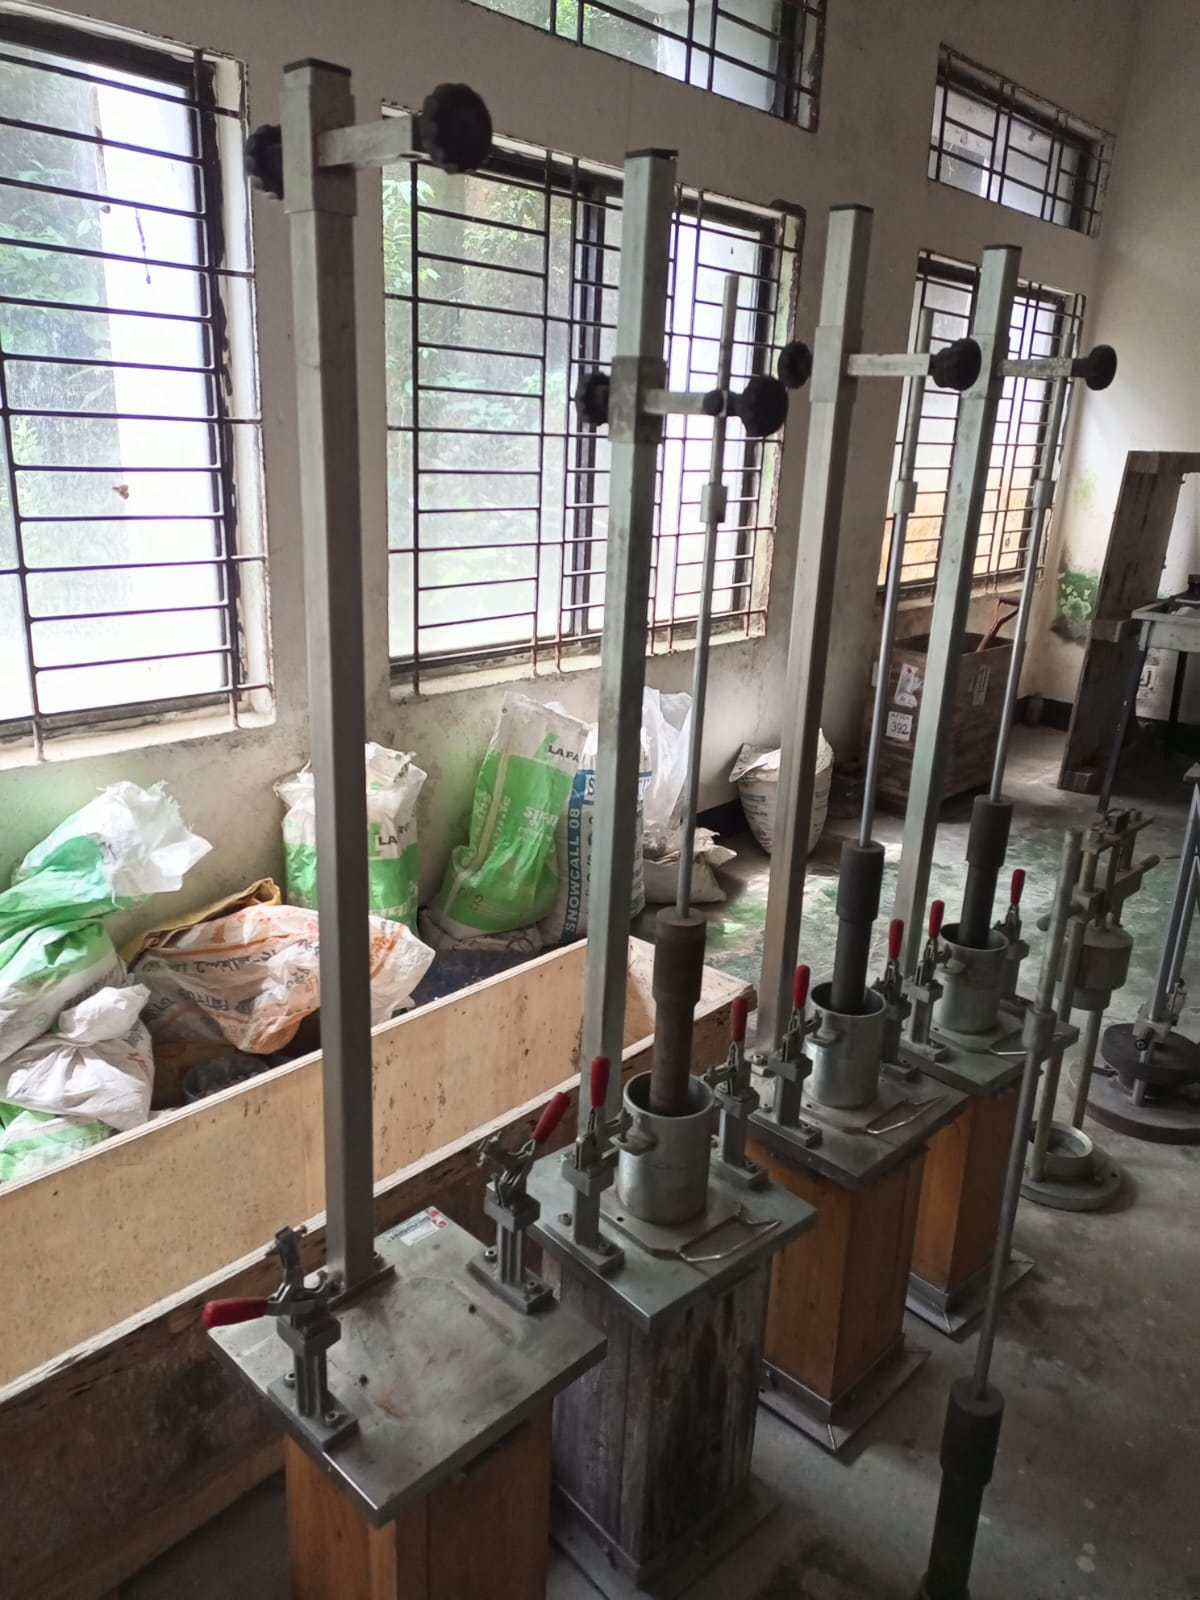
\includegraphics[width=4in, height=4in]{albums/appendix_20.jpeg}
\vspace{0.5cm}

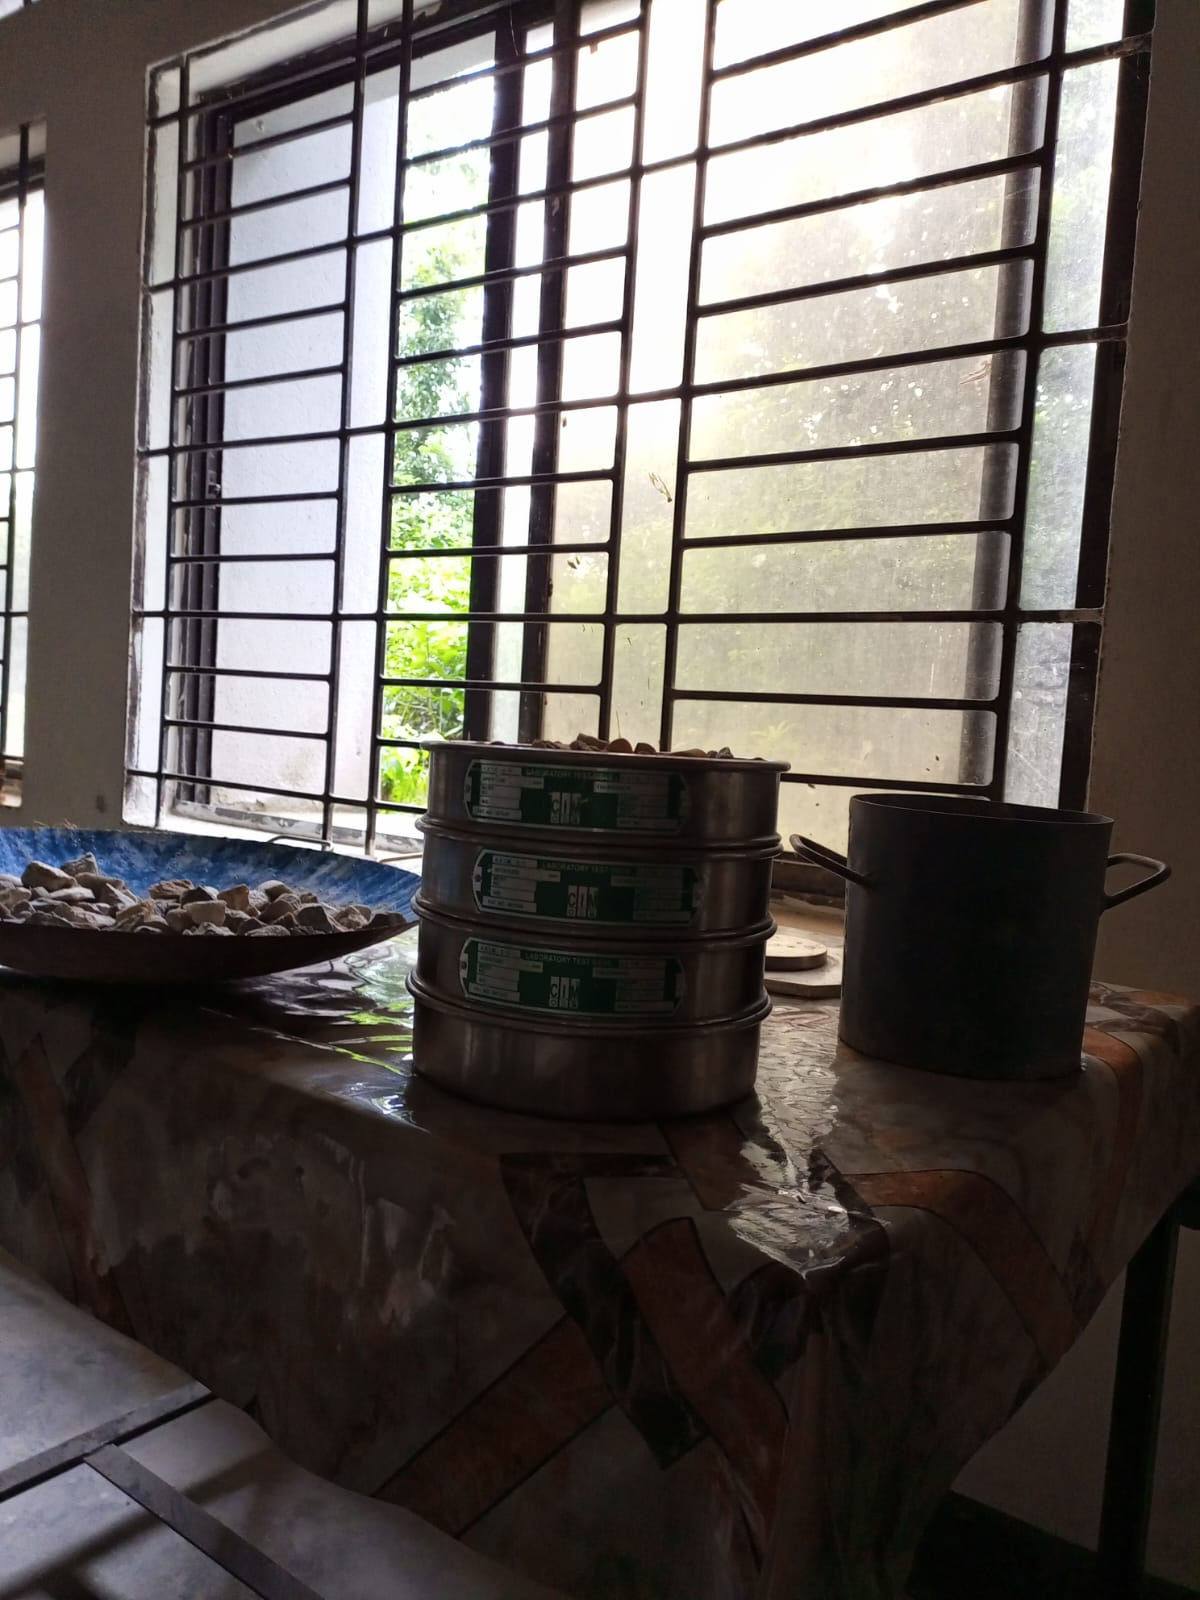
\includegraphics[width=4in, height=4in]{albums/appendix_21.jpeg}
\vspace{0.5cm}

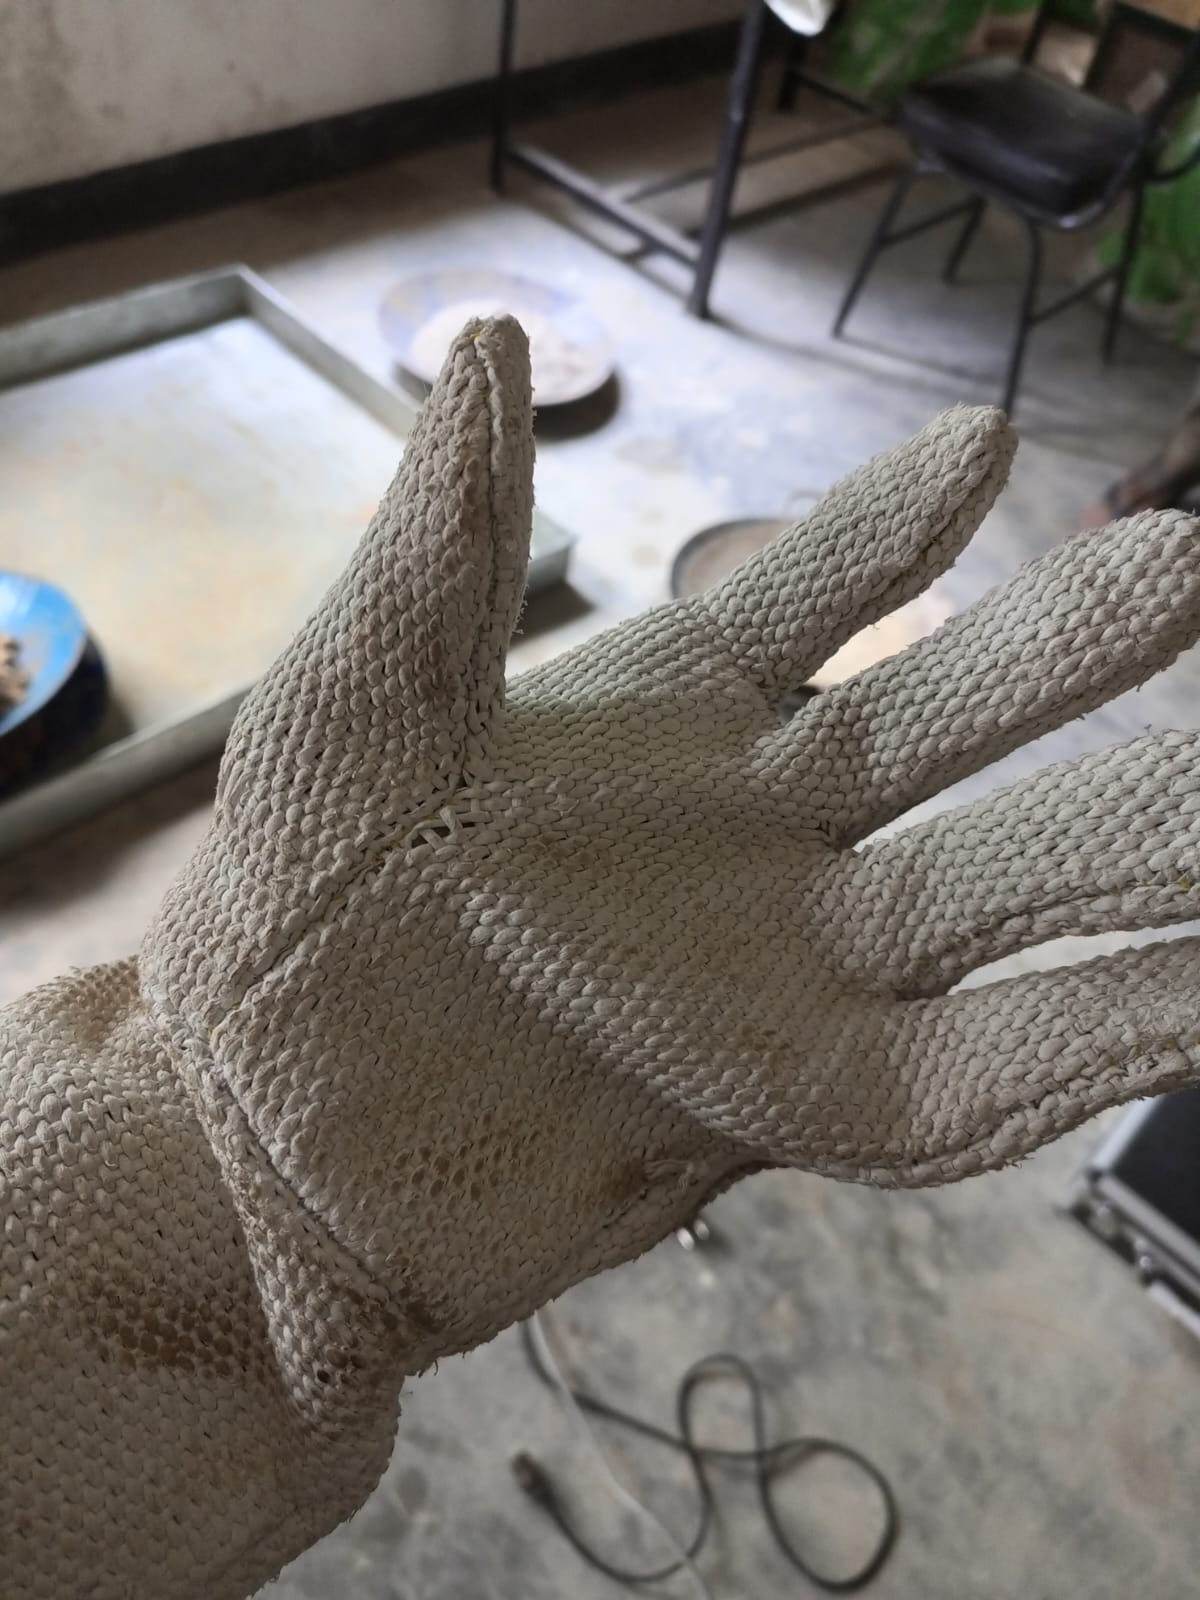
\includegraphics[width=4in, height=4in]{albums/appendix_22.jpeg}
\vspace{0.5cm}

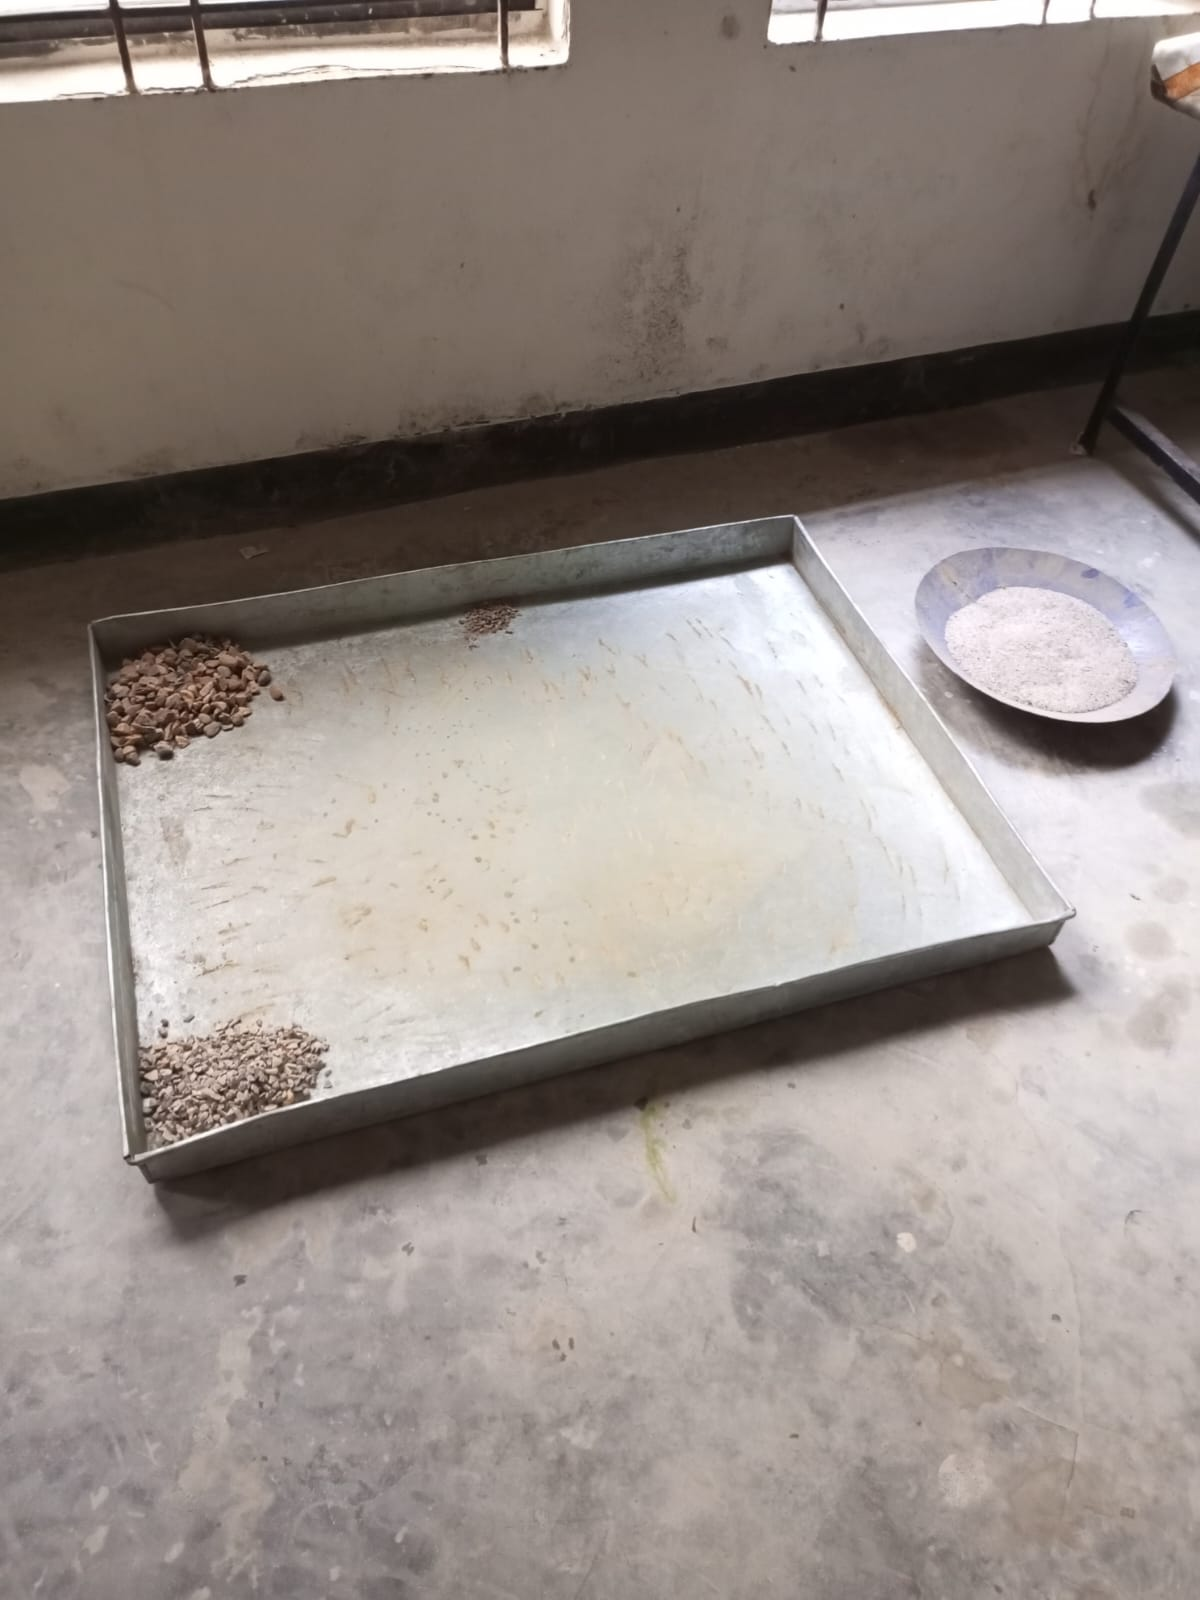
\includegraphics[width=4in, height=4in]{albums/appendix_23.jpeg}
\vspace{0.5cm}

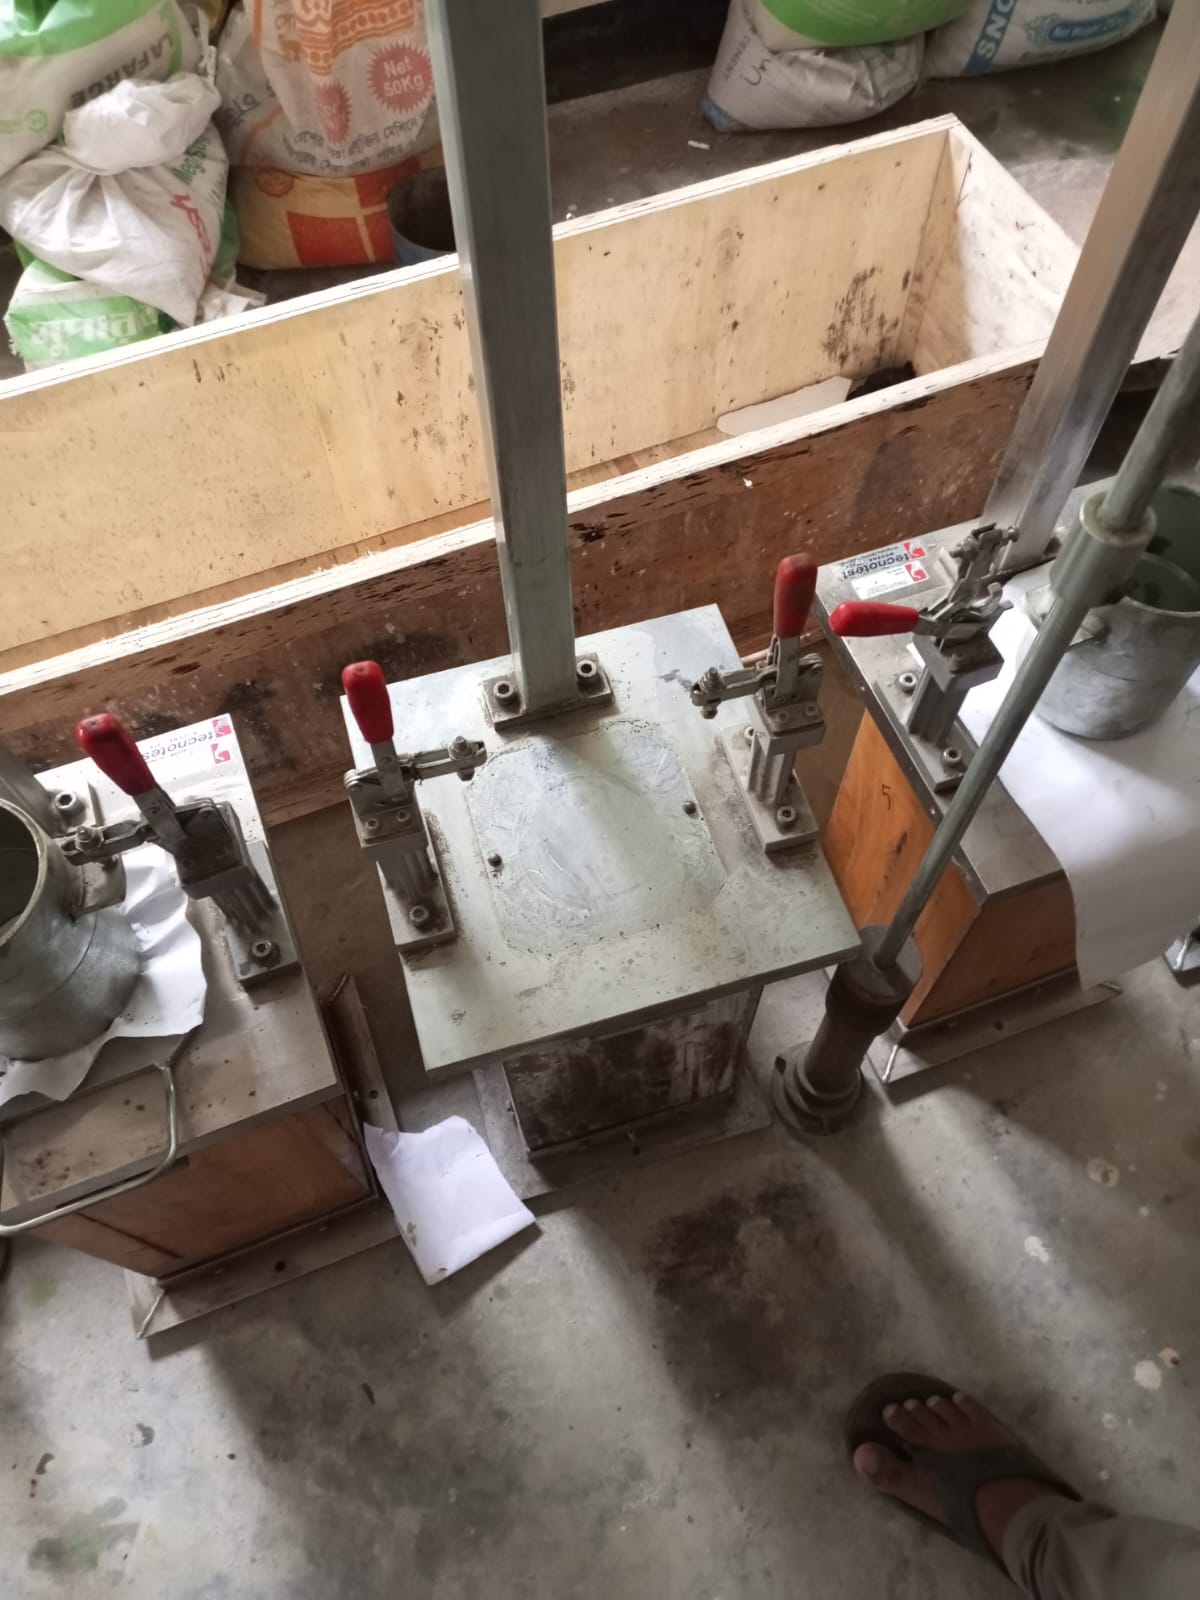
\includegraphics[width=4in, height=4in]{albums/appendix_24.jpeg}
\vspace{0.5cm}

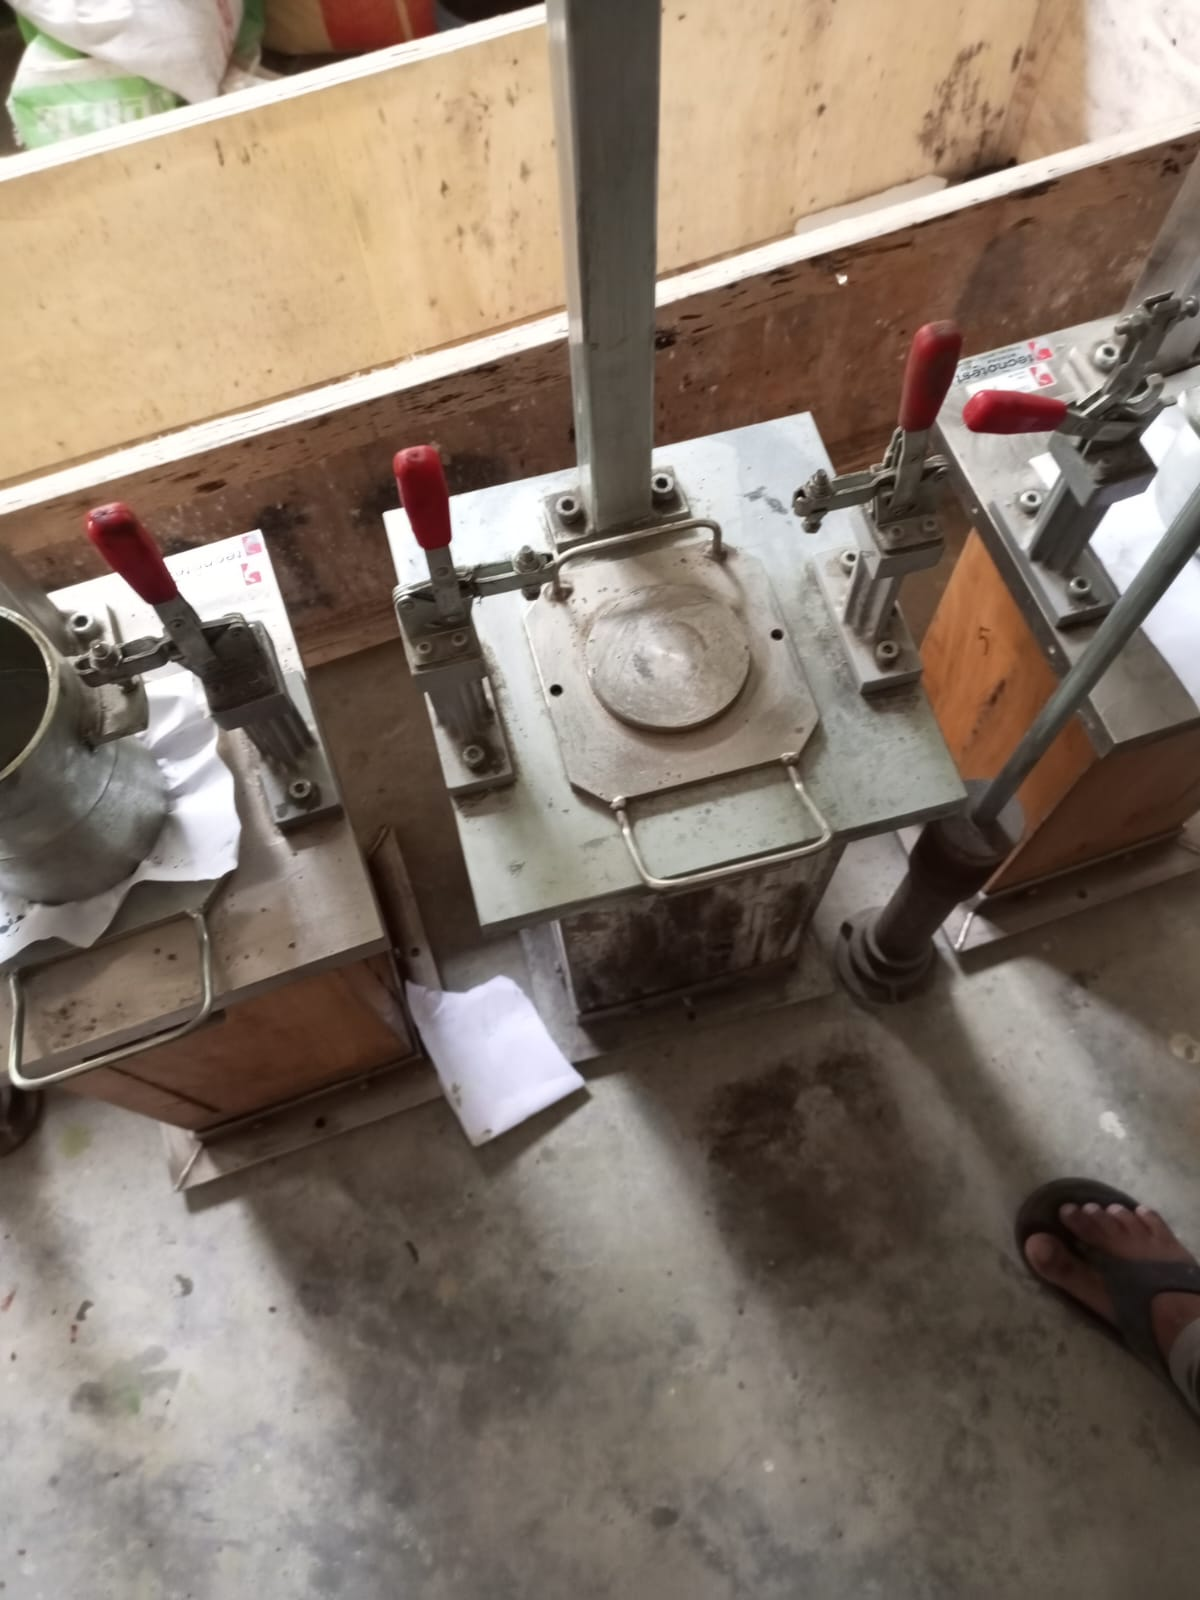
\includegraphics[width=4in, height=4in]{albums/appendix_25.jpeg}
\vspace{0.5cm}

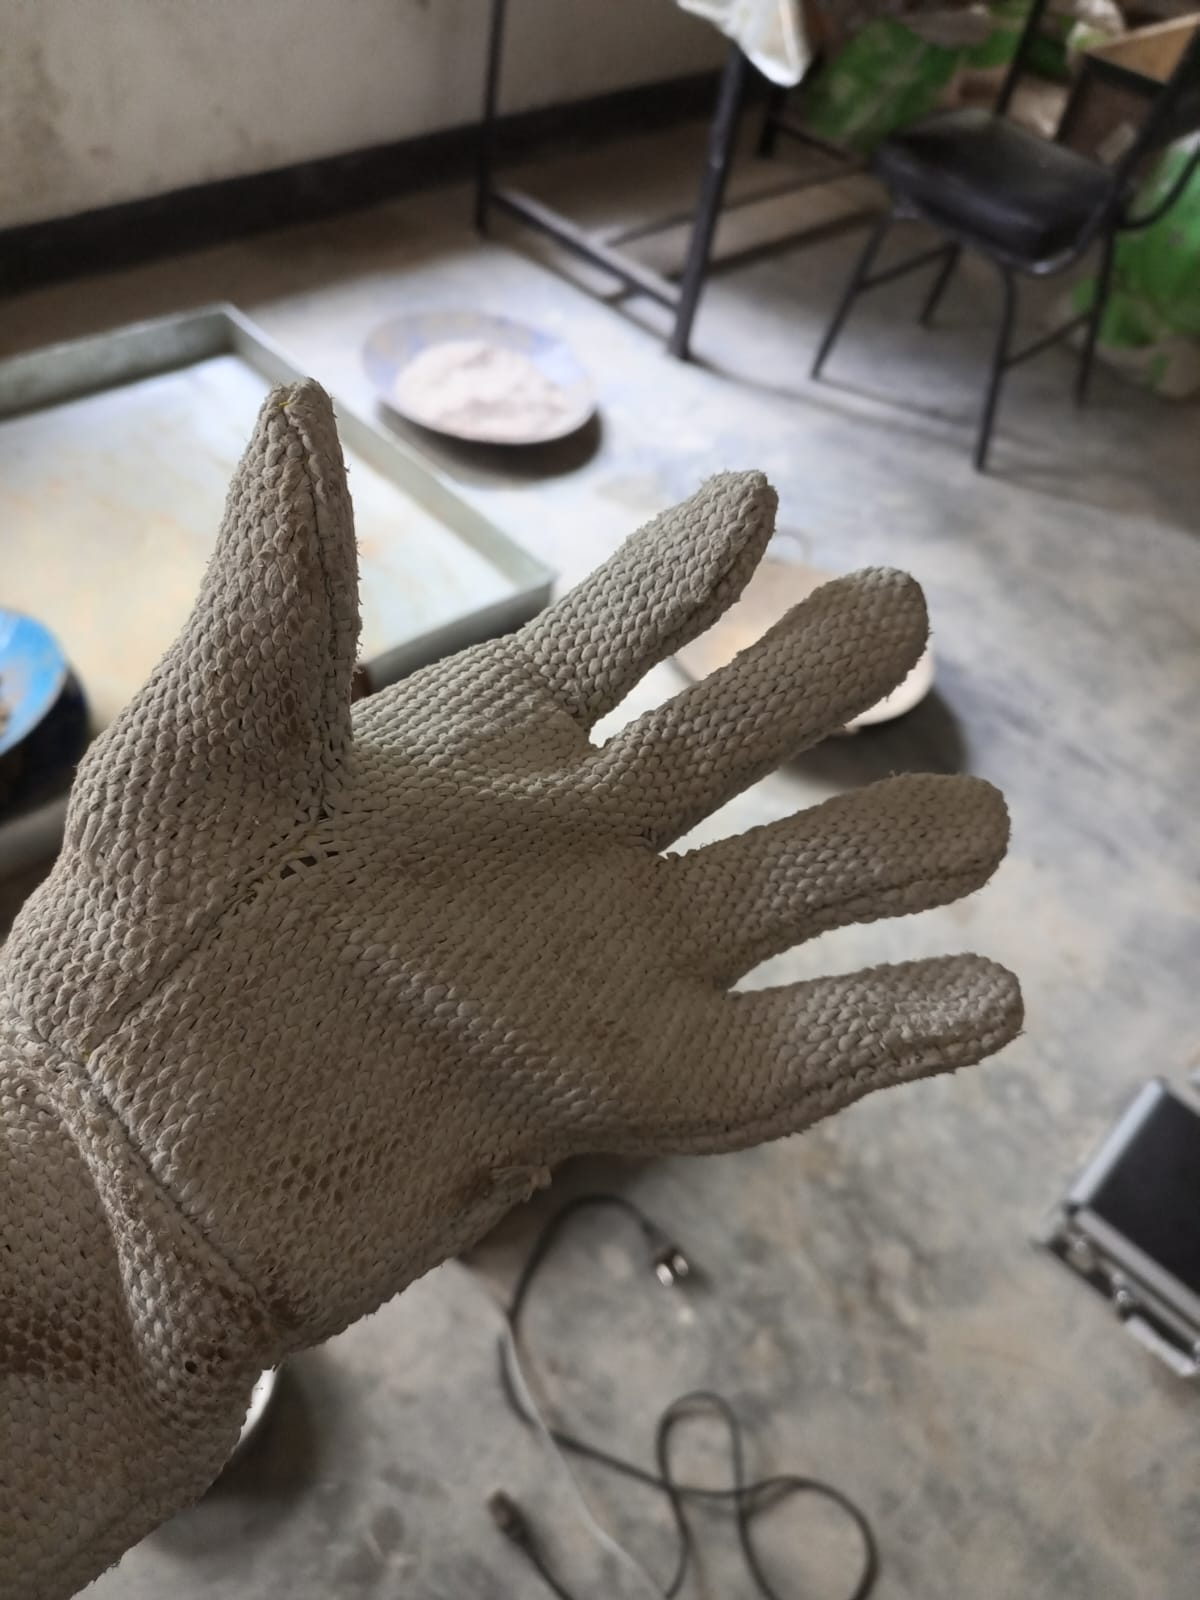
\includegraphics[width=4in, height=4in]{albums/appendix_26.jpeg}
\vspace{0.5cm}

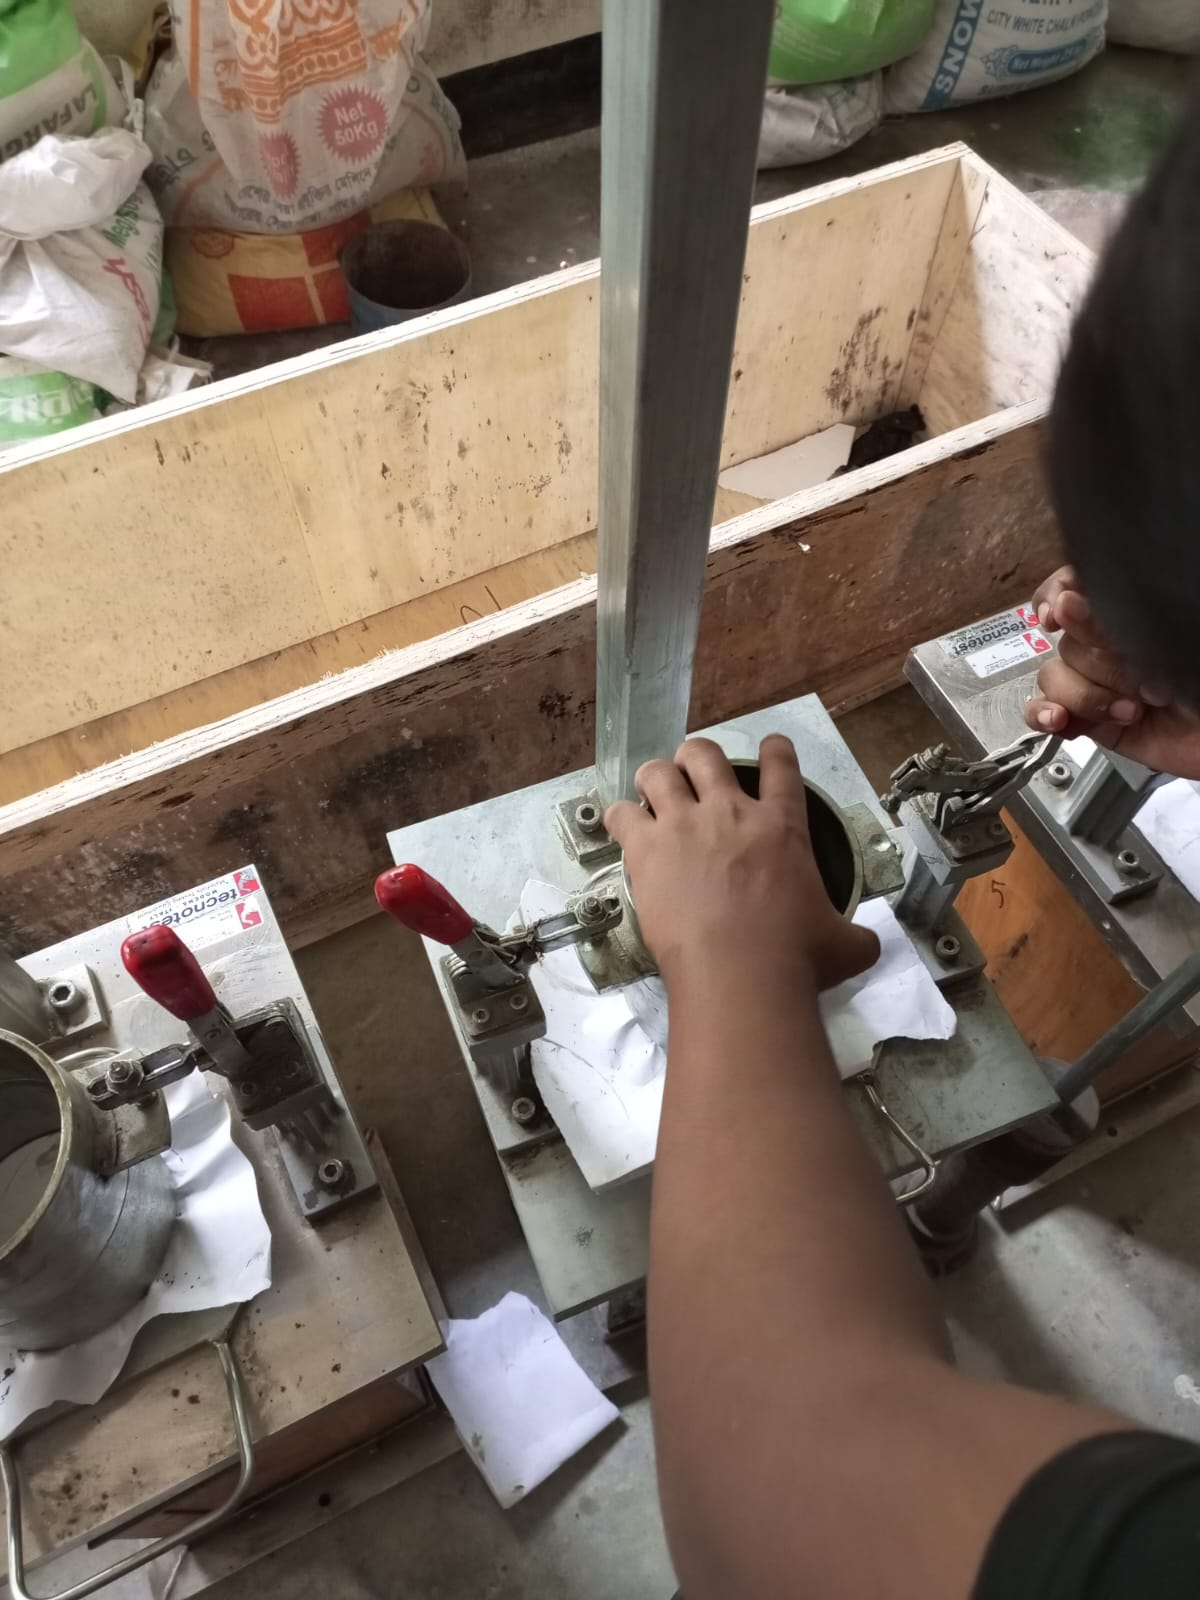
\includegraphics[width=4in, height=4in]{albums/appendix_27.jpeg}
\vspace{0.5cm}

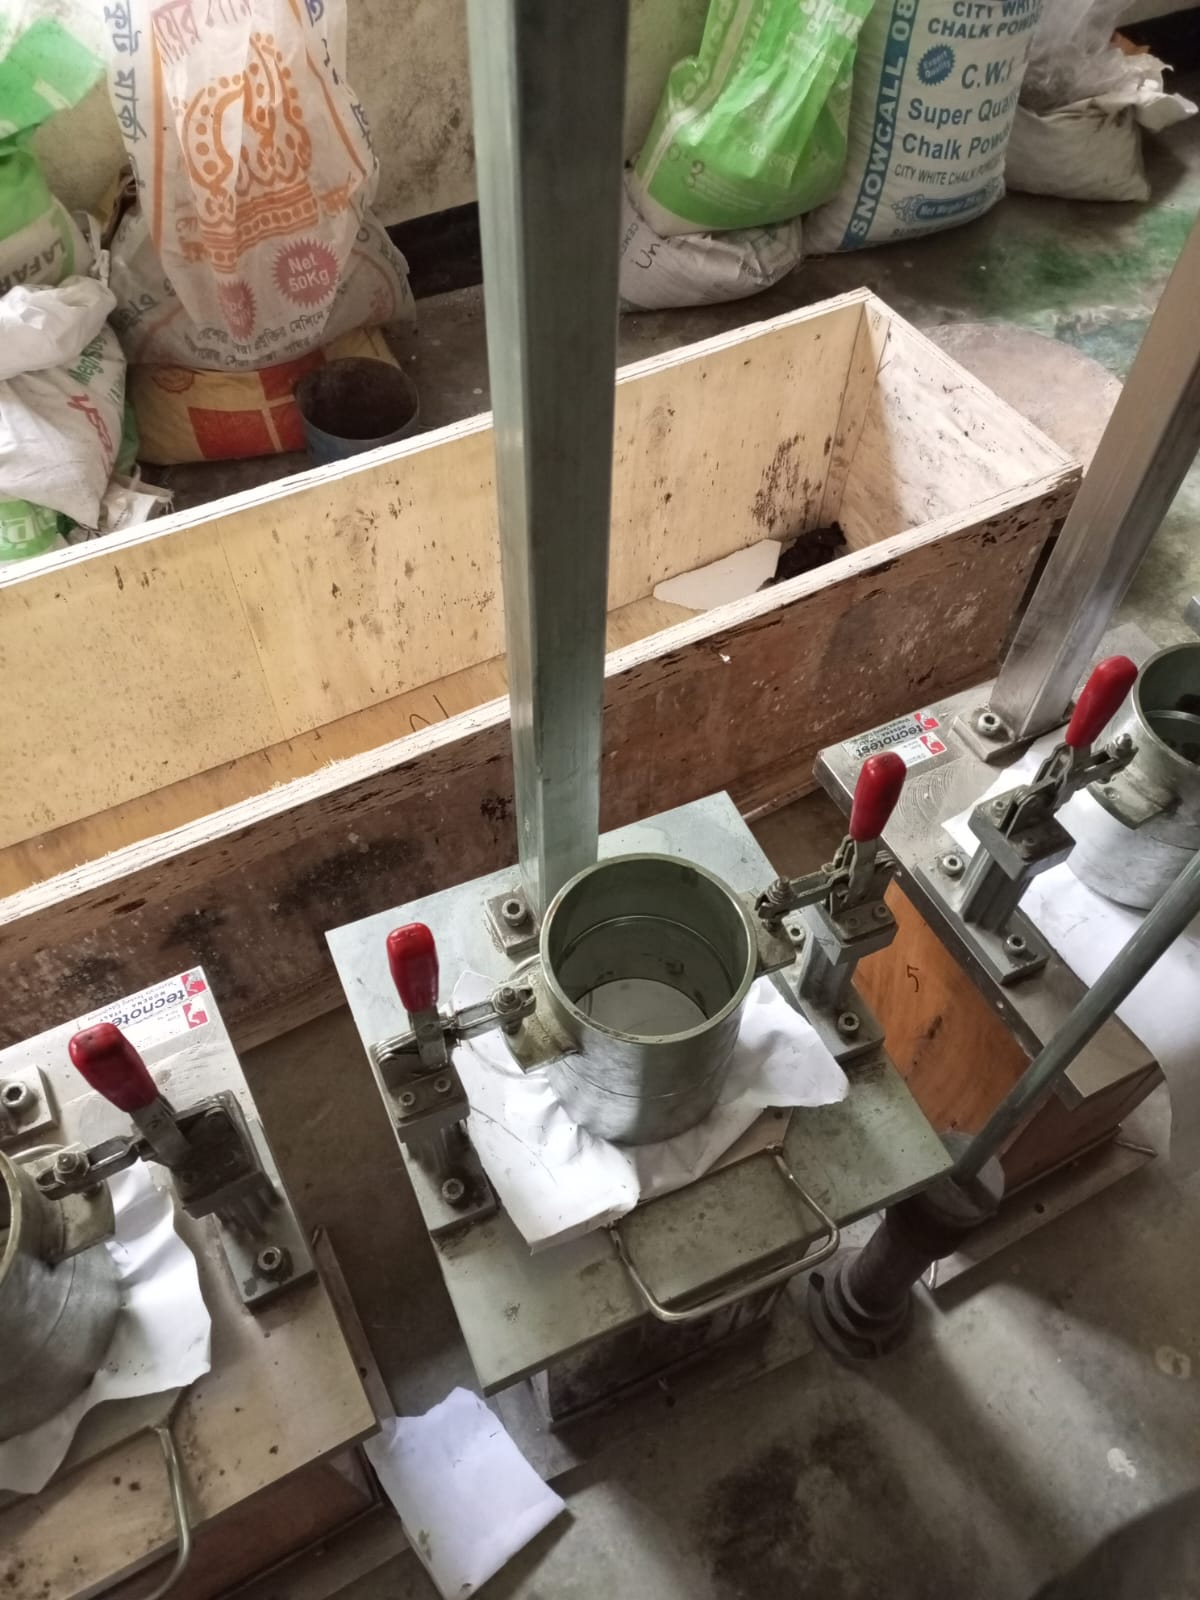
\includegraphics[width=4in, height=4in]{albums/appendix_28.jpeg}
\vspace{0.5cm}

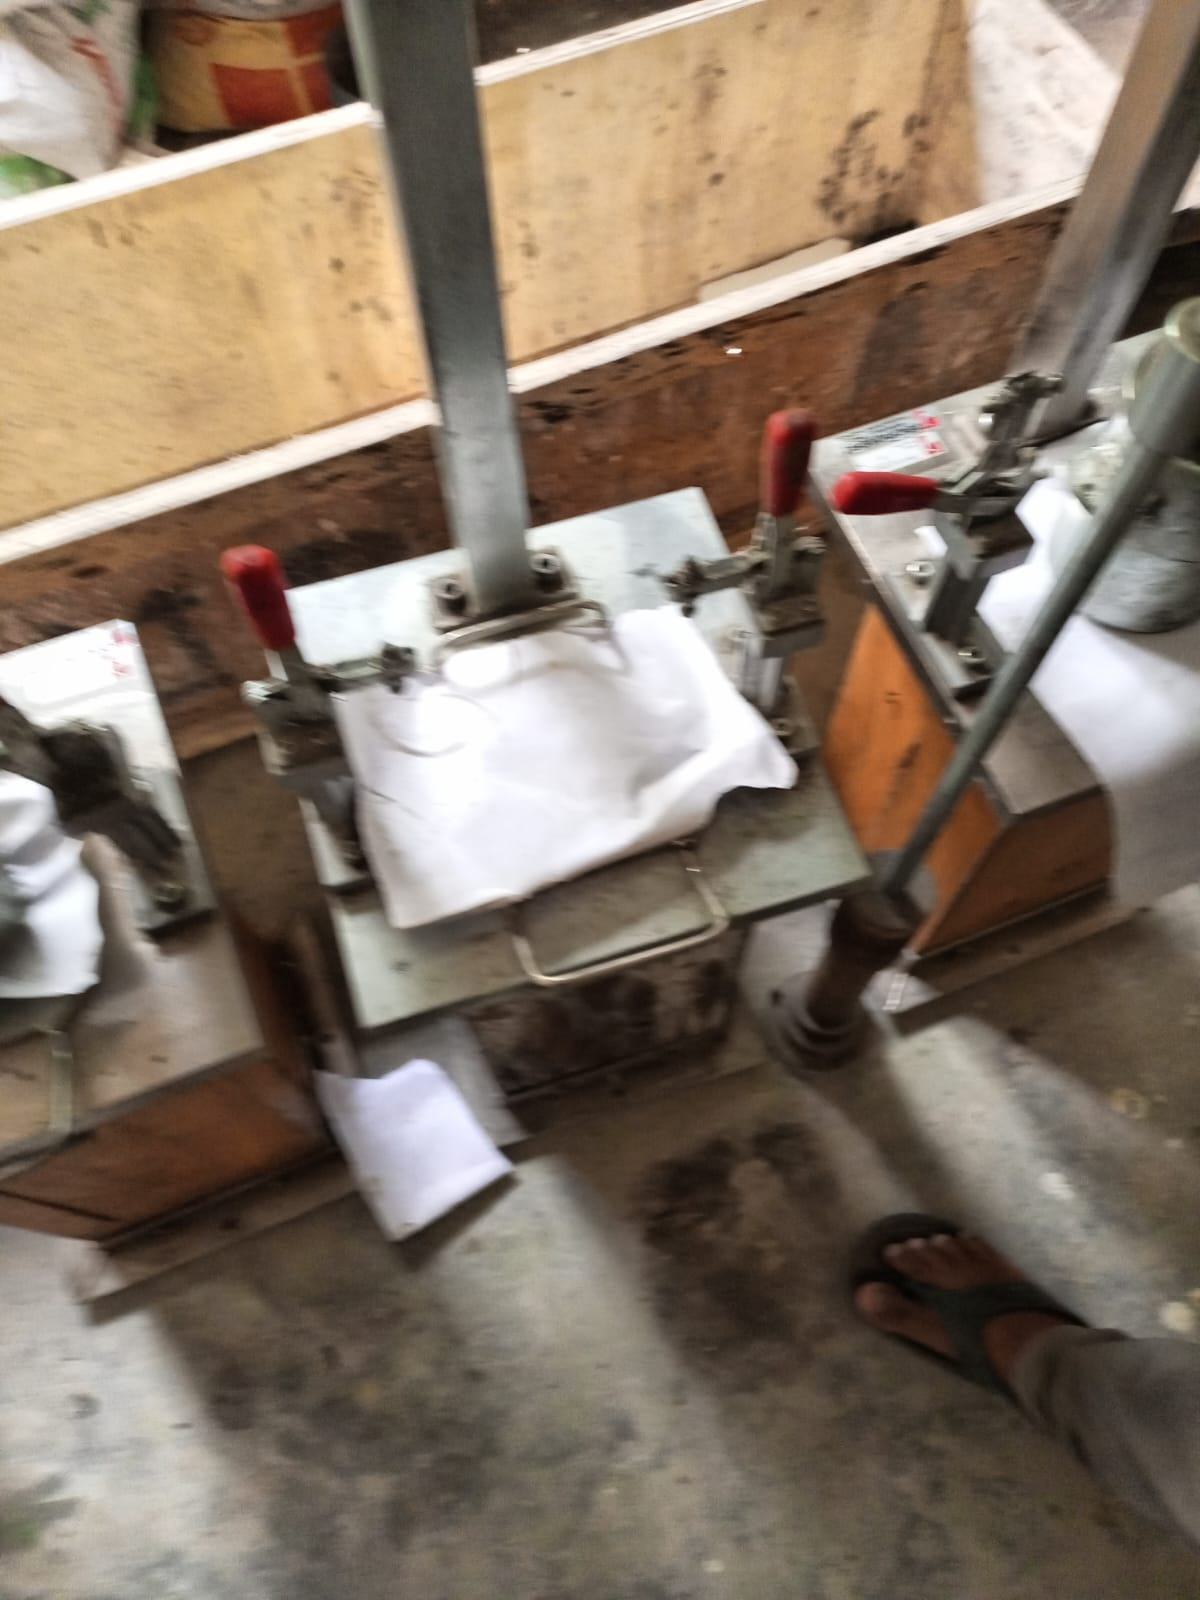
\includegraphics[width=4in, height=4in]{albums/appendix_29.jpeg}
\vspace{0.5cm}

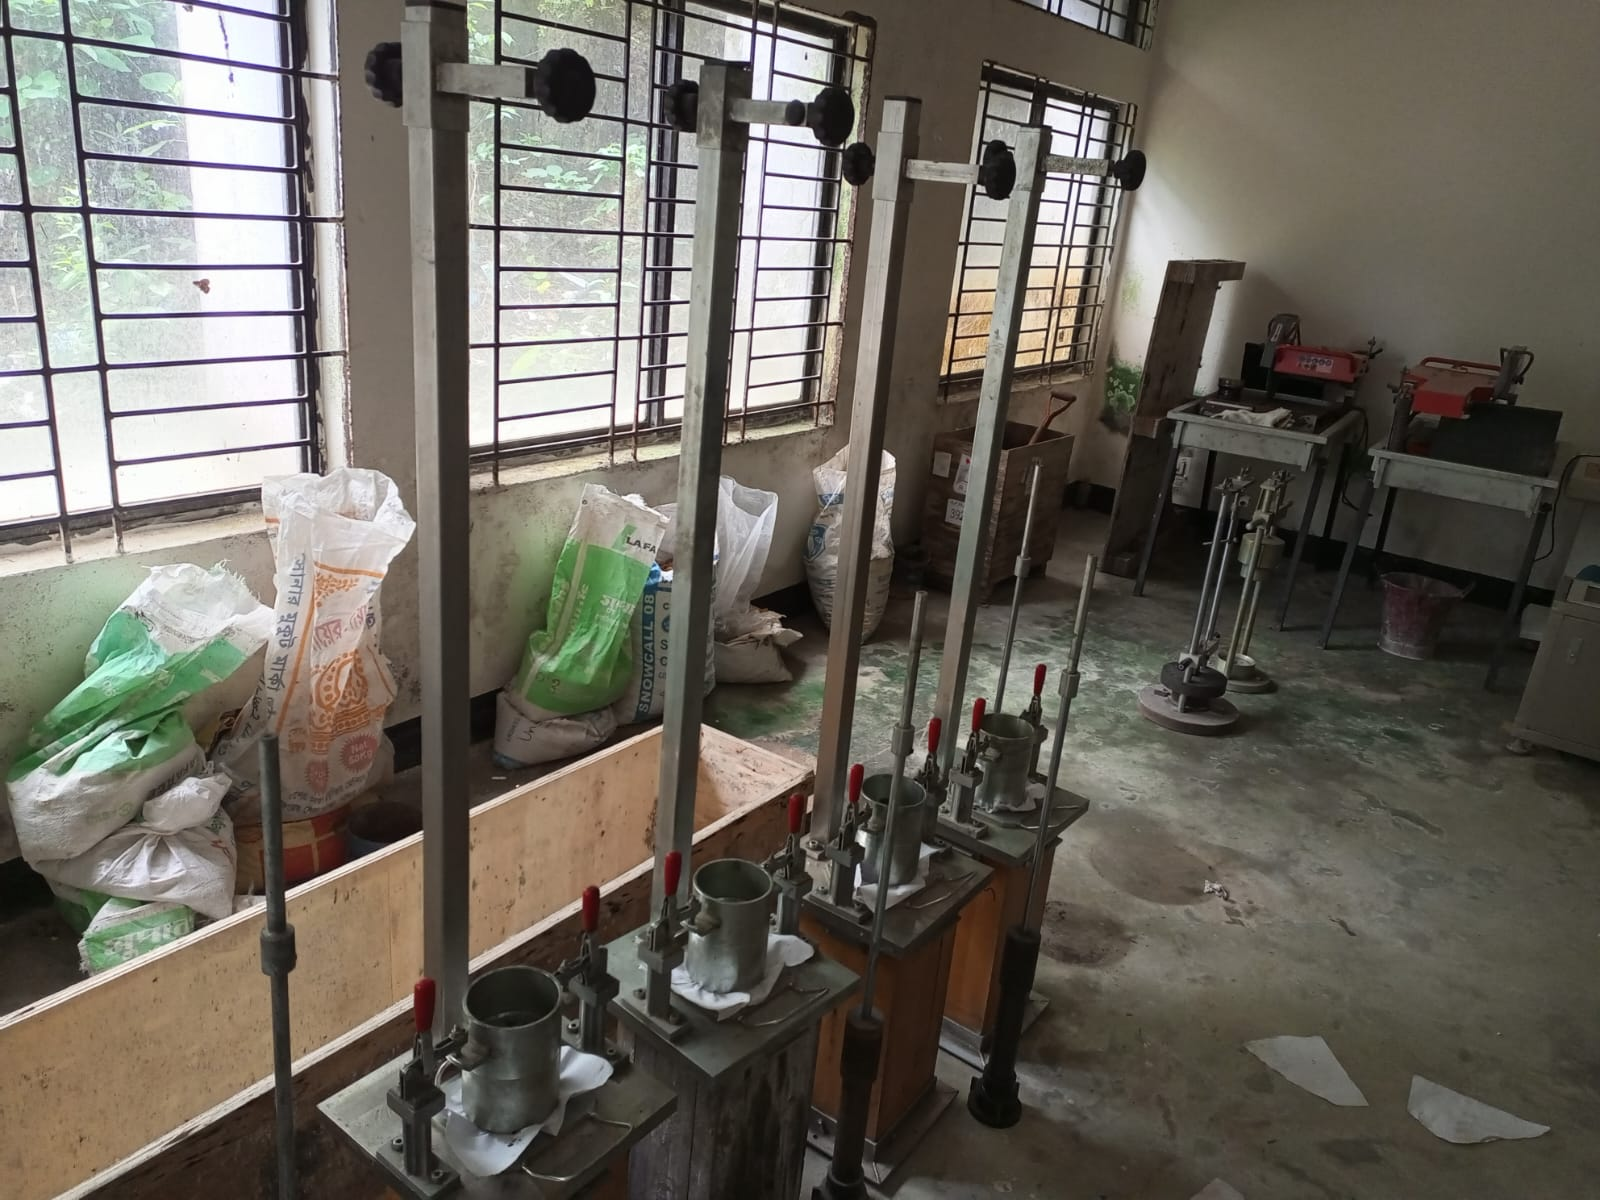
\includegraphics[width=4in, height=4in]{albums/appendix_30.jpeg}
\vspace{0.5cm}

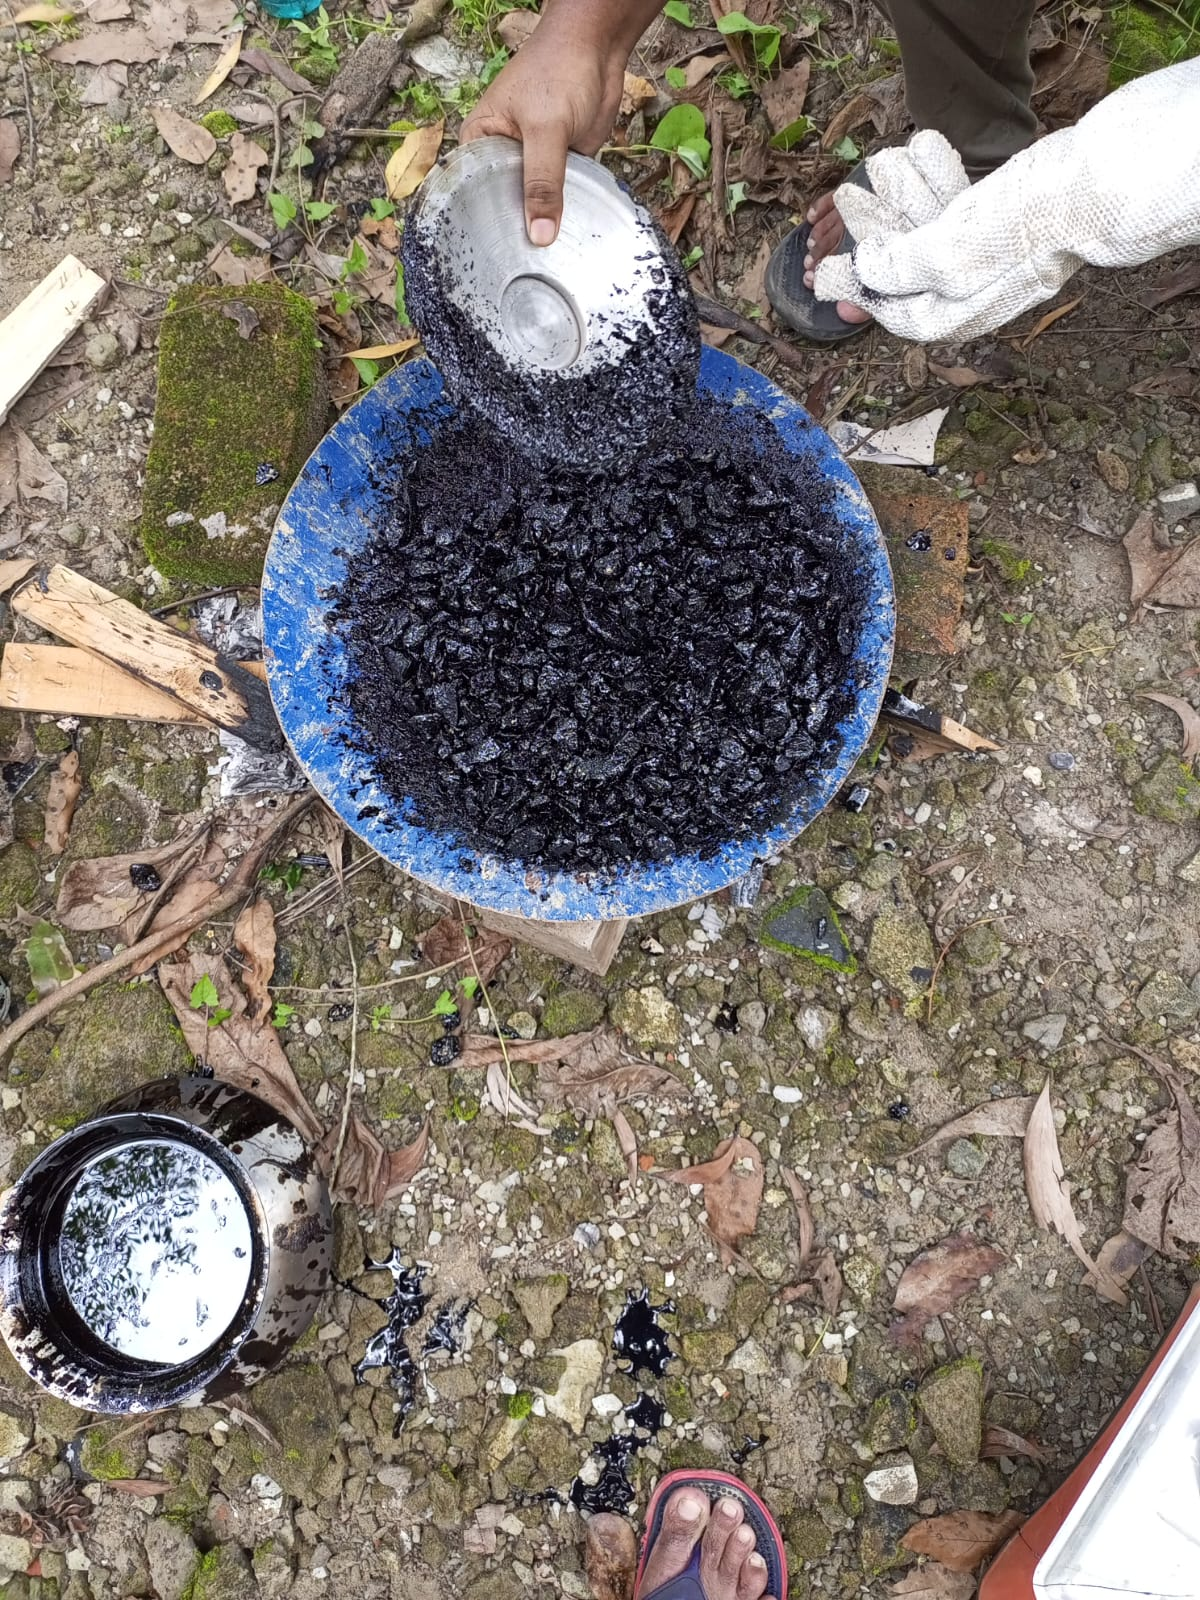
\includegraphics[width=4in, height=4in]{albums/appendix_31.jpeg}
\vspace{0.5cm}

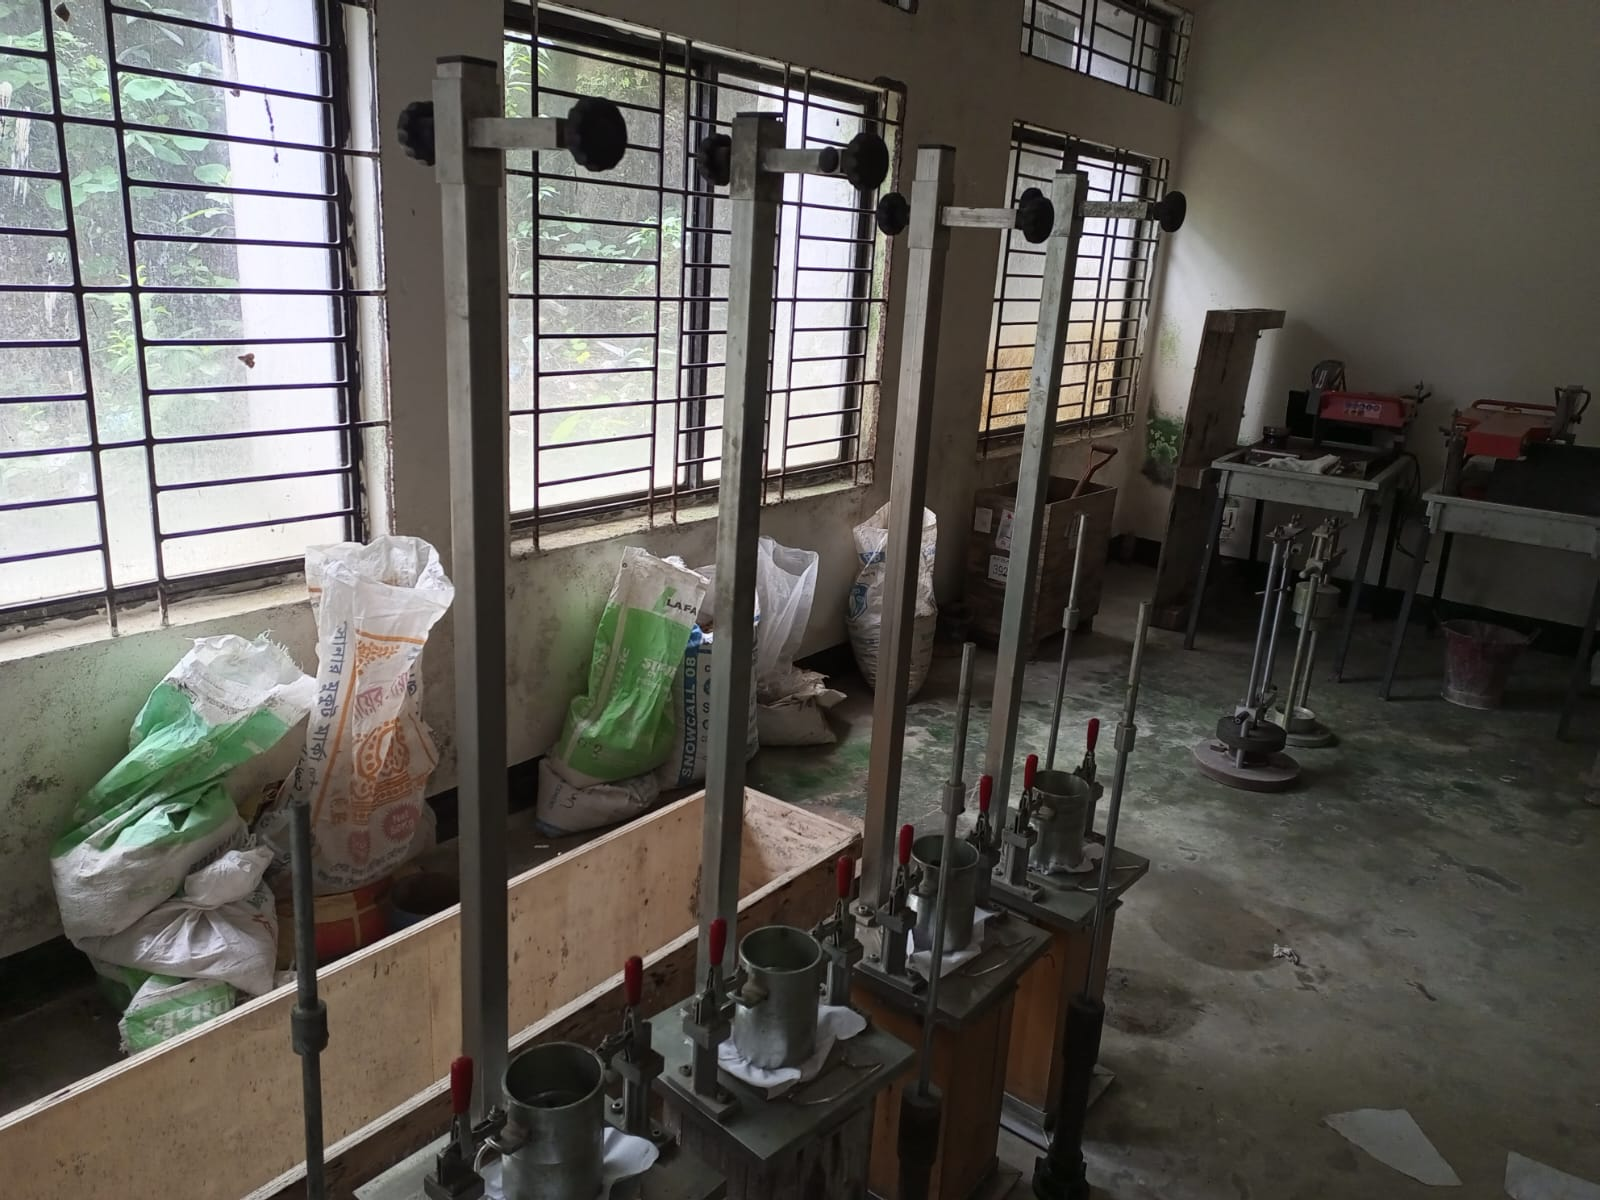
\includegraphics[width=4in, height=4in]{albums/appendix_32.jpeg}
\vspace{0.5cm}

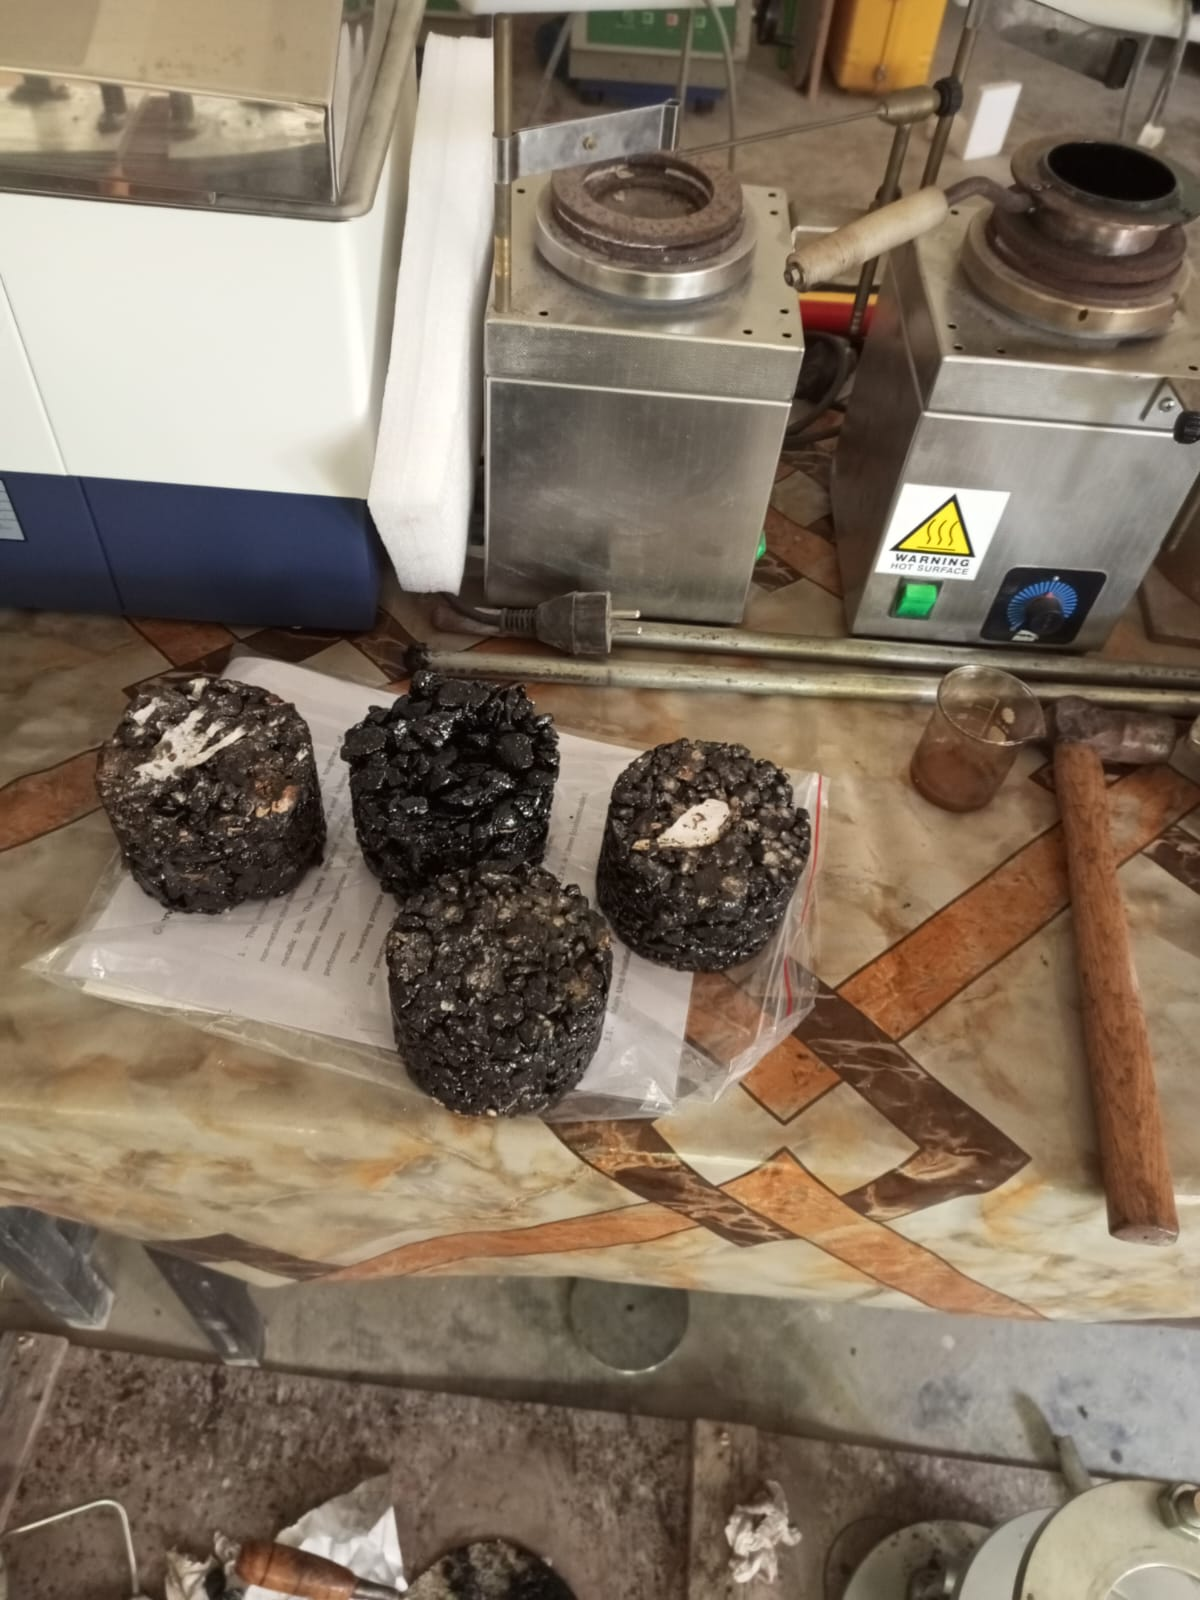
\includegraphics[width=4in, height=4in]{albums/appendix_33.jpeg}
\vspace{0.5cm}

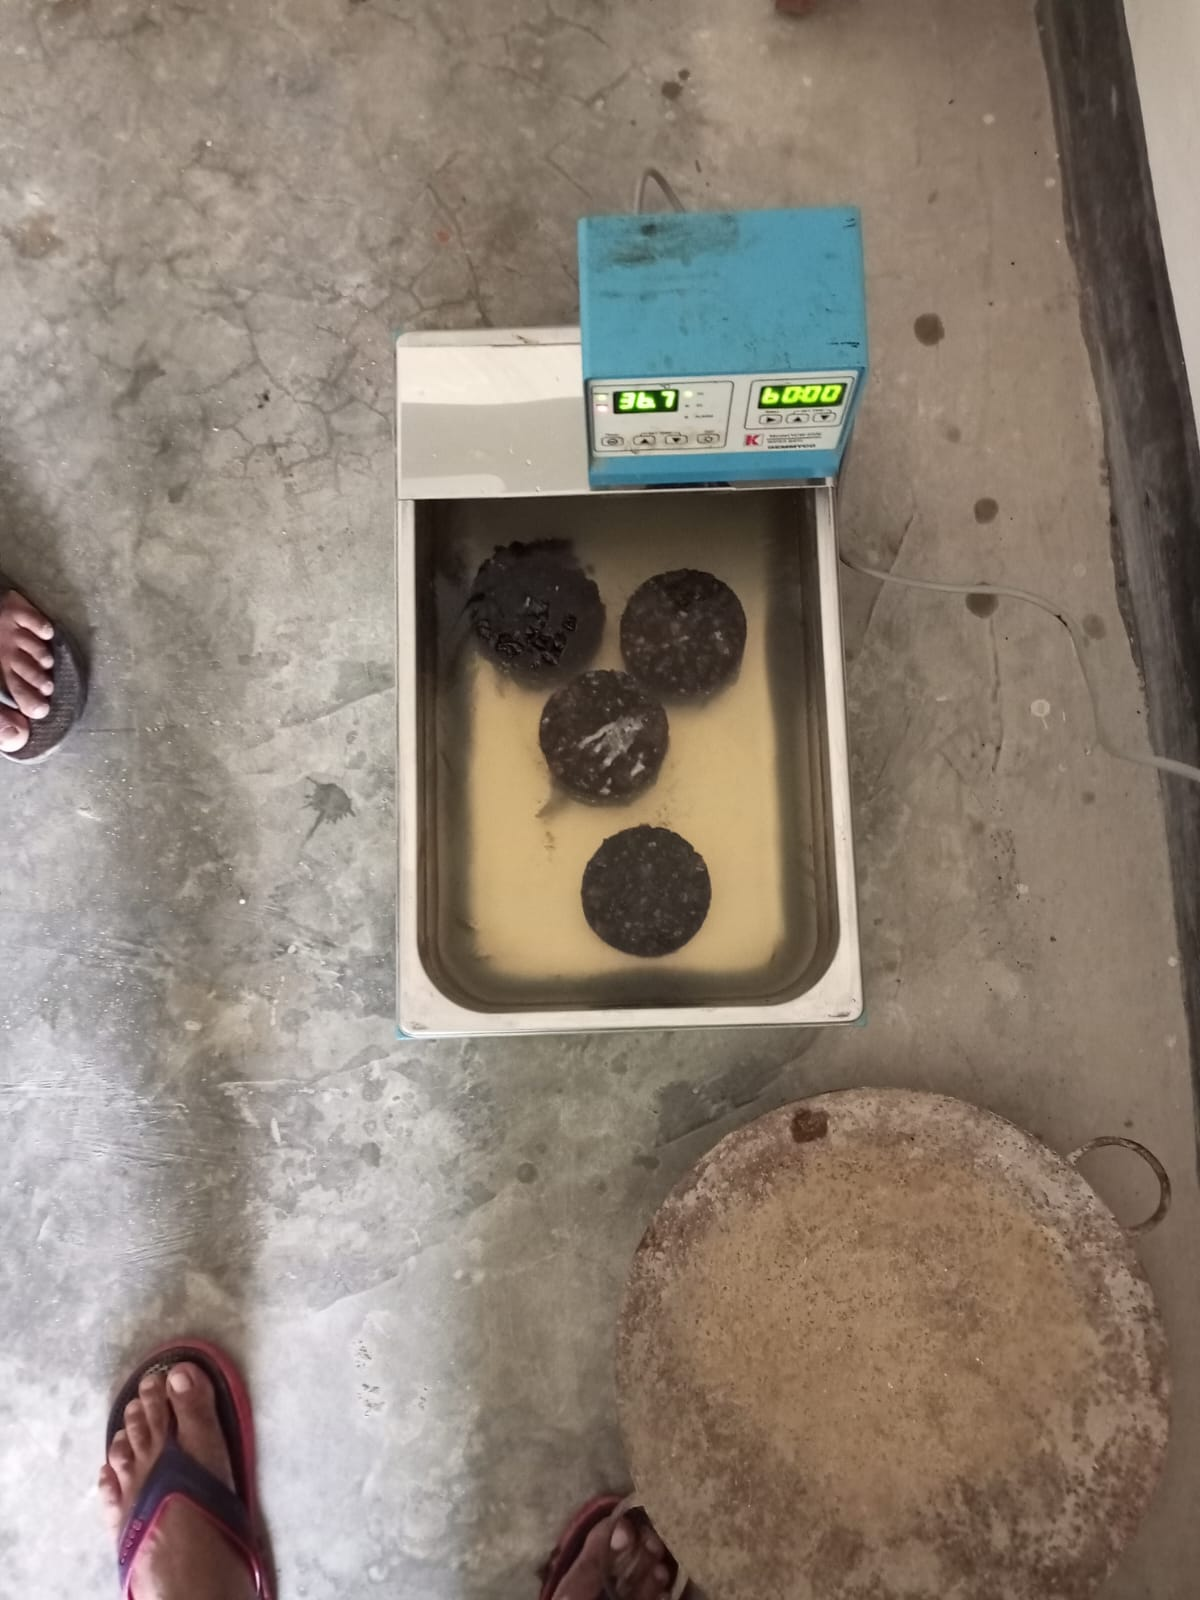
\includegraphics[width=4in, height=4in]{albums/appendix_34.jpeg}
\vspace{0.5cm}

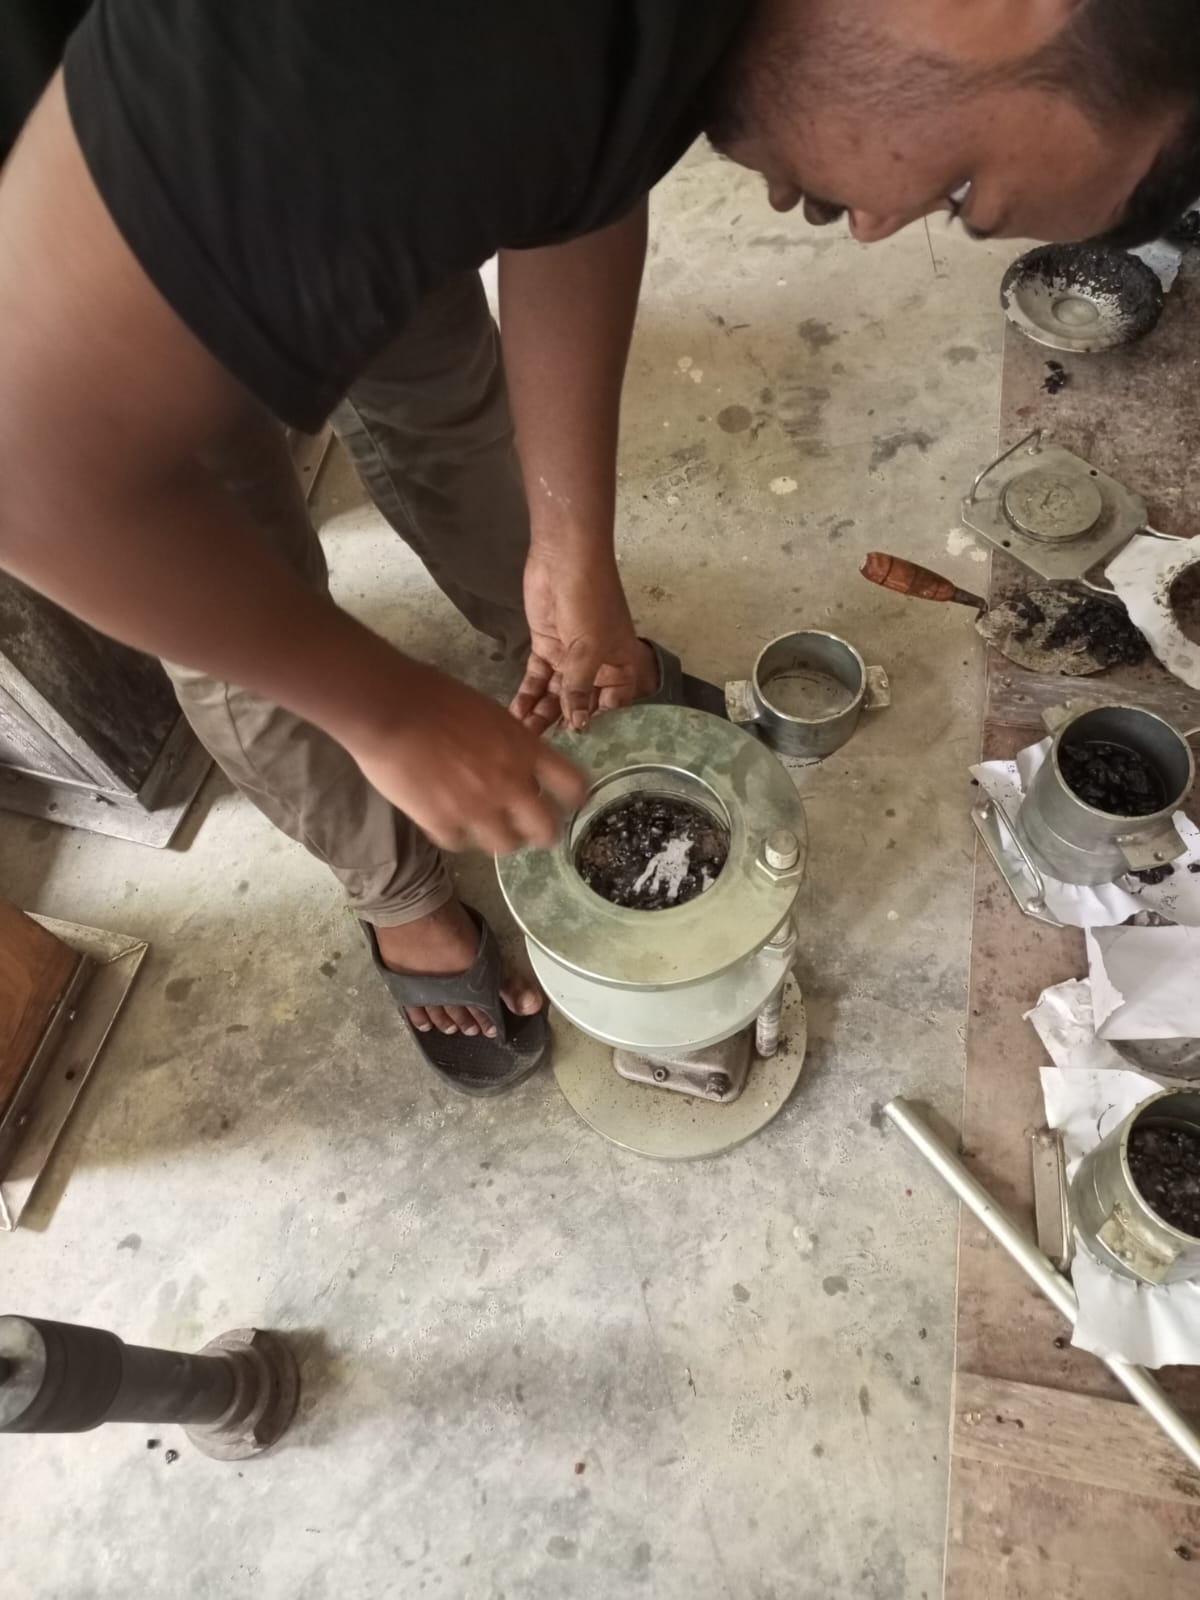
\includegraphics[width=4in, height=4in]{albums/appendix_35.jpeg}
\vspace{0.5cm}

\end{center}

\end{document}